%%%%%%%%%%%%%%%%%%%%%%%%%%%%%%%%%%%%%%%%%%%%%%%%%%%%%%%%%%%%%%%%%%%%%%
% Lớp 11 | Đường thẳng, mặt phẳng. Quan hệ song song trong | Điểm, đường thẳng và mặt phẳng
% Dạng 1H4?1-3: Tìm giao tuyến của hai mặt phẳng
% Số câu: 89  (sinh tự động bởi tach_cau.py; từ nay thầy sửa trực tiếp file này)
%%%%%%%%%%%%%%%%%%%%%%%%%%%%%%%%%%%%%%%%%%%%%%%%%%%%%%%%%%%%%%%%%%%%%%

%%%%%%%%%%%%%%%% TRẮC NGHIỆM 4 PHƯƠNG ÁN %%%%%%%%%%%%%%%%

% nguồn: Ok_Toan11_TracNghiem_Lan2
\begin{ex}%[1H4N1-3]%[ma:4eedc9b8]
	Cho tứ diện $ABCD$, $M$ là trung  điểm của $AB$, $N$ là điểm trên $AC$ mà $AN=\dfrac{1}{4}AC$, $P$ là điểm trên đoạn $AD$ mà $AP=\dfrac{2}{3}AD$. Gọi $E$ là giao điểm của $MP$ và $BD$, $F$ là giao điểm của $MN$ và $BC$. Khi đó giao tuyến của $\left( BCD \right)$ và $\left( CMP \right)$ là
	 \choice{$CP$}
		{$NE$} 
		 {$MF$}
		 {\True $CE$}
	 \loigiai{
		\begin{center}
			\begin{tikzpicture}[scale=1.7,font=\small,line join=round,line cap=round,>=stealth]
					 \path
						(0,0)  coordinate (B)
						($(B)+(1.5,-1)$) coordinate  (C)
						 ($(B)+(4,0)$) coordinate (E)
						($(B)!.5!(E)$)  coordinate (D)
						 ($(B)+(1,2)$) coordinate (A)
						($(A)!0.5!(B)$) coordinate (M) 
						($(A)!0.25!(C)$)  coordinate (N)
						(intersection of M--E and A--D) coordinate (P) 
						(intersection of M--N and  B--C) coordinate (F);
					\draw (A)--(B)--(C)--(E)--(P)--(A) 
						(B)--(F)--(N) 
						 (M)--(C)--(P)
						(A)--(C); 
					\draw [dashed] (M)--(P) 
						(B)--(E) 
						(P)--(D)--(C); 
					\foreach \x/\g in {A/90,B/200,C/-45,E/0,P/45,D/-45,F/120,M/130,N/130} 
					\fill (\x) circle  (1pt)
						($(\g:2mm)+(\x)$) node  {$\x$};
				\end{tikzpicture}
		\end{center}
		Ta có $C\in \left( BCD \right)\cap \left( CMP \right)$ $\left( 1  \right)$.
		Lại có $BD\cap MP=E\Rightarrow \heva{&E\in  BD\Rightarrow E\in(BCD)\\&E\in MP\Rightarrow E\in (CMP)}(2)$.\\
		 Từ $\left( 1 \right)$ và $\left( 2 \right)$ $\Rightarrow \left( BCD \right)\cap \left( CMP \right)=CE$.
	 }
\end{ex}

% nguồn: Ok_Toan11_TracNghiem_Lan2
\begin{ex}%[1H4N1-3]%[ma:2d621db8]
	Cho bốn điểm $A,B,C,D$ không đồng phẳng. Gọi $I,K$ lần lượt là trung điểm hai  đoạn thẳng $AD$ và $BC$. $IK$ là giao tuyến của cặp mặt phẳng nào sau đây ?
	 \choice{$\left( IBC \right)$ và $\left( KBD \right)$}
		{$\left( IBC \right)$  và $\left( KCD \right)$}
		{\True $\left( IBC \right)$ và $\left( KAD  \right)$}
		{$\left( ABI \right)$  và $\left( KAD \right)$}
	\loigiai{ 
		\begin{center}
			\begin{tikzpicture}[scale=1.7,font=\small,line join=round,line cap=round,>=stealth]
					 \path
						 (0,0) coordinate (A)
						($(A)+(1,-1.5)$) coordinate (B) 
						 ($(A)+(3,0)$) coordinate (C)
						($(A)+(1,2)$) coordinate (D) 
						($(A)!0.5!(D)$)  coordinate (I)
						($(B)!0.5!(C)$) coordinate (K); 
					 \draw (A)--(B)--(C)--(D)--(A)
						 (B)--(D)
						 (I)--(B)
						 (D)--(K);
					 \draw[dashed] (A)--(K)--(I)--(C)--(A);
					\foreach \x/\g in  {A/180,B/-90,C/0,D/90,K/-45,I/135}
					\fill (\x) circle  (1pt)
						($(\g:2mm)+(\x)$)  node {$\x$};
				\end{tikzpicture}
		\end{center}
		$\heva{&I\in AD\subset(KAD)\\&I\in(IBC)}\Rightarrow I$ là điểm chung thứ nhất của hai mặt phẳng $\left( IBC \right)$ và  $\left( KAD \right)$.\\
		$\heva{&K\in BC\subset(IBC)\\&K\in (KAD)}\Rightarrow K$ là điểm chung thứ hai của hai mặt phẳng $\left( IBC \right)$  và $\left( KAD \right)$.\\
		Vậy $\left( IBC \right)\cap  \left( KAD \right)=IK$.
	 }
\end{ex}

% nguồn: Ok_Toan11_TracNghiem_Lan2
\begin{ex}%[1H4N1-3]%[ma:b51cb6f0]
	Cho hình chóp $S.ABCD$ có đáy $ABCD$ là hình thang với đáy  lớn $AD$, $AD=2BC$. Gọi $O$ là giao điểm của $AC$ và $BD$. Tìm giao tuyến của hai mặt phẳng $\left( SAC \right)$ và $\left( SBD \right)$.
	 \choice{$SA$}
		{$AC$} 
		{\True $SO$} 
		 {$SD$}
	\loigiai{ 
		\begin{center}
			\begin{tikzpicture}[scale=1.4,font=\small,line join=round,line cap=round,>=stealth]
					 \path
						(0,0)  coordinate (A)
						($(A)+(0.5,-1.5)$)  coordinate (B)
						($(B)+(2,0)$) coordinate  (C)
						 ($(A)+(4,0)$) coordinate (D)
						($(A)+(2,2)$)  coordinate (S)
						(intersection of A--C and  B--D) coordinate (O);
					 \draw (A)--(B)--(C)--(D)--(S)--(A)
						 (B)--(S)--(C);
					 \draw [dashed] (B)--(D)--(A)--(C)
						 (S)--(O);
					\foreach  \x/\g in {A/180,B/180,C/0,D/0,S/90,O/-90}
					 \fill (\x) circle (1pt)
						($(\g:3mm)+(\x)$)  node {$\x$};
				\end{tikzpicture}
		\end{center}
		Ta có: $S\in \left( SAC \right)\cap \left( SBD \right)$ suy ra $\heva{&O\in AC\subset(SAC)\\&O\in BD\subset(SAC)}\Rightarrow O\in(SAC)\cap (SBD)$.\\ 
		Nên $SO=\left( SAC \right)\cap \left( SBD  \right)$.
	} 
\end{ex}

% nguồn: Ok_Toan11_TracNghiem_Lan2
\begin{ex}%[1H4N1-3]%[ma:57c1ec76]
	Cho  hình chóp $S.ABCD$ có đáy là hình thang $ABCD(AD//BC)$. Gọi $M$ là trung điểm của $CD$. Giao tuyến của hai mặt phẳng $\left( MSB \right)$ và $\left( SAC \right)$ là:
	\choice{$SP$  với $P$ là giao điểm của $AB$ và $CD$}
		{\True $SI$ với $I$ là giao điểm của $AC$  và $BM$}
		{$SO$ với $O$ là giao điểm của $AC$ và  $BD$}
		{$SJ$ với $J$ là giao điểm của  $AM$ và $BD$}
	\loigiai{ 
		\begin{center}
			\begin{tikzpicture}[scale=1.4,font=\small,line join=round,line cap=round,>=stealth]
					\path 
						(0,0) coordinate (A) 
						($(A)+(0.5,-1.5)$) coordinate  (B)
						($(B)+(2,0.3)$)  coordinate (C)
						($(A)+(4,0)$) coordinate  (D)
						($(A)+(2,2)$)  coordinate (S)
						($(C)!0.5!(D)$) coordinate  (M)
						(intersection  of A--C and B--M) coordinate (I);
					\draw (A)--(B)--(C)--(D)--(S)--(A) 
						(B)--(S)--(C) 
						 (S)--(M);
					\draw  [dashed] (D)--(A)--(C)
						 (B)--(M);
					\foreach \x/\g in  {A/180,B/180,C/0,D/0,S/90,I/90,M/0}
					\fill (\x)  circle (1pt)
						($(\g:3mm)+(\x)$) node {$\x$}; 
				\end{tikzpicture}
		\end{center}
		Giao tuyến của hai mặt phẳng $\left( MSB \right)$ và $\left(  SAC \right)$ là $SI$ với $I$ là giao điểm của $AC$ và $BM$.
	} 
\end{ex}

% nguồn: Ok_Toan11_TracNghiem_Lan2
\begin{ex}%[1H4N1-3]%[ma:70cb0c37]
	Cho hình chóp $S.ABCD$ với $ABCD$ là hình bình hành.  Khi đó giao tuyến của hai mặt phẳng $\left( SAC \right)$ và $\left( SAD \right)$ là
	\choice{Đường thẳng  $SC$}
		{Đường  thẳng $SB$}
		{Đường thẳng $SD$} 
		 {\True Đường thẳng $SA$}
	 \loigiai{
		Ta  thấy $\left( SAC \right)\cap \left( SAD \right)=SA$.
	} 
\end{ex}

% nguồn: Ok_Toan11_TracNghiem_Lan2
\begin{ex}%[1H4N1-3]%[ma:b5d59022]
	Cho hình chóp $S.ABCD$ có đáy là hình bình hành.  Gọi $M$, $N$ lần lượt là trung điểm của $AD$ và $BC$. Giao tuyến của $\left( SMN \right)$ và $\left( SAC \right)$ là
	 \choice{$SK$ ( $K$ là trung điểm của $AB$)}
		{\True  $SO$ ( $O$ là tâm của hình bình hành $ABCD$)}
		{$SF$ ( $F$  là trung điểm của $CD$)}
		{$SD$} 
	 \loigiai{
		\begin{center}
			\begin{tikzpicture}[scale=1.2,font=\small,line join=round,line cap=round,>=stealth]
					 \def\a{4}
					\path (0:0) coordinate  (A)
						 ++(0:\a) coordinate (D)
						++(-130:\a/2) coordinate  (C)
						($(A)+(C)-(D)$) coordinate (B) 
						 ($(A)+(80:\a)$) coordinate (S)
						 (intersection of A--C and B--D) coordinate (O)
						($(A)!.5!(D)$) coordinate  (M)
						($(B)!.5!(C)$) coordinate (N); 
					 \draw[dashed] (S)--(M)--(N)
						(A)--(C) 
						 (B)--(D)
						(B)--(A)--(D) 
						 (A)--(S);
					\draw (S)--(N) 
						 (B)-- (C)--(D)
						(B)--(S) 
						 (C)--(S)
						(D)--(S); 
					\foreach  \x/\g in {A/135,B/-135,C/-45,D/45,S/90,M/150,N/-90,O/-60}
					\fill  (\x) circle (1pt)
						 ($(\g:3mm)+(\x)$) node {$\x$};
				\end{tikzpicture}
		\end{center}
		Gọi $O$ là tâm hbh $ABCD$  $\Rightarrow O=AC\cap MN$ $\Rightarrow SO=\left( SMN \right)\cap \left( SAC \right)$.
	 }
\end{ex}

% nguồn: Ok_Toan11_TracNghiem_Lan2
\begin{ex}%[1H4N1-3]%[ma:d72041b1]
	Cho hình chóp tứ giác $S.ABCD$. Giao tuyến của  hai mặt phẳng $\left( SAB \right)$ và $\left( SBC \right)$ là
	\choice{$SA$} 
		{\True  $SB$}
		{$SC$} 
		{$AC$} 
	 \loigiai{
		Ta có: $\heva{&S\in(SAB)\cap (SBC)\\&B\in (SAB)\cap(SBC)}\Rightarrow  SB$ là giao tuyến của hai mặt phẳng $\left( SAB \right)$ và $\left( SBC \right)$.
	 }
\end{ex}

% nguồn: Ok_Toan11_TracNghiem_Lan2
\begin{ex}%[1H4N1-3]%[ma:68c7f5e3]
	Cho hình  chóp $S.ABCD$, biết $AC$ cắt $BD$ tại $M$, $AB$ cắt $CD$ tại $O$. Tìm giao tuyến của hai mặt phẳng $\left( SAB \right)$ và $\left( SCD \right)$.
	\choice{\True $SO$} 
		{$SM$} 
		 {$SA$}
		 {$SC$}
	\loigiai{ 
		\begin{center}
			\begin{tikzpicture}[scale=1.4,font=\small,line join=round,line cap=round,>=stealth]
					 \path
						(0,0) coordinate  (A)
						($(A)+(1,-1)$) coordinate  (B)
						 ($(B)+(2,-0.3)$) coordinate (C)
						($(A)+(4,0)$)  coordinate (D)
						($(A)+(2,2)$) coordinate  (S)
						(intersection  of A--C and B--D) coordinate (M)
						 (intersection of A--B and C--D) coordinate (O);
					\draw (A)--(B) 
						 (C)--(D)--(S)--(A)
						 (B)--(S)--(C)
						 (B)--(O)--(C)
						 (S)--(O);
					 \draw [dashed] (D)--(A)--(C)
						 (B)--(D)
						(B)--(C); 
					\foreach \x/\g in  {A/180,B/180,C/0,D/0,S/90,M/90,O/-90}
					\fill (\x) circle  (1pt)
						($(\g:3mm)+(\x)$) node {$\x$}; 
				\end{tikzpicture}
		\end{center}
		Ta  có: $\heva{&O=AB\cap CD\\&AC\subset (SAB)\\&CD\subset (SAC)}\Rightarrow O\in(SAB)\cap(SCD)$.
		Lại có: $S\in \left( SAB \right)\cap \left( SCD \right)$; $S\ne  O$.\\
		Khi đó $\left( SAB \right)\cap \left( SCD \right)=SO$. 
	 }
\end{ex}

% nguồn: Ok_Toan11_TracNghiem_Lan2
\begin{ex}%[1H4N1-3]%[ma:0639ba12]
	Cho tứ diện $ABCD$. Giao tuyến của hai mặt  phẳng $\left(ABC\right)$ và $\left(CDA\right)$ là đường thẳng
	\choice 
		{\True $AC$} 
		{$CD$} 
		{$AB$} 
		{$BD$} 
	 \loigiai{
	 \immini{
		 Ta có $\heva{
		& A\in\left(ABC\right)\cap\left(CDA\right)\\ 
		& C\in\left(ABC\right)\cap\left(CDA\right)}\Rightarrow\left(ABC\right)\cap\left(CDA\right)=AC$.} 
		{\begin{tikzpicture}[line join=round,line cap=round]
		\coordinate  (A) at (-1,4);
		\coordinate (B)  at (-2,0);
		 \coordinate (C) at (0,-3);
		 \coordinate (D) at (3,0);
		\draw  (A)--(B)
			 (A)--(C)
			(A)--(D) 
			(C)--(D) 
			(B)--(C); 
		\draw[dashed,thin](B)--(D); 
		\foreach  \i/\g in {A/90,B/180,C/-90,D/0}{\draw[fill=black](\i) circle (1pt)
			($(\i)+(\g:3mm)$) node[scale=1]{$\i$};} 
	\end{tikzpicture}
		 }
	 }
\end{ex}

% nguồn: Ok_Toan11_TracNghiem_Lan2
\begin{ex}%[1H4N1-3]%[ma:9dc310fd]
	Cho hình chóp $S.ABCD$ có đáy $ABCD$ là hình bình hành. Gọi $I$ và $J$ lần lượt là  trung điểm của $SA$ và $SB$. Khẳng định nào sau đây sai?
	\choice{$\left( SAB \right)\cap \left( IBC \right)=IB$} 
		 {$IJCD$ là hình thang}
		{$\left(  SBD \right)\cap \left( JCD \right)=JD$}
		{\True $\left( IAC \right)\cap  \left( JBD \right)=AO$ ( $O$ là tâm $ABCD$)}
	\loigiai{ 
		\begin{center}
			\begin{tikzpicture}[scale=1.2,font=\small,line join=round,line cap=round,>=stealth]
					 \path
						(0,0) coordinate  (D)
						($(D)+(-1,-2)$)  coordinate (A)
						($(A)+(4,0)$) coordinate (B) 
						($(D)+(4,0)$)  coordinate (C)
						 ($(D)+(0,3)$) coordinate (S)
						($(S)!0.5!(A)$) coordinate  (I)
						 ($(S)!0.5!(B)$) coordinate (J)
						($(A)!0.5!(C)$) coordinate  (O);
					 \draw (A)--(B)--(C)--(S)--(A)
						(S)--(B) 
						(C)--(J)--(I); 
					\draw  [dashed] (A)--(D)--(C)--(A)
						(S)--(D)--(B) 
						 (I)--(D)
						(C)--(I) 
						 (S)--(O)
						 (D)--(J);
					\foreach  \x/\g in {D/190,A/180,B/0,C/0,S/90,J/45,I/170,O/-90}
					\fill  (\x) circle (1pt)
						($(\g:3mm)+(\x)$)  node {$\x$};
				\end{tikzpicture}
		\end{center}
		Ta có: $\left( IAC \right)\cap \left( JBD \right)=\left( SAC \right)\cap \left( SBD \right)=SO$. 
	} 
\end{ex}

% nguồn: Ok_TracNghiemLop11_Lan1
\begin{ex}%[1H4N1-3]%[ma:c78f23fb]
	\immini[thm]{Cho hình chóp $S.ABCD$ có  đáy $ABCD$ là hình thang, đáy lớn $AD$.
	Khi đó giao tuyến của hai mặt phẳng $(SAB)$ và $(SCD)$ là}{	\begin{tikzpicture}[scale=.8]
		 \def\a{5}
		 \def\h{4}
		\path (0:0) coordinate  (A)
			++(0:\a) coordinate  (D)
			($(A)+(-130:\a/2)$) coordinate (B) 
			($(D)+(B)-(A)$)  coordinate (Ct)
			($(B)!1/2!(Ct)$)  coordinate (C)
			($(A)+(80:\h)$)  coordinate (S)
			(intersection of A--C and B--D) coordinate (O); 
		 \draw[dashed] (D)--(A)--(B)
			 (A)--(S);
		\draw (B)--(C)--(D) 
			(D)--(S) 
			 (C)--(S)
			 (B)--(S);
		\foreach \x/\g in  {A/135,D/45,C/-45,B/-135,S/90}
		\fill[black] (\x) circle  (1pt)
			($(\g:3mm)+(\x)$)  node {$\x$};
	\end{tikzpicture}
	} 
	 \choice
		{Đường thẳng $SO$ với $O$ là giao điểm của $AC$  và $BD$}
		{Đường thẳng đi qua $S$  và song song $AC$}
		{Đường thẳng đi qua $S$ và song  song $BD$}
		{\True Đường  thẳng $SI$ với $I$ là giao điểm của $AB$ và $CD$}
	\loigiai{ 
		Xét $(SAB)$ và  $(SCD)$ có
		\begin{itemize}
			\item $S\in(SAB)\cap(SCD)$. 
			\item Gọi $I=AB\cap CD\Rightarrow  I\in(SAB)\cap(SCD)$.
		\end{itemize}
		Suy ra  $(SAB)\cap(SCD)=SI$.
	 }
\end{ex}

% nguồn: Ok_TracNghiemLop11_Lan1
\begin{ex}%[1H4N1-3]%[ma:c1cffb7d]
	Cho tứ diện $ ABCD$ có $E$, $F$ lần lượt là trung điểm cạnh $BC$, $CD$ và $G$ là trọng tâm tam giác $ACD$. Giao tuyến của hai mặt phẳng $(ABG)$ và  $(ACD)$ là đường thẳng nào dưới đây?
	\choice 
		 {$AE$}
		 {\True $AF$}
		{$CD$} 
		 {$BG$}
	 \loigiai{
	\immini{ 
		Ta có $A$, là điểm  chung của hai mặt phẳng $(ABG)$ và $(ACD)$.\\
		Lại có $\heva{&F\in AG,~AG\in (ABG) \Rightarrow F \in (ABF)\\ &  F \in CD,~CD\in (ACD)\Rightarrow F \in (ACD).}$\\
		Suy ra,  $F$ cũng là điểm chung của hai mặt phẳng $(ABF)$ và $(ACD)$.\\
		Vậy $AF$  là giao tuyến của hai mặt phẳng $(ABF)$ và $(ACD)$.
		}{ 
		\begin{tikzpicture}[scale=0.8,font=\footnotesize,line join=round,line cap=round]
				\coordinate  (A) at (0,4);
				 \coordinate (B) at (-2.5,0);
				\coordinate  (C) at (1,-2.5);
				\coordinate (D)  at (3,0);
				\coordinate (E) at  ($(B)!0.5!(C)$);
				\coordinate (F)  at ($(C)!0.5!(D)$);
				\coordinate (G) at  ($(A)!0.667!(F)$);
				 \draw (A)--(B)--(C)--(D)--(A)--(C)
					 (A)--(F);
				 \draw[dashed] (B)--(D)
					(G)--(B)--(F); 
				\foreach \i/\g in {A/90,B/-180,C/-90,D/0,E/-90,F/-90,G/0}{\draw[fill](\i) circle  (1pt)
					 ($(\i)+(\g:3mm)$) node {$\i$};}
			\end{tikzpicture}
		} 
	} 
\end{ex}

% nguồn: Ok_TracNghiemLop11_Lan1
\begin{ex}%[1H4N1-3]%[ma:ca5ea3a5]
	Cho hình chóp $S.ABCD$ có đáy là hình thang $ABCD$ ($AB\parallel CD$). Khẳng định  nào sau đây \textbf{sai}?
	 \choice
		{Hình  chóp $S.ABCD$ có $4$ mặt bên}
		{Giao tuyến của hai mặt phẳng $(SAC)$ và $(SBD)$ là $SO$ ($O$ là giao điểm  của $AC$ và $BD$)}
		{Giao tuyến của hai mặt phẳng $(SAD)$ và $(SBC)$ là $SI$ ($I$  là giao điểm của $AD$ và $BC$)}
		 {\True Giao tuyến của hai mặt phẳng $(SAB)$ và $(SAD)$ là đường đi qua $S$ và song song với $AB$}
	\loigiai{ 
		\begin{center}
			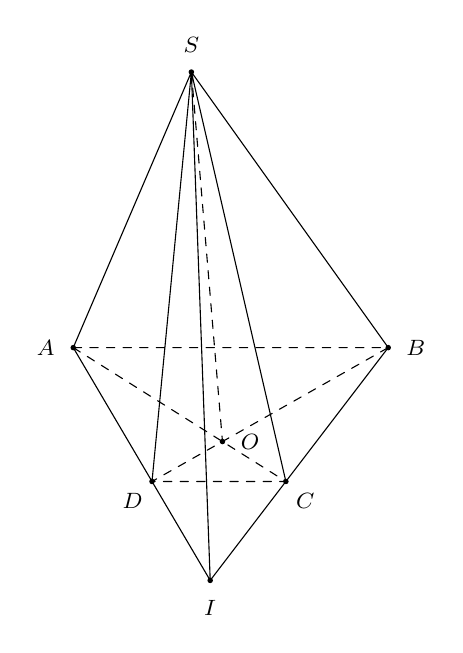
\begin{tikzpicture}[scale=1,font=\footnotesize,line join=round,line cap=round,>=stealth]
					 \coordinate (A) at (0,0);
					\coordinate (B)  at (4,0);
					\coordinate (C)  at (2.7,-1.7);
					\coordinate (D)  at (1,-1.7);
					\coordinate (S)  at (1.5,3.5);
					\coordinate (I)  at (intersection of A--D and B--C);
					\coordinate (O) at (intersection of A--C  and B--D);
					\draw[dashed] (A)--(B)--(D) 
						(A)--(C)--(D) 
						 (S)--(O);
					\draw (S)--(A)--(D)--(I)--(C)--(B)--(S)--(D) 
						 (I)--(S)--(C);
					\foreach \x/\g in{S/90,A/180,B/0,C/-45,D/-135,I/-90,O/0} \fill (\x) circle (1pt)+(\g:.35) node{$\x$}; 
				\end{tikzpicture}
		\end{center}
	Khẳng định \textbf{sai} là giao tuyến  của hai mặt phẳng $(SAB)$ và $(SAD)$ là đường đi qua $S$ và song song với $AB$ vì giao tuyến của hai mặt phẳng $(SAB)$ và $(SAD)$ phải là đường thẳng $SA$.}
\end{ex}

% nguồn: Ok_TracNghiemLop11_Lan1
\begin{ex}%[1H4N1-3]%[ma:8855c533]
	Cho hình chóp $S.ABCD$ với $ABCD$ là hình bình hành. Khi đó giao tuyến  của hai mặt phẳng $(SAC)$ và $(SAD)$ là
	 \choice
		{Đường  thẳng $SD$}
		{Đường  thẳng $SB$}
		{Đường thẳng $SC$} 
		{\True Đường thẳng $SA$} 
	\loigiai{ 
	\immini{Khi đó giao tuyến của hai mặt phẳng $(SAC)$ và $(SAD)$ là  $SA$.
		 }{
		\begin{tikzpicture}[scale=0.7]
				\def\a{4} 
				 \path (0:0) coordinate (A)
					++(0:\a)  coordinate (D)
					++(-130:\a/2)  coordinate (C)
					($(A)+(C)-(D)$) coordinate  (B)
					($(A)+(80:\a)$)  coordinate (S)
					(intersection of A--C and  B--D) coordinate (O);
				\draw[dashed]  (B)--(A)--(D)
					(A)--(S); 
				\draw (B)--  (C)--(D)
					(B)--(S) 
					(C)--(S) 
					 (D)--(S);
				\foreach \x/\g in  {A/135,B/-135,C/-45,D/45,S/90}
				\fill[black]  (\x) circle (1pt)
					($(\g:3mm)+(\x)$) node {$\x$}; 
			\end{tikzpicture}
		 }
	} 
\end{ex}

% nguồn: Ok_TracNghiemLop11_Lan1
\begin{ex}%[1H4N1-3]%[ma:4fac30a0]
	Cho tứ diện $ABCD$. Gọi $M$, $N$ lần lượt là trung điểm của $AC$ và  $DC$. Giao tuyến của hai mặt phẳng $(MBD)$ và $(ABN)$ là
	\choice 
		{Đường thẳng  $MN$}
		{Đường  thẳng $AM$}
		{\True  Đường thẳng $BG$ ($G$ là trọng tâm $\triangle ACD$)}
		{Đường thẳng $AH$ ($H$ là  trực tâm $\triangle ACD$)}
	 \loigiai{
	 \immini{
		Vì $G$ là  trọng tâm $\triangle ACD$ nên $G$ là giao điểm của hai trung tuyến $DM$ và $AN$ .\\
		Suy ra $G$ là điểm chung  của $(MBD)$ và $(ABN)$.\\
		Lại có  $B$ cũng là điểm chung của $(MBD)$ và $(ABN)$.\\
		 Vậy $BG$ là giao tuyến của hai mặt phẳng $(MBD)$ và $(ABN)$.
		}{	\begin{tikzpicture}[scale=0.8,font=\footnotesize,line join=round,line cap=round]
		 \coordinate (A) at (0,4);
		\coordinate  (B) at (-2.5,0);
		\coordinate (C) at  (1,-2.5);
		\coordinate (D) at (3,0); 
		\coordinate (M)  at ($(A)!0.5!(C)$);
		\coordinate (N) at ($(C)!0.5!(D)$); 
		\coordinate (G)  at ($(D)!0.667!(M)$);
		 \draw (A)--(B)--(C)--(D)--(A)--(C)
			 (B)--(M)--(D)
			 (A)--(N);
		\draw[dashed]  (B)--(D)
			 (B)--(N);
		\foreach \i/\g in {A/90,B/-180,C/-90,D/0,M/150,N/-70,G/50}{\draw[fill](\i)  circle (1pt)
			 ($(\i)+(\g:3mm)$) node {$\i$};}
	\end{tikzpicture}
	}} 
\end{ex}

% nguồn: Ok_TracNghiemLop11_Lan1
\begin{ex}%[1H4N1-3]%[ma:7ec20472]
	Cho hình chóp tứ giác $S.ABCD$ có đáy $ABCD$ là hình bình hành. Gọi $O$ là giao điểm  của $AC$ và $BD$. Trong các đường thẳng sau, đường thẳng nào là giao tuyến của hai mặt phẳng $\left(SAC\right)$ và $\left(SBD\right)$
	\choice 
		 {$SA$}
		{$AC$} 
		 {\True $SO$}
		 {$SD$}
	 \loigiai{
	\immini{ 
		Vì $S$, $O$ cùng thuộc hai mặt phẳng $(SAC)$ và $(SBD)$  nên giao tuyến của mặt phẳng $(SAC)$ với mặt phẳng $(SBD)$ là đường thẳng $SO$.}
		{\begin{tikzpicture}[scale=.7]
		\def\a{4} 
		 \path (0:0) coordinate (A)
			++(0:\a)  coordinate (D)
			++(-50:.55*\a)  coordinate (C)
			($(A)+(C)-(D)$)  coordinate (B)
			(intersection of A--C and B--D) coordinate (O) 
			 ($(O)+(70:\a)$) coordinate (S);
		\draw[dashed] (A)--(D)--(C) 
			 (D)--(S)
			(S)--(O) 
			(A)--(C) 
			 (B)--(D);
		\draw (A)-- (B)--(C) 
			 (B)--(S)
			 (C)--(S)
			(A)--(S); 
		\foreach \x/\g  in {A/180,B/-135,C/-45,D/0,S/90,O/-90}
		\fill[black]  (\x) circle (1pt)
			($(\g:3mm)+(\x)$) node  {$\x$};
	\end{tikzpicture}
		} 
	 }
\end{ex}

% nguồn: Ok_Toan11_TracNghiem_Lan2
\begin{ex}%[1H4H1-3]%[ma:7a3d8f12]
	Cho hình chóp $S.ABCD$ có đáy là hình bình hành tâm $O$. Gọi $M$, $N$  lần lượt là trung điểm $AD$ và $BC$ Giao tuyến của hai mặt phẳng $(SMN)$ và $(SAC)$ là
	\choice 
		 {$SM$}
		 {$SN$}
		 {\True $SO$}
		{$SA$} 
	\loigiai{ 
		\begin{center}
			\begin{tikzpicture}[scale=1,font=\footnotesize,line join=round,line cap=round,>=stealth]
					 \def\bc{3.5}
					\def\ba{2} 
					 \def\h{4}
					\def\gocB{25} 
					\coordinate[label=below  left:$B$] (B) at (0,0);
					\coordinate[label=above  right:$A$] (A) at (\gocB:\ba);
					\coordinate[label=below:$C$] (C)  at (\bc,0);
					\coordinate[label=right:$D$] (D) at  ($(C)-(B)+(A)$);
					\coordinate[label=below:$N$] (N)  at ($(B)!1/2!(C)$);
					\coordinate[label=above:$M$] (M)  at ($(A)!1/2!(D)$);
					\coordinate[label=below:$O$] (O) at  ($(A)!1/2!(C)$);
					\coordinate[label=above left:$S$] (S)  at ($(B)+(70:\h)$);
					\draw  (B)--(C)--(D)--(S)--cycle (N)-- (S)--(C);
					\draw[dashed] (A)--(D) 
						 (S)--(A)--(B)
						 (A)--(C)
						 (M)--(N)
						 (O)--(S)--(M);
					\foreach \diem in {A,B,C,D,S,M,N,O} \fill (\diem) circle (1pt); 
				\end{tikzpicture}
		\end{center}
		Có $S$ là điểm chung thứ nhất của  hai mặt phẳng $(SMN)$ và $(SAC) $\\
		Từ  giả thiết, suy ra $O\in MN.$\\
		Do đó $\heva{& O\in AC\subset (SAC) \\  & O\in MN\subset (SMN)}\Rightarrow O$ là điểm chung thứ hai của hai mặt phẳng $(SMN)$ và\\
		 $(SAC) $\\
	Vậy $(SMN)\cap  (SAC)=SO.$}
\end{ex}

% nguồn: Ok_Toan11_TracNghiem_Lan2
\begin{ex}%[1H4H1-3]%[ma:be825dd7]
	Cho hình chóp $S.ABCD$, đáy $ABCD$ là hình thang có $2$ đáy là $AD$ và  $BC$ Gọi $M$, $N$ lần lượt là trung điểm của $SB$, $SC$, $O$ là giao điểm của $AC$ và $BD$. Giao tuyến của hai mặt $(AMN)$ và $(SBD)$ là
	 \choice
		{$DN$} 
		{\True $DM$} 
		 {$OM$}
		 {$SO$}
	\loigiai{ 
		\begin{center}
			\begin{tikzpicture}[scale=1,font=\footnotesize,line join=round,line cap=round,>=stealth]
					\def\ad{4} 
					\def\ab{2} 
					\def\bc{2} 
					 \def\as{3.5}
					 \def\gocA{50}
					\def\gocB{130} 
					\coordinate[label=left:$A$] (A) at  (0,0);
					\coordinate[label=below  left:$B$] (B) at (-\gocA:\ab);
					\coordinate[label=below right:$C$] (C) at  ($(B)+(180-\gocA-\gocB:\bc)$);
					\coordinate[label=right:$D$] (D)  at (\ad,0);
					\coordinate[label=above:$S$] (S)  at (65:\as);
					\coordinate[label=above  left:$M$] (M) at ($(S)!0.5!(B)$);
					\coordinate[label=right:$N$] (N) at  ($(S)!0.5!(C)$);
					\coordinate[label=below:$O$] (O) at (intersection of A--C and  B--D);
					 \draw (A)--(B)--(C)--(D)--(S)--cycle (B)--(S)--(C)
						 (M)--(N);
					\draw[dashed]  (C)--(A)--(D)
						(B)--(D) 
						(N)--(A)--(M); 
					\foreach \diem in {A,B,C,D,S,M,O,N} \fill  (\diem) circle (1pt);
				\end{tikzpicture}
		\end{center}
		Ta có $MN$ là đường trung bình của tam giác  $SBC$, suy ra $MN\parallel BC$\\
		Ta lại có  $BC\parallel AD$, suy ra $MN\parallel AD$\\
	Khi đó $(AMN)\equiv (AMND)\Rightarrow (AMN)\cap (SBD)=MD$.} 
\end{ex}

% nguồn: Ok_Toan11_TracNghiem_Lan2
\begin{ex}%[1H4H1-3]%[ma:43c09b1f]
	Cho  hình chóp $S.ABCD$ có đáy là hình thang$ABCD(AD\parallel BC)$. Gọi $M$ là trung điểm của $CD$. Giao tuyến của hai mặt phẳng $(MSB)$ và $(SAC)$ là:
	\choice 
		{ $SP$  với $P$ là giao điểm của $AB$ và $CD$}
		{\True $SI$ với $I$ là giao điểm của  $AC$ và $BM$}
		{ $SO$ với $O$ là giao điểm  của $AC$ và $BD$}
		{ $SJ$ với  $J$ là giao điểm của $AM$ và $BD$}
	\loigiai{ 
		\begin{center}
			\begin{tikzpicture}[scale=1,font=\footnotesize,line join=round,line cap=round,>=stealth]
					 \def\ad{5}
					 \def\ab{2.5}
					\def\bc{2.5} 
					\def\as{3.5} 
					\def\gocA{50} 
					 \def\gocB{120}
					\coordinate[label=left:$A$] (A)  at (0,0);
					\coordinate[label=below left:$B$] (B) at (-\gocA:\ab); 
					 \coordinate[label=below right:$C$] (C) at ($(B)+(0:\bc)$);
					\coordinate[label=right:$D$]  (D) at (\ad,0);
					\coordinate[label=above:$S$]  (S) at (90:\as);
					\coordinate[label=right:$M$] (M) at ($(C)!0.5!(D)$); 
					\coordinate[label=below:$I$] (I) at (intersection of A--C  and B--M);
					 \draw (A)--(B)--(C)--(D)--(S)--cycle (B)--(S)--(C)
						 (S)--(M);
					\draw[dashed]  (D)--(A)--(C)
						(M)--(B); 
					\foreach \diem in {A,B,C,D,S,M,I} \fill (\diem) circle (1pt); 
				\end{tikzpicture}
		\end{center}
	Giao tuyến của hai mặt phẳng $(MSB)$ và $(SAC)$ là $SI$ với $I$ là giao điểm  của $AC$ và $BM$.}
\end{ex}

% nguồn: Ok_Toan11_TracNghiem_Lan2
\begin{ex}%[1H4H1-3]%[ma:44e4917e]
	Cho hình chóp tứ giác $S.ABCD$ có đáy là hình thang  $\left(AD//BC\right)$ . Gọi $H$ là trung điểm $AB$ . Giao tuyến của hai mặt phẳng $\left(SHD\right)$ và $\left(SAC\right)$ là:
	\choice 
		 {\True $SI$ ($I$ là giao điểm của $HD$ và $AC$)}
		{$SK$ ($K$  là giao điểm của $AB$ và $CD$)}
		{$SO$ ($O$  là giao điểm của $AC$ và $BD$)}
		 {$SA$}
	 \loigiai{
	\immini{ 
		$S$ là điểm chung thứ nhất của $\left(SHD\right)$  và $\left(SAC\right)$.\\
		Gọi $I$ là giao điểm của $AC$ và $HD$ nên $I\in AC$, $I\in HD$ do đó $I$  là điểm chung thứ hai $\left(SHD\right)$ và $\left(SAC\right)$.\\
		Vậy giao tuyến của hai mặt phẳng $\left(SHD\right)$ và  $\left(SAC\right)$ là $SI$.}
		{\begin{tikzpicture}[line join=round,line cap=round,scale=.7]
		\coordinate (S) at  (1,4);
		 \coordinate (A) at (-1,0);
		\coordinate  (B) at (1,-2);
		 \coordinate (C) at (3,-2);
		\coordinate (D)  at (6,0);
		\coordinate (H) at  ($(A)!0.5!(B)$);
		\coordinate (I) at (intersection of A--C and H--D); 
		\draw  (S)--(A)
			 (S)--(B)
			 (S)--(C)
			(S)--(D) 
			(B)--(C) 
			 (A)--(B)--(C)--(D)
			(S)--(H); 
		 \draw[dashed,thin](A)--(D)
			(A)--(C) 
			 (H)--(D);
		 \foreach \i/\g in {S/90,A/180,B/-90,C/-90,D/0,H/-150,I/-90}{\draw[fill=black](\i) circle (1pt)
			($(\i)+(\g:3mm)$)  node[scale=1]{$\i$};}
	\end{tikzpicture}
		} 
	 }
\end{ex}

% nguồn: Ok_Toan11_TracNghiem_Lan2
\begin{ex}%[1H4H1-3]%[ma:989eee64]
	Cho hình chóp  $S.ABCD$ có $AC\cap BD=M$ và $AD\cap BC=N$. Giao tuyến của mặt phẳng $(SAC)$ và mặt phẳng $(SBD)$ là đường thẳng
	\choice 
		 {\True $SM$}
		{  $SN$}
		{ $SC$} 
		{ $SB$} 
	 \loigiai{
		\begin{center}
			\begin{tikzpicture}[scale=1,font=\footnotesize,line join=round,line cap=round,>=stealth]
					 \def\ad{4}
					 \def\ab{2.5}
					\def\bc{2.5} 
					 \def\as{3.5}
					 \def\gocA{50}
					 \def\gocB{110}
					\coordinate[label=above left:$A$]  (A) at (0,0);
					 \coordinate[label=below left:$B$] (B) at (-\gocA:\ab);
					 \coordinate[label=below right:$C$] (C) at ($(B)+(180-\gocA-\gocB:\bc)$);
					\coordinate[label=above right:$D$] (D) at  (\ad,0);
					\coordinate[label=above:$S$] (S) at  (65:\as);
					\coordinate[label=right:$N$] (I) at (intersection of A--D and B--C); 
					\coordinate[label=below:$M$]  (O) at (intersection of A--C and B--D);
					\draw  (S)--(A)--(B)--(I)--(D)--(S)
						(B)--(S)--(C)--(D); 
					\draw[dashed]  (A)--(C)
						(B)--(D) 
						(S)--(O) 
						(A)--(D); 
					\foreach  \diem in {A,B,C,D,S,O,I} \fill (\diem) circle (1pt);
				\end{tikzpicture}
		\end{center}
	Giao tuyến của mặt phẳng $(SAC)$ và mặt phẳng  $(SBD)$ là đường thẳng $SM$.}
\end{ex}

% nguồn: Ok_Toan11_TracNghiem_Lan2
\begin{ex}%[1H4H1-3]%[ma:87126799]
	Cho tứ diện$ABCD$, $M$ là  trung điểm của $AB$, $N$ là điểm trên $AC$ mà $AN=\dfrac14AC$, $P$ là điểm trên đoạn $AD$ mà $AP=\dfrac23AD$. Gọi $E$ là giao điểm của $MP$ và $BD$, $F$ là giao điểm của $MN$ và $BC$. Khi đó giao tuyến của $(BCD)$ và $(CMP)$ là
	 \choice
		 {$CP$}
		 {$NE$}
		 {$MF$}
		 {\True $CE$}
	 \loigiai{
		\begin{center}
			\begin{tikzpicture}[scale=1,font=\footnotesize,line join=round,line cap=round,>=stealth]
					 \path
						 (0,0) coordinate (B)
						(3,-2)  coordinate (C)
						 (4,0) coordinate (D)
						(1.2,3.4)  coordinate (A)
						($(A)!0.5!(B)$) coordinate  (M)
						($(A)!1/4!(C)$) coordinate (N) 
						($(A)!2/3!(D)$)  coordinate (P)
						(intersection of M--P and  B--D) coordinate (E)
						(intersection of M--N and  B--C) coordinate (F);
					\draw (P)--(A)--(B)--(C)--cycle  (A)--(C)--(M)
						 (B)--(F)--(N)
						 (C)--(P)--(E)--(C);
					\draw[dashed] (B)--(D)--(C) 
						 (M)--(P)--(D)--(E);
					\foreach \p/\q  in {A/90,B/180,C/-90,D/40,M/140,N/30,P/30,E/0,F/180}
					\fill (\p)  circle (1.0pt)
						($(\p)+(\q:2.5mm)$) node{$\p$}; 
				\end{tikzpicture}
		\end{center}
		Ta có  $C\in(BCD)\cap(CMP)$.\hfill(1)\\
		Lại có $BD\cap MP=E\Rightarrow\heva{&E\in BD\Rightarrow E\in(BCD)\\&E\in MP\Rightarrow E\in(CMP)}.$\hfill(2)\\ 
	Từ  $(1)$ và $(2)\Rightarrow(BCD)\cap(CMP)=CE$.}
\end{ex}

% nguồn: Ok_Toan11_TracNghiem_Lan2
\begin{ex}%[1H4H1-3]%[ma:96413b4c]
	Cho hình chóp $S.ABCD$ có đáy $ABCD$ là hình thang với đáy lớn $AD$. Gọi $M$ là trung điểm của $CD$; $I$ là giao điểm của $AC$ và $BM$; $O$ là giao điểm của $AC$ và $BD$. Giao tuyến của hai mặt phẳng $(SAC)$ và $(SBM)$ là 
	\choice 
		{Đường thẳng  $AM$}
		{Đường thẳng  $SO$}
		{Đường thẳng $SI$} 
		 {Đường thẳng $SM$}
	 \loigiai{
		\begin{center}
			\begin{tikzpicture}[scale=1,font=\footnotesize,line join=round,line cap=round,>=stealth]
					 \def\ad{4}
					 \def\ab{2.5}
					 \def\bc{2.5}
					\def\as{3.5} 
					\def\gocA{60} 
					 \def\gocB{120}
					\coordinate[label=left:$A$] (A) at  (0,0);
					\coordinate[label=below  left:$B$] (B) at (-\gocA:\ab);
					\coordinate[label=below right:$C$]  (C) at ($(B)+(0:\bc)$);
					\coordinate[label=right:$D$] (D) at  (\ad,0);
					\coordinate[label=above:$S$] (S) at (60:\as); 
					 \coordinate[label=right:$M$] (M) at ($(C)!0.5!(D)$);
					\coordinate[label=above:$O$]  (O) at (intersection of A--C and B--D);
					\coordinate[label=below:$I$] (I) at (intersection of A--C  and B--M);
					\draw (A)--(B)--(C)--(D)--(S)--cycle (B)--(S)--(C) 
						 (S)--(M);
					\draw[dashed] (D)--(A)--(C) 
						 (B)--(D)
						 (S)--(I)
						 (M)--(B);
					\foreach \diem in  {A,B,C,D,S,O,M,I} \fill (\diem) circle (1pt);
				\end{tikzpicture}
		\end{center}
		Ta có:  $AC\cap BM=I$\\
		$S\in (SAC)\cap (SBM)$\\ 
		$\heva{& I\in \text{A}C\subset (SAC) \\ & I\in BM\subset (SBM)}\Rightarrow I\in  (SAC)\cap (SBM)$\\
	Vậy $SI=(SAC)\cap  (SBM)$}
\end{ex}

% nguồn: Ok_Toan11_TracNghiem_Lan2
\begin{ex}%[1H4H1-3]%[ma:68ea8d1e]
	Cho hình chóp $S.ABCD$ có $AD\cap BC=M$, $AB\cap CD=N$. Giao tuyến của hai mặt phẳng $(SAB)$ và  $(SCD)$ là
	\choice 
		 {$SM$}
		 {$SA$}
		 {$MN$}
		{\True  $SN$}
	 \loigiai{
		\begin{center}
			\begin{tikzpicture}[font=\footnotesize,line join=round,line cap=round,>=stealth,scale=1]
					\foreach \x/\y/\pos in {0/0/A,1/-1.5/B,3.2/-1/C,4/0/D,1.8/3.5/S} \path  ($(\x,\y)$) coordinate (\pos);
					\coordinate (N) at (intersection of A--B and C--D); 
					\coordinate (M) at  (intersection of A--D and C--B);
					\draw[dashed]  (A)--(D)
						 (B)--(C);
					 \draw (B)--(S)--(C)--(N)--(D)--(S)--(A)--(M)--(D)
						(S)--(M) 
						 (S)--(N)--(A);
					\foreach \x/\pos in {A/180,B/-150,C/-60,D/60,S/90,M/-90,N/0} \fill  (\x) circle (1pt) node[{shift=(\pos:0.25)}]{$\x$};
				\end{tikzpicture}
		\end{center}
		$S$ là điểm chung thứ nhất của hai mặt phẳng $(SAB)$  và $(SCD)$.\\
		Vì $AB\cap  CD=N$ nên $\heva{
		&N\in AB\subset(SAB)\\ 
		&N\in  CD\subset(SCD)\\}$.
		Do đó $N$ là điểm chung thứ hai  của hai mặt phẳng trên.\\
	Vậy $SN$ là giao  tuyến của hai mặt phẳng $(SAB)$ và $(SCD)$.}
\end{ex}

% nguồn: Ok_Toan11_TracNghiem_Lan2
\begin{ex}%[1H4H1-3]%[ma:c86dd2bd]
	Cho hình chóp $S.ABCD$ có đáy $ABCD$ là hình bình hành. Gọi $I$ và $J$ lần lượt là trung điểm của $SA$ và $SB$. Khẳng định nào sau đây  \textbf{sai}?
	 \choice
		 {$(SAB)\cap(IBC)=IB$}
		{$IJCD$ là  hình thang}
		 {$(SBD)\cap(JCD)=JD$}
		{\True $(IAC)\cap(JBD)=AO$ ($O$ là tâm  $ABCD$)}
	 \loigiai{
	\immini{Ta có  $(IAC)\cap(JBD)=(SAC)\cap(SBD)=SO$.
		}{\begin{tikzpicture}[scale=0.7,font=\footnotesize,line join=round,line cap=round,>=stealth]
		\def\bc{4} 
		\def\ba{2} 
		 \def\h{4}
		\def\gocB{30} 
		\coordinate[label=below  left:$B$] (B) at (0,0);
		\coordinate[label=above left:$A$] (A) at  (\gocB:\ba);
		\coordinate[label=below right:$C$] (C) at (\bc,0); 
		 \coordinate[label=right:$D$] (D) at ($(C)-(B)+(A)$);
		\coordinate[label=above:$S$] (S)  at ($(A)+(90:\h)$);
		\coordinate[label=above  right:$I$] (I) at ($(S)!0.5!(A)$);
		\coordinate[label=above right:$J$]  (J) at ($(S)!0.5!(B)$);
		\coordinate[label=below:$O$]  (O) at ($(A)!1/2!(C)$);
		 \draw (B)--(C)--(D)--(S)--cycle (S)--(C);
		\draw[dashed]  (A)--(D)
			(S)--(A)--(B) 
			 (A)--(C)--(I)
			(B)--(D)--(J) 
			(S)--(O); 
		\foreach  \diem in {A,B,C,D,S,I,J}\fill (\diem) circle (1pt);
	\end{tikzpicture}
		 }
	} 
\end{ex}

% nguồn: Ok_Toan11_TracNghiem_Lan2
\begin{ex}%[1H4H1-3]%[ma:5f3702ce]
	Cho hình chóp $S.ABCD$ có đáy $ABCD$ là hình thang với đáy lớn $AD$, $AD=2BC$. Gọi $O$ là giao điểm của $AC$ và $BD$ Tìm giao tuyến của  hai mặt phẳng $(SAC)$ và $(SBD)$
	 \choice
		 {$SA$}
		 {$AC$}
		 {\True $SO$}
		{$SD$} 
	 \loigiai{
		\begin{center}
			\begin{tikzpicture}[scale=1,font=\footnotesize,line join=round,line cap=round,>=stealth]
					 \def\ad{4}
					\def\ab{2.5} 
					 \def\bc{2.5}
					 \def\as{3.5}
					 \def\gocA{60}
					\def\gocB{120} 
					\coordinate[label=left:$A$] (A) at  (0,0);
					 \coordinate[label=below left:$B$] (B) at (-\gocA:\ab);
					 \coordinate[label=below right:$C$] (C) at ($(B)+(0:\bc)$);
					\coordinate[label=right:$D$] (D) at  (\ad,0);
					\coordinate[label=above:$S$]  (S) at (60:\as);
					\coordinate[label=below:$O$] (O) at (intersection of A--C and  B--D);
					 \draw (A)--(B)--(C)--(D)--(S)--cycle (B)--(S)--(C);
					\draw[dashed] (D)--(A)--(C) 
						(B)--(D) 
						 (S)--(O);
					\foreach \diem  in {A,B,C,D,S,O} \fill (\diem) circle (1pt);
				\end{tikzpicture}
		\end{center}
		Có  $S\in (SAC)\cap (SBD)$.\\
		$\heva{& O\in AC,AC\subset (SAC)  \\ & O\in BD,BD\subset (SAC)}\Rightarrow O\in (SAC)\cap (SBD)$.\\
	Nên $SO=(SAC)\cap (SBD)$.} 
\end{ex}

% nguồn: Ok_Toan11_TracNghiem_Lan2
\begin{ex}%[1H4H1-3]%[ma:69fe868d]
	Cho hình chóp $S.ABCD$ có $AC$ cắt $BD$ tại $M$ và $AB$ cắt $CD$ tại $N$. Giao tuyến của mặt phẳng $\left(SAC\right)$ và mặt phẳng $\left(SBD\right)$ là đường thẳng 
	 \choice
		 {$SB$}
		 {$SN$}
		{\True  $SM$}
		{$SC$} 
	 \loigiai{
	\immini{ 
		Hai mặt phẳng $\left(SAC\right)$ và $\left(SBD\right)$ có điểm chung $S$ và $M$ nên $\left(SAC\right)\cap\left(SBD\right)=SM$.}{\begin{tikzpicture}[line join=round,line cap=round]
		\coordinate  (S) at (1,4);
		\coordinate (A) at (0,0); 
		 \coordinate (D) at (1,-2);
		\coordinate (C) at (3,-3); 
		\coordinate  (B) at (5,0);
		\coordinate (M) at (intersection  of A--C and B--D);
		\coordinate (N)  at (intersection of A--B and C--D);
		\draw  (S)--(A)
			 (S)--(B)
			(S)--(C) 
			 (S)--(D)
			 (B)--(C)
			(A)--(D)--(C)--(B) 
			 (A)--(N)--(D);
		 \draw[dashed,thin](A)--(B)
			(A)--(C) 
			(B)--(D) 
			(S)--(M); 
		\foreach \i/\g  in {S/90,A/-135,D/-90,C/-90,B/0,M/-90,N/-180}{\draw[fill=black](\i) circle (1pt)
			($(\i)+(\g:3mm)$) node[scale=.8]{$\i$};} 
	\end{tikzpicture}
		 }
	} 
\end{ex}

% nguồn: Ok_Toan11_TracNghiem_Lan2
\begin{ex}%[1H4H1-3]%[ma:026d1f7f]
	Cho hình chóp $S.ABCD$ với đáy là tứ  giác $ABCD$ có các cặp cạnh đối không song song. Giả sử $AC\cap BD=O$ và $AD\cap BC=I$. Giao tuyến của hai mặt phẳng $(SAC)$ và $(SBD)$ là
	\choice 
		{\True $SO$} 
		{$SI$} 
		{$SC$} 
		 {$SB$}
	 \loigiai{
		\begin{center}
			\begin{tikzpicture}[scale=1,font=\footnotesize,line join=round,line cap=round,>=stealth]
					\def\ad{4} 
					\def\ab{1.5} 
					 \def\bc{2.5}
					\def\as{3.5} 
					 \def\gocA{50}
					\def\gocB{150} 
					 \coordinate[label=above left:$A$] (A) at (0,0);
					\coordinate[label=below left:$B$]  (B) at (-\gocA:\ab);
					\coordinate[label=below right:$C$] (C)  at ($(B)+(180-\gocA-\gocB:\bc)$);
					\coordinate[label=right:$D$] (D) at (\ad,0); 
					\coordinate[label=above:$S$] (S) at (65:\as); 
					\coordinate[label=below:$I$] (I) at (intersection  of A--D and B--C);
					 \coordinate[label=below:$O$] (O) at (intersection of A--C and B--D);
					\draw (B)--(C)--(D)--(S)--cycle  (B)--(S)--(C)
						(S)--(I)--(B); 
					 \draw[dashed] (C)--(A)--(D)
						(B)--(D) 
						(S)--(O) 
						 (S)--(A)--(B)
						(A)--(I); 
					\foreach \diem  in {A,B,C,D,S,O,I} \fill (\diem) circle (1pt);
				\end{tikzpicture}
		\end{center}
		Hai mặt phẳng $(SAC)$ và $(SBD)$ có $S$  là điểm chung thứ nhất.\\
		$\heva{ 
		&  O\in AC\subset (SAC) \\ & O\in BD\subset (SBD)} \Rightarrow O$ là điểm chung thứ hai.\\
		Vậy giao tuyến của  hai mặt phẳng $(SAC)$ và $(SBD)$ là $SO$.
	} 
\end{ex}

% nguồn: Ok_Toan11_TracNghiem_Lan2
\begin{ex}%[1H4H1-3]%[ma:9231126e]
	Cho bốn điểm $A$, $B$, $C$, $D$ không đồng phẳng. Gọi $I$, $K$ lần lượt là trung điểm hai đoạn thẳng $AD$ và $BC$. $IK$ là  giao tuyến của cặp mặt phẳng nào sau đây?
	 \choice
		 {$(IBC)$ và $(KBD)$}
		 {$(IBC)$ và $(KCD)$}
		{\True $(IBC)$ và  $(KAD)$}
		{$(ABI)$ và $(KAD)$} 
	\loigiai{ 
	 \immini{Ta có $I\in(IBC)$,
		$I\in AD, AD\subset (KAD)$ nên $I\in (KAD)$.\\  Do đó $I\in (IBC)\cap (KAD)$.\\
		 $K\in(KAD)$,
		$K\in BC, BC\subset (IBC)$ nên $K\in (IBC)$.\\ Do đó $K\in  (IBC)\cap (KAD)$.\\
		Vậy  $IK=(IBC)\cap (KAD)$.}
		{\begin{tikzpicture}[scale=2.7,font=\footnotesize,line join=round,line cap=round,>=stealth]
		\draw (0,0) coordinate  (B)--(-35:0.8) coordinate (C)--(1,0) coordinate (D)--($(B)+(60:1)$) coordinate (A)--(C)
			(A)--(B); 
		\coordinate (I) at ($(D)!0.5!(A)$); 
		\coordinate (K) at ($(B)!0.5!(C)$); 
		\draw  (A)--(K)
			 (I)--(C);
		\draw[dashed]  (D)--(K)--(I)--(B)--(D);
		\foreach \diem/\vitrin in  {A/above,B/left,C/below,D/right,I/right,K/below}\fill (\diem) circle (.5pt) node[\vitrin]{$\diem$};
	\end{tikzpicture}
		} 
	 }
\end{ex}

% nguồn: Ok_Toan11_TracNghiem_Lan2
\begin{ex}%[1H4H1-3]%[ma:f3c2c106]
	Cho hình chóp $S.ABCD$ có đáy $ABCD$ là hình bình  hành. Gọi $M,N$ lần lượt là trung điểm của $AD$ và $BC$. Giao tuyến của hai mặt phẳng $(SMN)$ và $(SAC)$ là
	\choice 
		{  $SD$}
		{\True $SO$ ($O$ là tâm của hình bình  hành $ABCD$)}
		{ $SE$ ($E$ là trung  điểm của $AB$)}
		{ $SF$  ($F$ là trung điểm của $CD$)}
	 \loigiai{
		\begin{center}
			\begin{tikzpicture}[scale=0.85,font=\footnotesize,line join=round,line cap=round,>=stealth]
					\def\bc{4.5} 
					\def\ba{2} 
					\def\h{4} 
					\def\gocB{45} 
					\coordinate[label=below left:$B$] (B) at (0,0); 
					 \coordinate[label=above right:$A$] (A) at (\gocB:\ba);
					\coordinate[label=below:$C$] (C) at  (\bc,0);
					\coordinate[label=right:$D$]  (D) at ($(C)-(B)+(A)$);
					\coordinate[label=below:$O$] (O) at ($(A)!.5!(C)$); 
					\coordinate[label=above:$S$] (S)  at ($(O)+(90:\h)$);
					\coordinate[label=below right:$M$] (M) at ($(A)!0.5!(D)$); 
					\coordinate[label=below:$N$] (N) at  ($(B)!0.5!(C)$);
					 \draw (B)--(C)--(D)--(S)--cycle (S)--(C)
						 (S)--(N);
					\draw[dashed] (C)--(A)--(D) 
						 (S)--(M)--(N)
						 (O)--(S)--(A)--(B);
					\foreach \diem in {A,B,C,D,S,O,M,N} \fill (\diem) circle (1pt); 
				\end{tikzpicture}
		\end{center}
	} 
\end{ex}

% nguồn: Ok_Toan11_TracNghiem_Lan2
\begin{ex}%[1H4H1-3]%[ma:71dd84f6]
	Cho hình chóp $S.ABCD$ có đáy là  hình bình hành. Gọi $M$, $N$ lần lượt là trung điểm của $AD$ và $BC$. Giao tuyến của $(SMN)$ và $(SAC)$ là
	 \choice
		{$SK$ ($K$ là trung  điểm của $AB$)}
		{\True $SO$  ($O$ là tâm của hình bình hành $ABCD$)}
		{$SF$ ($F$ là trung điểm của $CD$)} 
		{$SD$} 
	 \loigiai{
		\begin{center}
			\begin{tikzpicture}[scale=1,font=\footnotesize,line join=round,line cap=round,>=stealth]
					 \def\bc{3.5}
					\def\ba{2} 
					 \def\h{4}
					 \def\gocB{25}
					 \coordinate[label=below left:$B$] (B) at (0,0);
					\coordinate[label=above right:$A$] (A) at  (\gocB:\ba);
					\coordinate[label=below:$C$] (C)  at (\bc,0);
					\coordinate[label=right:$D$] (D)  at ($(C)-(B)+(A)$);
					\coordinate[label=below:$N$]  (N) at ($(B)!1/2!(C)$);
					 \coordinate[label=above:$M$] (M) at ($(A)!1/2!(D)$);
					\coordinate[label=below:$O$]  (O) at ($(A)!1/2!(C)$);
					\coordinate[label=above left:$S$]  (S) at ($(B)+(70:\h)$);
					 \draw (B)--(C)--(D)--(S)--cycle (N)-- (S)--(C);
					\draw[dashed] (A)--(D) 
						 (S)--(A)--(B)
						(A)--(C) 
						 (M)--(N)
						(O)--(S)--(M); 
					\foreach \diem in {A,B,C,D,S,M,N,O}  \fill (\diem) circle (1pt);
				\end{tikzpicture}
		\end{center}
	Gọi $O$ là tâm  hbh $ABCD$ $\Rightarrow O=AC\cap MN$$\Rightarrow SO=(SMN)\cap (SAC)$.}
\end{ex}

% nguồn: Ok_Toan11_TracNghiem_Lan2
\begin{ex}%[1H4H1-3]%[ma:d7bf3fea]
	Cho hình chóp $S.ABCD$ có đáy là hình thang có đáy lớn là $AD$. Gọi $M$ là trung điểm $CD$. Giao tuyến của hai mặt phẳng $(SBM)$ và  $(SAC)$ là
	 \choice
		{\True $SI$ với $I$ là giao điểm của $BM$ và $AC$} 
		{$SJ$  với $J$ là giao điểm của $AM$ và $BC$}
		{$SO$ với $O$ là  giao điểm của $AC$ và $BD$}
		{$SP$ với $P$ là giao điểm của $AB$ và  $CD$}
	 \loigiai{
		\begin{center}
			\begin{tikzpicture}[scale=1,font=\footnotesize,line join=round,line cap=round,>=stealth]
					 \def\ad{4}
					 \def\ab{2}
					\def\bc{2} 
					 \def\as{3.5}
					\def\gocA{50} 
					 \def\gocB{130}
					 \coordinate[label=left:$A$] (A) at (0,0);
					\coordinate[label=below left:$B$]  (B) at (-\gocA:\ab);
					\coordinate[label=below right:$C$] (C) at ($(B)+(180-\gocA-\gocB:\bc)$); 
					\coordinate[label=right:$D$] (D) at (\ad,0); 
					\coordinate[label=above:$S$] (S)  at (65:\as);
					\coordinate[label=right:$M$] (M)  at ($(D)!0.5!(C)$);
					\coordinate[label=above  right:$I$] (I) at (intersection of A--C and B--M);
					\draw (A)--(B)--(C)--(D)--(S)--cycle (B)--(S)--(C); 
					\draw[dashed] (C)--(A)--(D) 
						 (B)--(M)
						 (S)--(I);
					 \foreach \diem in {A,B,C,D,S,M,I} \fill (\diem) circle (1pt);
				\end{tikzpicture}
		\end{center}
		 Ta có: $\heva{& S\in (SBM) \\ & S\in (SAC)}\Rightarrow S\in (SBM)\cap (SAC)$.\hfill (1)\\
		Trong mặt phẳng $(ABCD)$, gọi $I=BM\cap AC$\\ 
		$\Rightarrow \heva{& I\in BM,\ BM\subset (SBM) \\ &  I\in AC,\ AC\subset (SAC)}\Rightarrow I\in (SBM)\cap (SAC)$.\hfill (2)\\
		Từ $(1)$ và $(2)$$\Rightarrow (SBM)\cap (SAC)=SI$. 
	} 
\end{ex}

% nguồn: Ok_Toan11_TracNghiem_Lan2
\begin{ex}%[1H4H1-3]%[ma:37ef8a14]
	Cho tứ diện $ABCD$. Gọi $M$, $N$ lần lượt là trung điểm $AD$ và $AC$. Gọi $G$ là trọng tâm tam giác $BCD$. Giao  tuyến của hai mặt phẳng $\left( GMN \right)$ và $\left( BCD \right)$ là đường thẳng
	\choice 
		{Qua  $M$ và song song với $AB$}
		{Qua $N$ và song song với  $BD$}
		{\True Qua $G$ và song song  với $CD$}
		{Qua $G$ và  song song với $BC$}
	 \loigiai{
		Ta có $MN$ là đường trung bình  tam giác $ACD$ nên $MN\parallel CD$.\\
		Ta có $G\in ( GMN)\cap ( BCD)$, hai mặt phẳng $\left( ACD \right)$ và $\left( BCD \right)$ lần lượt chứa $DC$ và $MN$ nên giao tuyến của hai mặt phẳng $\left( GMN \right)$ và $\left( BCD \right)$ là đường  thẳng đi qua $G$ và song song với $CD$.
	} 
\end{ex}

% nguồn: Ok_TracNghiemLop11_Lan1
\begin{ex}%[1H4H1-3]%[ma:b572d512]
	 -
	Trong mặt phẳng $\left(\alpha\right)$, cho tứ giác $ ABCD$ có $ AB$ cắt  $ CD$ tại $ E$, $ AC$ cắt $ BD$ tại $ F$, $ S$ là điểm không thuộc $\left(\alpha\right)$. Giao tuyến của $\left(SAB\right)$và $\left(SCD\right)$ là
	\choice 
		 {$ SF$}
		{$SD$} 
		 {$ AC$}
		{\True  $ SE$}
	\loigiai{ 
		\begin{center}
			 \tikzset{every picture/.style={line width=0.75pt}}
			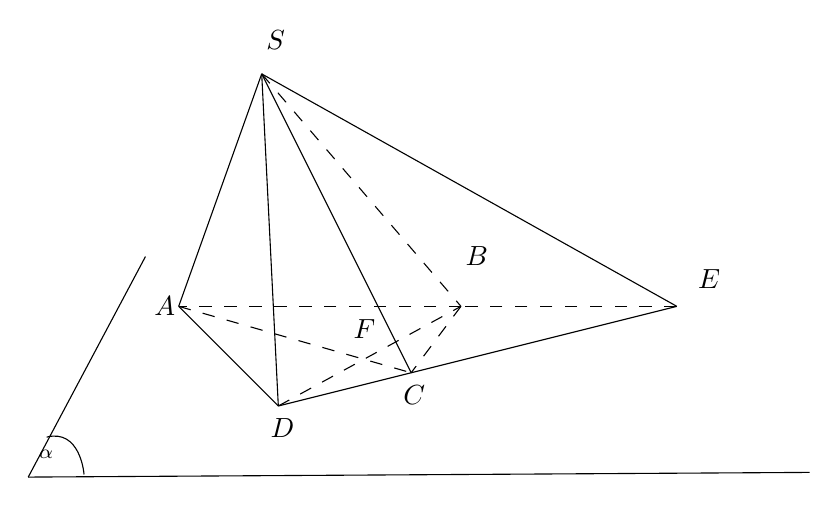
\begin{tikzpicture}[x=0.75pt,y=0.75pt,yscale=-1,xscale=1]
					\draw (143.51,234.26) --  (520,232);
					\draw  (200,128) -- (143.51,234.26);
					\draw (152.38,215).. controls (168.38,211) and (170.38,232)..  (170.38,233);
					\draw [dash pattern={on 4.5pt off 4.5pt}] (352,152) -- (216,152); 
					\draw (216,152)  -- (264,200);
					\draw  (328,184) -- (264,200);
					\draw [dash pattern={on 4.5pt off 4.5pt}]  (352,152) -- (328,184);
					\draw (456,152) --  (328,184);
					\draw [dash pattern={on 4.5pt  off 4.5pt}] (456,152) -- (352,152);
					\draw (256,40) -- (216,152); 
					\draw (256,40)  -- (264,200);
					 \draw (256,40) -- (328,184);
					\draw [dash pattern={on 4.5pt off 4.5pt}] (256,40) --  (352,152);
					\draw  (256,40) -- (456,152);
					 \draw [dash pattern={on 4.5pt off 4.5pt}] (216,152) -- (328,184);
					\draw [dash pattern={on 4.5pt  off 4.5pt}] (264,200) -- (352,152);
					\draw (147.38,220) node  [anchor=north west][inner sep=0.75pt] [font=\scriptsize] [align=left] {$\alpha$};
					\draw (257,18) node  [anchor=north west][inner sep=0.75pt] [align=left] {$S$};
					\draw (203,146) node [anchor=north west][inner sep=0.75pt]  [align=left] {$A$};
					\draw (353,122) node [anchor=north west][inner sep=0.75pt]  [align=left] {$B$};
					\draw (323,189) node [anchor=north west][inner sep=0.75pt] [align=left]  {$C$};
					 \draw (259,205) node [anchor=north west][inner sep=0.75pt] [align=left] {$D$};
					\draw (465,133) node [anchor=north west][inner  sep=0.75pt] [align=left] {$E$};
					\draw (299,157) node [anchor=north west][inner  sep=0.75pt] [align=left] {$F$};
				\end{tikzpicture}
		\end{center}
		ta  có $\heva{&S\in (SAB)\\&S\in (SCD)}$
		$\Rightarrow  S$ là điểm chung thứ 1.\\
		$\heva{&E\in AB, AB\subset (SAB)\Rightarrow S\in (SAB)\\&E\in CD, CD\subset (SCD)\Rightarrow E\in (SCD)}\Rightarrow  E$ là điểm chung thứ 2.\\
		Do đó $SE$ là giao tuyến  của 2 mặt phẳng $SCD$ và $SAB$.\\
	 }
\end{ex}

% nguồn: Ok_TracNghiemLop11_Lan1
\begin{ex}%[1H4H1-3]%[ma:59b8073a]
	Cho tứ diện $ABCD$. Gọi $M$, $N$ lần lượt là trung điểm của $AC$,  $CD$. Giao tuyến của hai mặt phẳng $\left(MBD\right)$ và $\left(ABN\right)$ là
	\choice 
		{Đường thẳng  $MN$}
		 {\True Đường thẳng $BG$ ($G$ là trọng tâm tam giác $ACD$)}
		{Đường  thẳng $AM$}
		{Đường thẳng $AN$ ($N$ là trực tâm  tam giác $ACD$)}
	 \loigiai{
		\begin{center}
			\begin{tikzpicture}[scale=1,font=\footnotesize,line join=round,line cap=round,>=stealth]
					\path 
						(-2,0) coordinate (B) 
						(-1,-2) coordinate (C) 
						(3,0)  coordinate (D)
						($(B)+(2,3)$) coordinate  (A)
						($(A)!0.5!(C)$) coordinate (M) 
						($(C)!0.5!(D)$) coordinate  (N);
					\coordinate (G) at (intersection of  A--N and D--M);
					\draw (A)--(B) 
						(A)--(C) 
						(A)--(D) 
						 (B)--(C)--(D)
						(B)--(M)--(D) 
						 (A)--(N);
					\draw [dashed] (N)--(B)--(D); 
					\foreach \x/\g in {A/90,B/180,C/-90,D/0,M/150,N/-90,G/50} \draw[fill](\x)  circle (.5pt)
						 ($(\x)+(\g:3mm)$) node[scale=1]{$\x$};
				\end{tikzpicture}
		\end{center}
		Gọi $G$ là trọng tâm của tam giác $ACD$.\\ 
		Ta  có
		$\left.\begin{array}{l}
		B\in\left(BDM\right)\\ 
		B\in\left(ABN\right) 
\end{array}\right\}\Rightarrow B\in\left(BDM\right)\cap\left(ABN\right)$.\\
Và 
$\left.\begin{array}{l}
AN\subset\left(ABN\right)\\ 
 DM\subset\left(BDM\right)\\
DM\cap AN=\left\{G\right\} 
\end{array}\right\}G\in\left(BDM\right)\cap\left(ABN\right)$.\\
Suy  ra $\left(BDM\right)\cap\left(ABN\right)=BG$.
 }
\end{ex}

% nguồn: Ok_TracNghiemLop11_Lan1
\begin{ex}%[1H4H1-3]%[ma:4959b1f8]
	Cho hình chóp tứ giác $S.ABCD$ có đáy là hình thang $( AD\parallel BC)$. Gọi $H$ là trung điểm $AB$. Giao tuyến của hai mặt phẳng $( SHD)$ và  $( SAC)$ là
	 \choice
		{ \True $SI$ ($I$  là giao điểm của $HD$ và $AC$)}
		{ $SK$ ($K$ là giao điểm  của $AB$ và $CD$)}
		{ $SO$  ($O$ là giao điểm của $AC$ và $BD$)}
		{ $SA$} 
	\loigiai{ 
	\immini{\begin{itemize}
		\item  $S$ là điểm chung thứ nhất của $( SHD)$ và $( SAC)$.
		\item Gọi $I$ là giao điểm của $AC$ và $HD$ nên $I\in AC$,  $I\in HD$ do đó $I$ là điểm chung thứ hai $( SHD)$ và $( SAC)$.
	\end{itemize}
	Vậy giao tuyến của hai mặt phẳng $( SHD)$ và $( SAC)$  là $SI$.}
	{\begin{tikzpicture}[scale=0.6,font=\footnotesize,line join=round,line cap=round,>=stealth]
		 \def\bc{5}
		 \def\ba{3.5}
		 \def\h{5}
		\def\gocB{100} 
		\coordinate  (B) at (0,0);
		\coordinate (A)  at (\gocB:\ba);
		\coordinate (C) at  (\bc,0);
		 \coordinate (D) at ($(A)+(0:2*\bc)$);
		\coordinate (S) at ($(A)+(60:\h)$); 
		\coordinate (H)  at ($(A)!0.5!(B)$);
		\coordinate (I) at (intersection of C--A and  H--D);
		 \draw (B)--(C)--(D)--(S)--cycle (S)--(A)--(B)
			(H)--(S)--(C); 
		\draw[dashed]  (C)--(A)--(D)
			 (D)--(H)
			 (S)--(I);
		\foreach \p/\i in  {A/180,B/-90,D/0,C/-90,S/90,I/-90,H/180}
		\fill (\p) circle (1pt)  node[shift={(\i:3mm)}]{$\p$};
	\end{tikzpicture}
}} 
\end{ex}

% nguồn: Ok_TracNghiemLop11_Lan1
\begin{ex}%[1H4H1-3]%[ma:79325f8c]
	 -
	Cho hình chóp $ S.ABCD$. Gọi $ O$ là giao điểm của $ AC$ và $ BD$. Giao tuyến của hai mặt phẳng $\left(SAC\right)$  và $\left(SBD\right)$ là đường thẳng
	 \choice
		{$  SM$}
		{\True $ SO$} 
		 {$ SN$}
		{$  MN$}
	\loigiai{ 
		\begin{center}
			\tikzset{every picture/.style={line width=0.75pt}} 
			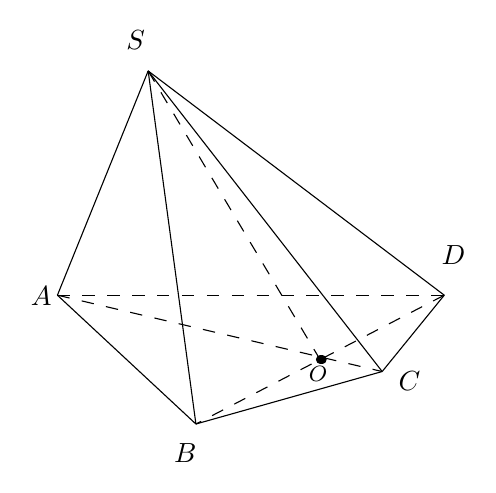
\begin{tikzpicture}[x=0.75pt,y=0.75pt,yscale=-1,xscale=1]
					\draw [dash pattern={on 4.5pt off 4.5pt}] (242.11,141.19) -- (428.49,141.19); 
					\draw  (242.11,141.19) -- (308.84,203.26);
					\draw (308.84,203.26)  -- (398.58,177.97);
					\draw (428.49,141.19) --  (398.58,177.97);
					\draw (285.83,33.14) --  (242.11,141.19);
					 \draw (285.83,33.14) -- (308.84,203.26);
					\draw (285.83,33.14) -- (398.58,177.97); 
					\draw  (285.83,33.14) -- (428.49,141.19);
					\draw [dash pattern={on 4.5pt  off 4.5pt}] (428.49,141.19) -- (308.84,203.26);
					\draw [dash pattern={on 4.5pt off 4.5pt}] (242.11,141.19) -- (398.58,177.97); 
					\draw [dash  pattern={on 4.5pt off 4.5pt}] (285.83,33.14) -- (368.67,172.23);
					\draw [line width=3] [line join = round][line cap =  round] (368.67,172.23).. controls (369.05,172.23) and (369.43,172.23).. (369.82,172.23);
					 \draw (274.08,12.57) node [anchor=north west][inner sep=0.75pt] [align=left] {$S$};
					\draw  (228.05,135.56) node [anchor=north west][inner sep=0.75pt] [align=left] {$A$};
					\draw (297.09,211.43) node [anchor=north west][inner sep=0.75pt]  [align=left] {$B$};
					\draw (405.24,176.95) node [anchor=north west][inner sep=0.75pt] [align=left]  {$C$};
					\draw (425.95,116.02) node  [anchor=north west][inner sep=0.75pt] [align=left] {$D$};
					\draw (362,174) node [anchor=north  west][inner sep=0.75pt] [font=\footnotesize] [align=left] {$O$};
				\end{tikzpicture}
		\end{center}
		$\heva{&S\in (SAC) \\&S\in (SBD)}\Rightarrow S$ là điểm chung thứ nhất.\\ 
		 $\heva{
		&O\in  AC\subset\left(SAC\right)\\
		&O\in BD\subset\left(SBD\right)}$ $ \Rightarrow O$ là điểm chung  thứ hai.\\
		 Vậy $\left(SAC\right)\cap\left(SBD\right)=SO$.
	 }
\end{ex}

% nguồn: Ok_TracNghiemLop11_Lan1
\begin{ex}%[1H4H1-3]%[ma:adc9caf6]
	Cho hình chóp $ S.ABCD$ có đáy là  hình bình hành. Gọi $M$, $N$ lần lượt là trung điểm của $AD$ và $BC$. Giao tuyến của hai mặt phẳng $(SMN)$ và $(SAC)$ là
	 \choice
		{$ SD$} 
		{\True $ SO$ với  $O$ là tâm hình bình hành $ABCD$}
		{$SG$ với $G$ là trung  điểm của $AB$}
		{$ SF$ với $F$ là trung điểm  $CD$}
	 \loigiai{
	 \immini{
		Ta có $S$  là điểm chung của hai mặt phẳng $(SMN)$ và $(SAC)$.\\
		Gọi $O$ là tâm của hình bình hành $ABCD$ nên $AC\cap  MN=O$\\
		Ta có  $\heva{&O\in MN,~MN\in (SMN) \Rightarrow O \in (SMN)\\ & OI \in AC,~AC\in (SAC)\Rightarrow O \in (SAC).}$\\
		Suy ra, $O$ cũng là điểm chung của hai  mặt phẳng $(SMN)$ và $(SAC)$.\\
		Vậy $SO$ là giao tuyến của hai mặt  phẳng $(SMN)$ và $(SAC)$.}
		 {
		\begin{tikzpicture}[scale=0.8,font=\footnotesize,line join=round,line cap=round]
				\coordinate (A) at (0,0); 
				\coordinate  (B) at (-2,-1.5);
				 \coordinate (D) at (5,0);
				\coordinate (C) at  ($(B)+(D)-(A)$);
				\coordinate (M) at ($(A)!0.5!(D)$); 
				\coordinate (N)  at ($(B)!0.5!(C)$);
				\coordinate (O) at ($(A)!0.5!(C)$); 
				\coordinate  (S) at (0,4);
				\draw (S)--(B)--(C)--(D)--(S)--(C) 
					 (S)--(N);
				 \draw[dashed] (B)--(A)--(D)
					(S)--(A) 
					(B)--(D) 
					(S)--(M)--(N) 
					 (A)--(C)
					(S)--(O); 
				\foreach \i/\g in  {S/90,A/160,B/-90,C/-90,D/0,M/60,N/-90,O/-90}{\draw[fill](\i) circle (1pt)
					 ($(\i)+(\g:3mm)$) node {$\i$};}
			\end{tikzpicture}
		 }
	 }
\end{ex}

% nguồn: Ok_TracNghiemLop11_Lan1
\begin{ex}%[1H4H1-3]%[ma:4ee4d722]
	
	Cho hình chóp $  S.ABCD$, đáy $ ABCD$ là hình bình hành $ ABCD$ tâm $ O$. Giao tuyến của hai mặt phẳng $\left(SAC\right)$ và $\left(SAD\right)$ là
	\choice 
		 {$SO$}
		 {$SD$}
		{\True $SA$} 
		 {$SB$}
	\loigiai{ 
		Ta có $\heva{&A\in (SAC)\\&A\in (SAD)}$ $\Rightarrow A$  là điểm chung thứ nhất.\\
		$\heva{&A\in (SAC)\\&A\in (SAD)}$ $\Rightarrow A$ là điểm chung thứ  2.\\
		Do đó $SA$ là giao tuyển của 2 mặt phẳng  $\left(SAC\right)$ và $\left(SAD\right)$.
	 }
\end{ex}

% nguồn: Ok_TracNghiemLop11_Lan1
\begin{ex}%[1H4H1-3]%[ma:38c61945]
	
	Cho tứ diện $ ABC{\rm{D}}$,  $ G$ là trọng tâm tam giác $ BCD$. Giao tuyến của $\left(ACD\right)$ và $\left(GAB\right)$ là
	 \choice
		 {$ AM$ (với $ M$ là trung điểm $ AB$)}
		{\True $  AN$ (với $ N$ là trung điểm $ CD$)}
		{$ AK$ (với $ K$ là hình chiếu của $ C$ trên $ BD$)} 
		{$ AH$ (với $ H$ là hình chiếu của $  B$ trên $CD$)}
	\loigiai{ 
		\begin{center}
			\tikzset{every picture/.style={line  width=0.75pt}}
			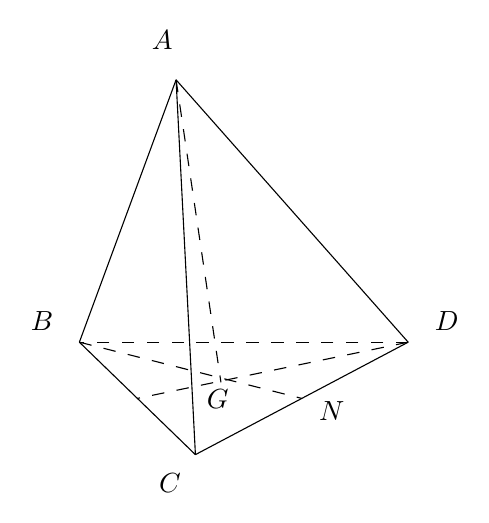
\begin{tikzpicture}[x=0.75pt,y=0.75pt,yscale=-1,xscale=1]
					\draw [dash pattern={on 4.5pt  off 4.5pt}] (378.21,169.61) -- (219.79,169.61);
					\draw (219.79,169.61)  -- (275.7,223.79);
					\draw (266.38,43.21) --  (219.79,169.61);
					\draw  (266.38,43.21) -- (275.7,223.79);
					\draw (266.38,43.21) -- (378.21,169.61); 
					 \draw [dash pattern={on 4.5pt off 4.5pt}] (219.79,169.61) -- (326.96,196.7);
					 \draw (378.21,169.61) -- (275.7,223.79);
					\draw [dash pattern={on 4.5pt  off 4.5pt}] (378.21,169.61) -- (247.75,196.7);
					\draw [dash pattern={on 4.5pt  off 4.5pt}] (266.38,43.21) -- (288,189);
					\draw  (253.4,18.35) node [anchor=north west][inner sep=0.75pt] [align=left] {$A$};
					\draw (195.15,153.78) node [anchor=north west][inner sep=0.75pt]  [align=left] {$B$};
					 \draw (256.97,231.65) node [anchor=north west][inner sep=0.75pt] [align=left] {$C$};
					\draw (389.76,153.78) node  [anchor=north west][inner sep=0.75pt] [align=left] {$D$};
					\draw (280,191) node [anchor=north  west][inner sep=0.75pt] [align=left] {$G$};
					\draw (334,197) node [anchor=north west][inner sep=0.75pt]  [align=left] {$N$};
				\end{tikzpicture}
		\end{center}
		Vì $G$ là trọng tâm tam giác $BCD$ nên gọi $N$ là  trung điểm của $CD$.\\
		 $\heva{&N\in BG, BG\subset (ABG)\Rightarrow N\in (ABG)\\&N \in CD \Rightarrow N\in (ACD)}\Rightarrow N$ là điểm chung thứ nhất.\\
		$\heva{&A\in (ABG)\\&A\in (ACD)}$  $\Rightarrow A$ là điểm chung thứ hai\\.
	Ta thấy $\left(GAB\right)$ chính là mặt phẳng $\left(ANB\right)$. Suy  ra giao tuyến của $\left(GAB\right)$ với $\left(AC{\rm{D}}\right)$ chính là $ AN$.}
\end{ex}

% nguồn: Ok_TracNghiemLop11_Lan1
\begin{ex}%[1H4H1-3]%[ma:7cb230f6]
	Cho tứ diện $ABCD$ và điểm  $M$ thuộc miền trong của tam giác $ACD$. Gọi $I$ và $J$ lần lượt là hai điểm trên cạnh $BC$ và $BD$ sao cho $IJ$ không song song với $CD$. Gọi $H$, $K$ lần lượt là giao điểm cùa $IJ$ với $CD$ của $MH$ và $AC$. Giao tuyến của hai mặt phẳng $(ACD)$ và $(IJM)$ là
	 \choice
		 {$KI$}
		{$KJ$} 
		 {$MI$}
		{\True $MH$} 
	\loigiai{ 
		\begin{center}
			\begin{tikzpicture}[scale=1,font=\footnotesize,line join=round,line cap=round,>=stealth]
					\path 
						(-2,-2) coordinate  (B)
						(3,-2) coordinate (C) 
						(0,-0.5)  coordinate (D)
						($(D)+(85:3)$)  coordinate (A)
						($(D)+(10:1.3)$) coordinate (M) 
						($(B)!0.4!(C)$)  coordinate (I)
						($(B)!0.8!(D)$) coordinate (J) 
						($(C)!1.5!(D)$) coordinate (x) 
						($(I)!1.5!(J)$)  coordinate (y);
					\coordinate (H) at (intersection of C--x and  I--y);
					\coordinate  (z) at ($(H)!1.5!(M)$);
					\coordinate (K) at (intersection of A--C and  H--z);
					\draw (A)--(B) 
						(A)--(C) 
						(B)--(C); 
					 \draw[dashed] (A)--(D)
						 (B)--(D)--(C)
						(I)--(H)--(K) 
						(J)--(M)--(I); 
					\foreach \x/\g  in {A/90,B/180,C/-90,D/-90,M/90,I/-90,J/180,H/90,K/0} \draw[fill](\x) circle (.5pt)
						 ($(\x)+(\g:3mm)$) node[scale=1]{$\x$};
				\end{tikzpicture}
		\end{center}
		Ta có điểm $M$ thuộc miền trong của tam giác $ACD$ và $H$ là giao điểm cùa $IJ$ với $CD$ nên hai mặt phẳng $(ACD)$  và $(IJM)$ có hai điểm chung $M$ và $H$ nên có giao tuyến là $MH$.
	 }
\end{ex}

% nguồn: Ok_TracNghiemLop11_Lan1
\begin{ex}%[1H4H1-3]%[ma:c37e56be]
	Cho hình chóp $S.ABCD$  có đáy $ABCD$ là hình thang với đáy lớn $AD$. Gọi $M$ là trung điểm của $CD$. Giao tuyến của hai mặt phẳng $(MSB)$ và $(SAC)$ là đường thẳng
	 \choice
		{\True $SI$ với $I$ là giao điểm của $AC$ và  $BM$}
		{$SP$ với $P$ là giao điểm của $AB$  và $CD$}
		{$SI$ với $J$ là  giao điểm của $AM$ và $BD$}
		{$SO$ với $O$ là giao điểm của $AC$ và $BD$} 
	 \loigiai{
	 \immini{
		 Ta có $S$ là điểm chung của hai mặt phẳng $(SAC)$ và $(SBM)$.\\
		Trong $(ABCD)$ gọi $I=AC\cap  BM$.\\
		Ta có $\heva{&I\in AC,~AC\in (SAC)  \Rightarrow I \in (SAC)\\ & I \in BM,~BM\in (SBM)\Rightarrow I \in (SBM).}$\\
		Suy  ra, $I$ cũng là điểm chung của hai mặt phẳng $(SAC)$ và $(SBM)$.\\
		Vậy $SI$ là giao tuyến của hai mặt phẳng  $(SAC)$ và $(SBM)$.
		 }{
		\begin{tikzpicture}[scale=0.8,font=\footnotesize,line join=round,line cap=round]
				\coordinate  (A) at (0,0);
				\coordinate (B) at  (0.5,-2);
				\coordinate (C) at  (3.5,-2);
				\coordinate (D)  at (6,0);
				\coordinate (M) at ($(C)!0.5!(D)$); 
				 \coordinate (S) at (2,4);
				\coordinate (I) at (intersection of A--C and  B--M);
				\draw  (S)--(A)--(B)--(C)--(D)--(S)--(B)
					 (S)--(C)
					 (S)--(M);
				 \draw[dashed] (A)--(D)
					(B)--(M) 
					 (A)--(C)
					 (S)--(I);
				\foreach \i/\g in {S/90,A/180,B/-90,C/-90,D/0,M/-60,I/-90}{\draw[fill](\i)  circle (1pt)
					($(\i)+(\g:3mm)$) node {$\i$};} 
			\end{tikzpicture}
		} 
	 }
\end{ex}

% nguồn: Ok_TracNghiemLop11_Lan1
\begin{ex}%[1H4H1-3]%[ma:38f12600]
	Cho hình chóp $ S.ABCD$ có đáy là hình  thang $ ABCD\,(AB\parallel CD)$. Khẳng định nào sau đây {\bf sai}?
	\choice 
		{Hình chóp $ S.ABCD$  có 4 mặt bên}
		{Giao tuyến của hai mặt phẳng $\left(SAC\right)$  và $\left(SBD\right)$ là $SO$ ($O$ là giao điểm của $AC$ và $BD$)}
		{Giao tuyến của hai mặt phẳng $\left(SAD\right)$ và $\left(SBC\right)$ là $SI$ ($I$ là giao điểm của  $AD$ và $BC$)}
		{\True Giao tuyến của hai mặt phẳng $\left(SAB\right)$  và $\left(SAD\right)$ là đường trung bình của $ ABCD$}
	 \loigiai{
		Ta có $\heva{&A\in (SAB)\\&A\in (SAD)}$ $\Rightarrow  A$ là điểm chung thứ nhất.\\
		$\heva{&A\in (SAB)\\&A\in (SAD)}$ $\Rightarrow  A$ là điểm chung thứ 2.\\
	Do đó $SA$ là giao tuyển của 2 mặt phẳng $\left(SAB\right)$ và $\left(SAD\right)$.  }
\end{ex}

% nguồn: Ok_Toan11_TracNghiem_Lan2
\begin{ex}%[1H4Y1-3]%[ma:e598ffdc]
	Cho $4$ điểm $A,B,C,D$ không cùng nằm trên một mặt phẳng. Trên $AB,AD$ lần lượt lấy $2$ điểm $M,N$  sao cho $MN$ cắt $BD$ tại $I$. Giao tuyến của mặt phẳng $(ABD)$ và $(ADC)$ là
	\choice 
		{\True  $AD$}
		 {$DB$}
		{$MN$} 
		 {$CI$}
	 \loigiai{
		\begin{center}
			\begin{tikzpicture}[scale=1,font=\footnotesize,line join=round,line cap=round,>=stealth]
					 \def\ac{4.5}
					\def\ab{3} 
					 \def\as{4}
					\def\gocA{30} 
					\coordinate[label=below left:$D$] (D) at  (0,0);
					\coordinate[label=right:$C$] (C) at (\ac,0); 
					\coordinate[label=below left:$B$] (B)  at (-\gocA:\ab);
					\coordinate[label=above:$A$] (A) at  (65:\as);
					 \coordinate[label=right:$M$] (M) at ($(A)!0.3!(B)$);
					\coordinate[label=above left:$N$]  (N) at ($(A)!0.6!(D)$);
					\coordinate[label=left:$I$] (I) at  (intersection of B--D and N--M);
					\draw (A)--(D)--(B)--(C)--cycle (A)--(B) 
						(D)--(I)--(M); 
					 \draw[dashed] (D)--(C);
					\foreach \diem in {A,B,C,D,I,M,N}\fill (\diem)  circle (1pt);
				\end{tikzpicture}
		\end{center}
	 Hai mặt phẳng $(ABD)$ và $(ADC)$ có điểm $A$ và $D$ chung nên giao tuyến là $AD$}
\end{ex}

% nguồn: Ok_Toan11_TracNghiem_Lan2
\begin{ex}%[1H4Y1-3]%[ma:2720ff17]
	Cho hình chóp $S.ABCD$ với  $ABCD$ là hình bình hành. Khi đó giao tuyến của hai mặt phẳng $(SAC)$ và $(SAD)$ là
	 \choice
		{Đường thẳng  $SC$}
		{Đường thẳng  $SB$}
		{Đường thẳng  $SD$}
		{\True Đường  thẳng $SA$}
	\loigiai{ 
	Ta thấy $(SAC)\cap  (SAD)=SA$.}
\end{ex}

% nguồn: Ok_Toan11_TracNghiem_Lan2
\begin{ex}%[1H4Y1-3]%[ma:c248e17f]
	Cho hình chóp tứ giác $S.ABCD$ Giao tuyến của hai mặt phẳng $(SAB)$  và $(SBC)$ là
	\choice 
		 {$SA$}
		{\True  $SB$}
		 {$SC$}
		 {$AC$}
	 \loigiai{
	Ta có: $\heva{&  S\in (SAB)\cap (SBC) \\ & B\in (SAB)\cap (SBC)}\Rightarrow SB$ là giao tuyến của hai mặt phẳng $(SAB)$ và $(SBC)$.}
\end{ex}

% nguồn: Ok_Toan11_TracNghiem_Lan2
\begin{ex}%[1H4Y1-3]%[ma:b5574d57]
	Cho bốn điểm $A,B,C,D$ không đồng phẳng. Gọi $I,K$ lần lượt là trung  điểm hai đoạn thẳng $AD$ và $BC$. $IK$ là giao tuyến của cặp mặt phẳng nào sau đây ?
	 \choice
		 {$(IBC)$ và $(KBD)$}
		{$(IBC)$ và $(KCD)$} 
		{\True $(IBC)$  và $(KAD)$}
		{$(ABI)$ và $(KAD)$} 
	 \loigiai{
		\begin{center}
			\begin{tikzpicture}[scale=1,font=\footnotesize,line join=round,line cap=round,>=stealth]
					\def\ac{4} 
					\def\ab{2} 
					 \def\as{3.5}
					 \def\gocA{50}
					\coordinate[label=left:$A$]  (A) at (0,0);
					\coordinate[label=right:$C$] (C)  at (\ac,0);
					 \coordinate[label=below left:$B$] (B) at (-\gocA:\ab);
					\coordinate[label=above:$D$] (S)  at (70:\as);
					\coordinate[label=left:$I$] (I) at  ($(A)!0.5!(S)$);
					 \coordinate[label=below right:$K$] (K) at ($(B)!0.5!(C)$);
					\draw (A)--(B)--(C)--(S)--cycle  (S)--(B)
						 (I)--(B);
					\draw[dashed]  (A)--(C)
						(A)--(K)--(I)--(C); 
					\foreach \diem in {A,B,C,S,K,I}\fill (\diem) circle (1pt); 
				\end{tikzpicture}
		\end{center}
		 $\heva{& I\in AD\subset (KAD) \\ & I\in (IBC)}$ $\Rightarrow I$ là điểm chung thứ nhất của hai mặt phẳng $(IBC)$ và $(KAD)$.\\
		$\heva{& K\in BC\subset (IBC) \\ & K\in (KAD)}$$\Rightarrow K$ là điểm chung thứ hai của hai mặt  phẳng $(IBC)$ và $(KAD)$.\\
		 Vậy $(IBC)\cap (KAD)=IK$.
	 }
\end{ex}


%%%%%%%%%%%%%%%% ĐÚNG/SAI %%%%%%%%%%%%%%%%

% nguồn: Ok_dungsai_lop11_Lan1
\begin{ex}%[1H4N1-3]%[ma:c35c0d49]
 Cho hình chóp $S.ABCD$  có đáy là hình bình hành $ABCD$. Gọi $M$ là một điểm thuộc miền trong của tam giác $BCD$, $N$ thuộc $SM$.
  \choiceTF
  {\True $AB$ là  giao tuyến của $\left(SAB\right)$ và $\left(ABD\right)$}
  {Giao tuyến của $\left(MND\right)$ và $\left(ABCD\right)$ không cắt  $BC$}
  {Giao tuyến của $\left(SBC\right)$ và  $\left(SAD\right)$ là đường thẳng song song với $BD$}
  {\True Gọi $P=CM\cap BD,\, Q=CN\cap SP$. Khi đó $DQ$ là giao tuyến của $\left(NCD\right)$ và  $\left(SBD\right)$}
 \loigiai{ 
  \begin{center}
   \begin{tikzpicture}[>=stealth,line join=round,line cap = round,scale=1,font=\footnotesize]
      \def\ac{5}
     \def\ab{4} 
     \def\h{4} 
     \def\gocA{-120} 
      \path
       (0,0) coordinate (B)
      (\gocA:\ab) coordinate (A) 
      (\ac,0)  coordinate (C)
       ($(A)+(C)-(B)$) coordinate (D)
      (-0.5,\h) coordinate (S) 
       ($(B)!3/5!(D)$) coordinate (P)
       ($(C)!2/5!(P)$) coordinate (M)
       ($(S)!2/3!(M)$) coordinate (N)
      (intersection of C--N and S--P) coordinate (Q) 
      (intersection of B--C and D--M) coordinate  (E);
      \foreach \p/\q in {S/90,A/180,B/180,C/0,D/-90,N/45,M/-40,Q/180,E/-45,P/180}
     \fill[black] (\p)  circle (1.0pt) node[shift={(\q:3.5mm)}]{$\p$};
     \draw (S)--(A)--(D)--(S)--(C)--(D); 
     \draw[dashed] (A)--(B)--(C) 
       (S)--(B)--(D)
       (C)--(P)--(Q)--cycle (D)--(N)--(E)--cycle (M)--(S)--(Q);
    \end{tikzpicture}
  \end{center}
  \begin{itemchoice}
   \itemch \textbf{Đúng}. Ta có $AB$  là giao tuyến của $\left(SAB\right)$ và $\left(ABD\right)$.
   \itemch \textbf{Sai}. $\left(MND\right)\cap\left(ABCD\right)=MD$ mà $MD\cap BC=E$ nên giao tuyến của $\left(MND\right)$ và  $\left(ABCD\right)$ cắt $BC$ tại $E$.
   \itemch \textbf{Sai}. $S\in\left(SBC\right)\cap\left(SAD\right)$ và $BC \parallel AD$ nên giao tuyến của $\left(SBC\right)$  và $\left(SAD\right)$ là đường thẳng đi qua $S$ và song song với $BC$ và $AD$.
   \itemch \textbf{Đúng}. $D\in\left(NCD\right)\cap\left(SBD\right)$.\\ 
    $Q=CN\cap SP\Rightarrow\heva{
   &Q\in CN,\,CN\subset\left(NCD\right)\\ 
   &Q\in  SP,\,SP\subset\left(SBD\right)}
   \Rightarrow Q\in\left(NCD\right)\cap\left(SBD\right)$ .\\ 
   $\Rightarrow DQ=\left(NCD\right)\cap\left(SBD\right)$. 
  \end{itemchoice}
 } 
\end{ex}

% nguồn: Ok_dungsai_lop11_Lan1
\begin{ex}%[1H4N1-3]%[ma:8b4b5825]
 Cho hình  chóp $S.ABCD$, gọi hai điểm $M$, $N$ lần lượt là trung điểm $SD$, $CD$.
  \choiceTF
  {\True $CD$ là giao tuyến  của hai mặt phẳng $\left(SCD\right)$ và $\left(ABCD\right)$}
  {\True Gọi $O$ là giao điểm của $AC$ và $BD$, $SO$ là giao  tuyến của hai mặt phẳng $\left(SAC\right)$ và $\left(SBD\right)$}
  {Giả sử $AB$ không song song $CD$ Gọi $P$ là giao điểm của $AC$ và $BN$, $SP$ là giao tuyến của hai mặt phẳng $\left(SAB\right)$ và  $\left(SCD\right)$}
  {Giao điểm của $SA$ và mặt  phẳng$\left(BMN\right)$ là giao điểm của $SA$ và $BN$}
 \loigiai{ 
  \begin{tikzpicture}[>=stealth,line join=round,line cap = round,scale=1,font=\footnotesize]
     \def\ad{6}
    \def\ab{2} 
     \def\h{4}
     \def\gocA{-80}
     \path
     (0,0)  coordinate (A)
     (\gocA:\ab) coordinate (B) 
     ($(B)+(3,-1)$) coordinate  (C)
     (\ad,0) coordinate (D) 
     (2.5,\h) coordinate  (S)
     ($(C)!0.5!(D)$)  coordinate (N)
      ($(S)!0.5!(D)$) coordinate (M)
     (intersection of B--N and A--C) coordinate  (P)
     ($(P)+(S)-(C)$) coordinate (P') 
      (intersection of S--A and P--P') coordinate (Q);
     \foreach \p/\q in {S/90,A/180,B/-90,C/-90,D/0,N/-90,M/0,P/-90,Q/180}
    \fill[black] (\p) circle (1.0pt) node[shift={(\q:3.5mm)}]{$\p$}; 
    \draw  (S)--(D)--(C)--(S)--(A)--(B)--(C)
     (M)--(N) 
      (S)--(B)
      (B)--(Q);
    \draw[dashed] (A)--(D) 
     (B)--(N) 
      (A)--(C)
     (S)--(P) 
      (B)--(M)
      (Q)--(M)
     (P)--(Q); 
   \end{tikzpicture}
  \begin{itemchoice}
   \itemch \textbf{Đúng}. Ta có $ C $ là điểm chung thứ nhất và $ D $ là điểm  chung thứ hai.\\
   Vậy CD là giao tuyến  của hai mặt phẳng $\left(SCD\right)$ và $\left(ABCD\right)$.
   \itemch \textbf{Đúng}. Ta có $ S $ là điểm chung thứ nhất và $ O $ là giao điểm của $ AC$ và $ BD  $, suy ra $ O $ là điểm chung thứ hai.\\
   Vậy  $ SO $ là giao tuyến của hai mặt phẳng $\left(SAC\right),\left(SBD\right)$.
   \itemch \textbf{Sai}. Ta  có $ S $ là điểm chung thứ nhất.\\
   Gọi $ I $ là giao điểm của $  AB $ và $ CD$, suy ra $ I $ là điểm chung thứ hai.\\
   Vậy $ SI $ là giao tuyến của hai  mặt phẳng $\left(SAC\right)$, $\left(SBD\right)$.
   \itemch \textbf{Sai}.  Do $ SA $ và $ BN $ là hai đường thẳng chéo nhau nên chúng không có điểm chung.
  \end{itemchoice}
 } 
\end{ex}

% nguồn: Ok_dungsai_lop11_Lan2
\begin{ex}%[1H4N1-3]%[1H4V1-3]%[ma:0cc4e291]
	Cho hình chóp $S.ABCD$ có đáy $ABCD$ là một hình bình hành tâm ${O}$.  Gọi $I$, $K$ lần lượt là trung điểm của $SB$ và $SD$. Khi đó:
	\choiceTF 
		 {\True $SO$ là giao tuyến của $(SAC)$ và $(SBD)$}
		{Giao điểm $J$ của $SA$ với $(CKB)$ thuộc đường  thẳng đi qua $K$ và song song với $DC$}
		{\True Giao tuyến của $(OIA)$ và $(SCD)$ là đường thẳng đi qua  $C$ và song song với $SD$}
		{\True  $CD\parallel IJ$}
	 \loigiai{
		\begin{center}
			\begin{tikzpicture}[line cap=round,line join=round,font=\footnotesize]
					 \path
						 (0:0) coordinate (A)
						 (0:4) coordinate (D)
						++(235:2.5) coordinate  (C)
						 ($(A)+(C)-(D)$) coordinate (B)
						($(A)+(80:4)$) coordinate  (S)
						(intersection of A--C and B--D) coordinate (O) 
						(barycentric cs:S=1,B=1)  coordinate (I)
						(barycentric cs:S=1,D=1) coordinate (K) 
						(barycentric cs:S=1,A=1) coordinate  (J)
						($(S)+(C)-(D)$) coordinate (Cy); 
					\draw[dashed] (B)--(A)--(D)--cycle  (C)--(A)--(S)
						 (S)--(O)
						(A)--(I)--(J)--(K)--(B) 
						 (C)--(I)--(O);
					 \draw[] (B)-- (C)--(D)
						 (B)--(S)
						 (C)--(S)
						(D)--(S) 
						 ($(C)!-.5cm!(Cy)$)--(C)--(Cy) node[right]{$y$}
						 (K)--($(K)!-1cm!(J)$) node[above]{$x$};
					\foreach \x/\y  in {A/180,B/210,C/-90,D/0,S/90,O/-90,I/180,K/80,J/180}
					\fill[black] (\x) circle (1pt) 
						($(\y:3mm)+(\x)$) node {$\x$}; 
				\end{tikzpicture}
		\end{center}
		\begin{itemchoice}
			\itemch Đúng.\\ 
			$\heva{ 
			&O\in AC\subset (SAC)\\ 
			&O\in BD\subset  (SBD)}$
			$\Rightarrow O\in (SAB)\cap (SCD)$\\ 
			$S\in (SAB)\cap (SCD) \Rightarrow SO=(SAC)\cap (SBD)$. 
			\itemch  Sai.\\
			Tứ  giác $ABCD$ là hình bình hành nên $AB\parallel CD;\, AD\parallel BC$.\\
			Ta  có: $\heva{
			&AD\parallel  CB\\
			 &AD\subset (SAD)\\
			 &BC\subset (SBC)\\
			&K\in (KBC)\cap (SAD)}$ 
			 $\Rightarrow
			 \heva{
			&Kx=(KBC)\cap (SAD)  \\
			&Kx\parallel  AD\parallel BC.}$\\
			Trong  $(SAD)$ gọi $J=Kx \cap SA$, có $\Rightarrow
			\heva{ 
			&J\in SA  \\
			&J\in  Kx\subset (BKC)}$
			 $\Rightarrow J=SA\cap (BKC)$.
			\itemch Đúng.\\ 
			Có ${O I}$ là đường  trung bình của $\Delta SBD\Rightarrow OI\parallel SD$.\\
			Ta có: $\heva{ 
			 &OI\parallel SD\\
			&OI\subset (OIA)\\ 
			 &SD\subset (SCD)
			&C\in (OIA)\cap  (SCD)}$
			$\Rightarrow $ 
			$\heva{&Cy=(OIA)\cap (SCD)\\ &Cy\parallel SD\parallel OI.  }$
			\itemch Đúng.\\ 
			Ta có 
			$IJ\parallel AB$ ($IJ$ là đường trung bình của $\Delta  SAB$)\\
			 $AB\parallel CD$ (tứ giác $ABCD$ là hình bình hành) $\Rightarrow CD\parallel IJ$.
		\end{itemchoice}
	} 
\end{ex}

% nguồn: Ok_dungsai_lop11_Lan1
\begin{ex}%[1H4H1-3]%[ma:c4e35abf]
 Cho bốn điểm $ A,B,C,D$ không đồng phẳng. Gọi $ M,N$ lần lượt là trung điểm của $ AC$ và $ BC$. Trên đoạn $ BD$ lấy điểm $ P$ sao cho $ BP=2PD$, $  E=CD\cap NP$. Khi đó:
  \choiceTF
  {\True $ NM$ là giao tuyến của hai mặt phẳng  $\left(MNP\right)$,$ (ABC)$}
  {\True $  DC$ là giao tuyến của hai mặt phẳng $\left(BCD\right),(ADC)$}
  {\True Giao điểm của đường thẳng $ CD$  và mặt phẳng $ (MNP)$ là điểm $ E$}
  {Giao điểm của đường thẳng $ AD$ và mặt phẳng $ (MNP)$ là giao điểm của đường thẳng $ AD$  với đường thẳng $ MP$}
 \loigiai{ 
  \begin{center}
   \tikzset{every picture/.style={line width=0.75pt}} 
   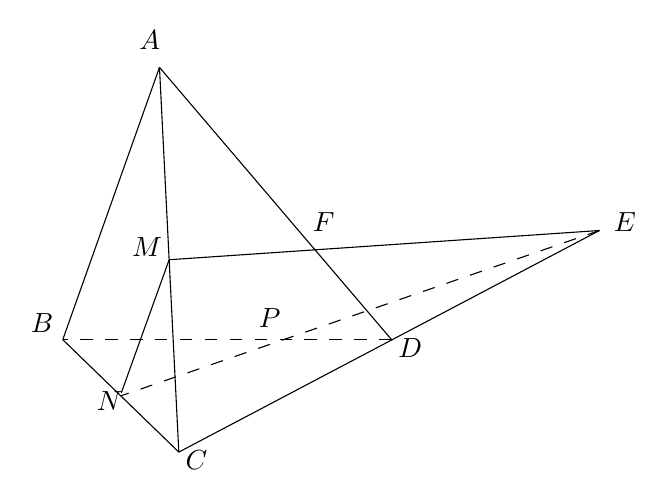
\begin{tikzpicture}[x=0.75pt,y=0.75pt,yscale=-1,xscale=1]
     \draw [dash pattern={on 4.5pt off  4.5pt}] (378.21,174.4) -- (219.79,174.4);
     \draw  (219.79,174.4) -- (275.7,228.57);
     \draw (266.38,43.21) -- (219.79,174.4); 
     \draw (266.38,43.21)  -- (275.7,228.57);
      \draw (266.38,43.21) -- (378.21,174.4);
     \draw (478.38,121.8) --  (275.7,228.57);
     \draw (271.04,135.89)  -- (248,200);
     \draw [dash pattern={on 4.5pt off 4.5pt}] (478.38,121.8) -- (247.75,201.49); 
     \draw (271.04,135.89) --  (478.38,121.8);
     \draw (255.4,24.35)  node [anchor=north west][inner sep=0.75pt] [align=left] {$A$};
     \draw  (203.15,160.56) node [anchor=north west][inner sep=0.75pt] [align=left] {$B$};
     \draw (277.7,226.79) node [anchor=north  west][inner sep=0.75pt] [align=left] {$C$};
      \draw (380.21,172.61) node [anchor=north west][inner sep=0.75pt] [align=left] {$D$};
      \draw (484,112) node [anchor=north west][inner sep=0.75pt] [align=left] {$E$};
     \draw  (252,124) node [anchor=north west][inner sep=0.75pt] [align=left] {$M$};
     \draw (235,198) node [anchor=north west][inner sep=0.75pt] [align=left]  {$N$};
     \draw (313,158) node [anchor=north  west][inner sep=0.75pt] [align=left] {$P$};
     \draw (339,112) node [anchor=north  west][inner sep=0.75pt] [align=left] {$F$};
    \end{tikzpicture}
  \end{center}
  \begin{itemchoice}
   \itemch Đúng. $NM$  là giao tuyến của hai mặt phẳng $\left(MNP\right)$,$ (ABC)$.
   \itemch Đúng. $DC$ là giao tuyến của hai mặt phẳng  $\left(BCD\right),(ADC)$.
    \itemch Đúng. Tìm giao điểm của $ CD$ và mặt phẳng $ (MNP)$:\\
   Trong mặt phẳng $ (BCD)$, vì $ NP$  và $ CD$ không song song nhau nên ta có thể gọi $ E=CD\cap NP$.\\
   Trong mặt phẳng $ (BCD)$, vì $ NP$ và  $ CD$ không song song nhau nên ta có thể gọi $ E=CD\cap NP$.\\
   Vì  $\heva{
   &{E\in CD}\\ 
    &{E\in NP,NP\subset (MNP).}
   }$ \\ 
   $\Rightarrow E=CD\cap  (MNP)$.
    \itemch Sai. Tìm giao điểm của $ AD$ và $ (MNP)$ :\\
   Xét mặt  phẳng phụ là $ (ACD)$ chứa $ AD$. Ta cần tìm giao tuyến của hai mặt phẳng $ (ACD)$ và $ (MNP)$.\\
   Vì $ M\in  AC,AC\subset (ACD)\Rightarrow M\in (ACD)\Rightarrow M\in (ACD)\cap (MNP).\quad(1)$\\
   Theo câu  a), ta có $\heva{
   &{E\in  CD,CD\subset (ACD)}\\
   &{E\in  (MNP).}
   }$  \\
   $\Rightarrow E\in (ACD)\cap  (MNP).\quad(2)$\\
   Từ $(1)$ và $(2)$ suy ra $ ME=(ACD)\cap (MNP)$.\\ 
   Trong mặt phẳng $ (ACD)$,  gọi $ F=AD\cap ME$.\\
    Vì $\heva{
   &{F\in AD}\\ 
   &{F\in  ME,ME\subset (MNP).}}$
  \end{itemchoice}
 } 
\end{ex}

% nguồn: Ok_dungsai_lop11_Lan1
\begin{ex}%[1H4H1-3]%[1H4H1-4]%[ma:997dca1d]
 Cho  hình bình hành $ABCD$ và một điểm $S$ không thuộc mặt phẳng $(ABCD)$, các điểm $M, N$ lần lượt là trung điểm của đoạn thẳng $AB, SC$. Gọi $O=AC\cap BD$.
  \choiceTF
  {\True $SO$ giao tuyến của hai mặt  phẳng $(SAC)$ và $(SBD)$}
  {\True Giao điểm của  $I$ của đường thẳng $AN$ và mặt phẳng $(SBD)$ là điểm nằm trên đường thẳng $SO$}
  {Giao điểm của $J$ của đường thẳng $MN$ và  mặt phẳng $(SBD)$ là điểm nằm trên đường thẳng $SD$}
  {\True  Ba điểm $I, J, B$ thẳng hàng}
 \loigiai{ 
  \begin{center}
   \begin{tikzpicture}[scale=0.8,font=\footnotesize,line join=round,line cap=round,>=stealth]
      \coordinate (A) at (0,0);
     \coordinate (B)  at (2,-2);
     \coordinate (D)  at (5,0);
     \coordinate (C) at ($(B)+(D)-(A)$); 
      \coordinate (S) at ($(A)+(50:6)$);
     \coordinate (N)  at ($(S)!0.5!(C)$);
      \coordinate (M) at ($(A)!0.5!(B)$);
     \coordinate (O) at (intersection of A--C and B--D); 
     \coordinate (I) at  (intersection of A--N and S--O);
     \coordinate (P) at  (intersection of C--M and B--D);
     \coordinate (J) at (intersection of S--P and M--N); 
     \draw  (S)--(A)
       (S)--(B)
      (S)--(C) 
       (A)--(B)--(C);
     \draw[dashed]  (S)--(D)
       (S)--(O)
      (A)--(D)--(C) 
       (A)--(C)
      (B)--(D) 
       (M)--(N)--(A)
      (S)--(P) 
       (C)--(M);
     \foreach \i/\g in {S/90,A/180,B/-90,C/-90,D/0,M/180,N/0,I/60,J/160,P/-90,O/0}{\draw[fill=black](\i) circle (.5pt) 
      ($(\i)+(\g:3mm)$)  node[scale=1]{$\i$};}
    \end{tikzpicture}
  \end{center}
  \begin{itemchoice}
    \itemch Đúng. $SO$ giao tuyến của hai mặt phẳng $(SAC)$ và $(SBD)$.
   \itemch  Đúng.
   Trong mặt  phẳng $(ABCD)$, gọi $O=AC\cap BD$.\\
   Trong mặt  phẳng $(SAC)$, gọi $I=SO\cap AN$.\\
    Ta có
   $\heva{ 
   & I\in AN\\ 
   & I\in SO,  SO\subset (SBD)
    }
    \Rightarrow I=AN\cap (SBD)$.
   \itemch Sai. Tìm giao điểm $J$ của $MN$ và mặt  phẳng $(SBD)$:\\
   Trong mặt  phẳng $(ABCD)$, gọi $P=CM\cap BD$;\\
   Trong mặt phẳng $(SCM)$, gọi  $J=MN\cap SP$;\\
    Ta có
   $\heva{ 
   & J\in MN\\ 
   & J\in SP, SP\subset (SBD) 
   } 
   \Rightarrow J=MN\cap  (SBD)$.
    \itemch Đúng. Dễ thấy $B\in (ABN)\cap (SBD) \quad (1)$.\\
   Ta có $\heva{ 
   &  I\in AN, AN\subset (ABN)\\
   & I\in SO,  SO\subset (SBD)
   } 
   \Rightarrow I\in (ABN)\cap (SBD) \quad (2)$.\\ 
    Tương tự:
    $\heva{
   & J\in MN, MN\subset (ABN)\\ 
    & \in SP, SP\subset (SBD)
   } 
    \Rightarrow J\in (ABN)\cap (SBD) \quad (3)$.\\
   Từ $(1)$, $(2)$, $(3)$ suy ra $B, I, J$ cùng thuộc giao tuyến của hai  mặt phẳng $(ABN)$ và $(SBD)$ nên ba điểm này thẳng hàng.
  \end{itemchoice}
  }
\end{ex}

% nguồn: Ok_dungsai_lop11_Lan1
\begin{ex}%[1H4H1-3]%[ma:8e7147a7]
 Cho hình chóp $ S.ABCD$, biết $ AB$ cắt $ CD$ tại $  E,AC$ cắt $ BD$ tại $ F$ trong mặt phẳng đáy. Khi đó:
  \choiceTF
  {\True Đường thẳng $ EF$ nằm trong  mặt phẳng $ (ABCD)$}
  {\True $ AB$ là  giao tuyến của hai mặt phẳng $ (SAB)$ và $ (ABCD)$}
  { $ SF$ là giao tuyến của hai mặt phẳng $ (SAB)$ và $ (SCD),$ $ SE$ là  giao tuyến của hai mặt phẳng $ (SAC)$ và $ (SBD)$}
  { Gọi $ G=EF\cap AD$ khi đó, $ SG$  giao tuyến của mặt phẳng $ (SEF)$ và mặt phẳng $ (SAD)$}
  \loigiai{
  \begin{itemchoice}
   \itemch Đúng.  Ta có $ E=AB\cap CD\Rightarrow E\in AB,AB\subset (ABCD)\Rightarrow E\in (ABCD)$.\\
   Tương  tự: $ F=AC\cap BD\Rightarrow F\in AC,AC\subset (ABCD)\Rightarrow F\in (ABCD)$. \\Vậy $ EF\subset (ABCD)$.
   \itemch Sai. Dễ thấy $ A$ là điểm chung của hai mặt phẳng $ (SAB)$ và $ (ABCD),B$  cũng là điểm chung của hai mặt phẳng $ (SAB)$ và $ (ABCD)$.\\
   Suy ra $ AB=(SAB)\cap  (ABCD)$.
   \begin{center}
    \tikzset{every picture/.style={line  width=0.75pt}}
    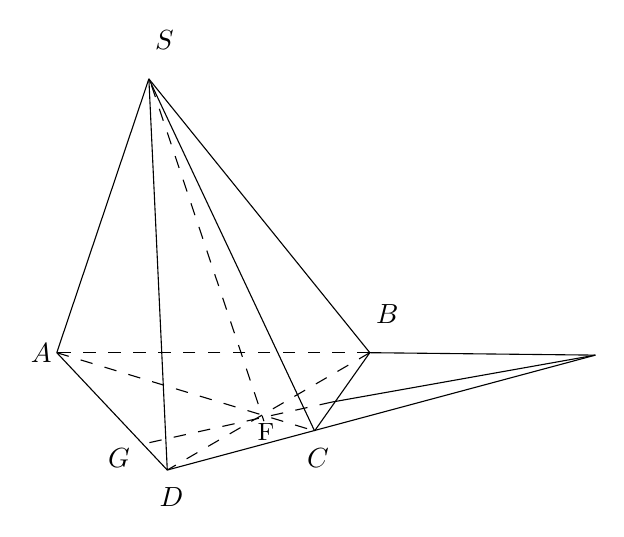
\begin{tikzpicture}[x=0.75pt,y=0.75pt,yscale=-1,xscale=1]
      \draw [dash pattern={on 4.5pt off  4.5pt}] (368.33,176.19) -- (217.52,176.19);
      \draw (217.52,176.19)  -- (270.75,232.73);
      \draw (477,177.37) -- (270.75,232.73); 
       \draw (368.33,176.19) -- (341.72,213.88);
      \draw (261.88,44.27) --  (217.52,176.19);
      \draw (261.88,44.27) -- (270.75,232.73); 
      \draw (261.88,44.27) --  (341.72,213.88);
      \draw (261.88,44.27) --  (368.33,176.19);
      \draw  [dash pattern={on 4.5pt off 4.5pt}] (217.52,176.19) -- (299.85,201.18) -- (341.72,213.88);
       \draw [dash pattern={on 4.5pt off 4.5pt}] (368.33,176.19) -- (270.75,232.73);
      \draw [dash pattern={on 4.5pt  off 4.5pt}] (263.12,47.34) -- (317.32,209.17);
       \draw (368.33,176.19) -- (477,177.37);
      \draw (477,177.37)  -- (350,200);
      \draw [dash pattern={on 4.5pt off 4.5pt}] (350,200) --  (260,220);
      \draw (263.64,19.87) node  [anchor=north west][inner sep=0.75pt] [align=left] {$S$};
      \draw (203.76,170.64) node [anchor=north west][inner sep=0.75pt] [align=left]  {$A$};
      \draw (370.09,151.79) node [anchor=north  west][inner sep=0.75pt] [align=left] {$B$};
      \draw (336.83,221.29) node [anchor=north west][inner sep=0.75pt]  [align=left] {$C$};
      \draw (265.86,240.13) node [anchor=north west][inner sep=0.75pt] [align=left] {$D$}; 
      \draw (313,209) node [anchor=north west][inner sep=0.75pt] [font=\small]  [align=left] {F};
      \draw (241,221) node [anchor=north west][inner sep=0.75pt] [align=left]  {$G$};
     \end{tikzpicture}
   \end{center}
   \itemch Đúng. Tìm giao tuyến của $ (SAB)$ và $ SCD)$  :\\
   Dễ thấy $ S$ là điểm chung của  hai mặt phẳng $ (SAB)$ và $ (SCD)$.\\
   Ta có  $\heva{
    &{E\in AB,AB\subset (SAB)}\\
   &{E\in CD,CD\subset  (SCD)}
   .}$\\ 
   Vậy $ SE=(SAB)\cap  (SCD)$.\\
   Tìm giao tuyến của $ (SAC)$ và $ (SBD)$  :\\
   Dễ thấy  $ S$ là điểm chung của hai mặt phẳng $ (SAC)$ và $ (SBD)$.\\
   Ta có  $\heva{
    &{F\in AC,AC\subset (SAC)}\\
   &{F\in BD,BD\subset  (SBD).}
    }$\\
    Vậy $ SF=(SAC)\cap (SBD)$.
   \itemch Đúng. Tìm giao tuyến của $ (SEF)$ với $ (SAD)$ :\\ 
   Dễ thấy $ S$ là điểm chung  của hai mặt phẳng $ (SEF)$ và $ (SAD)$.\\
   Trong mặt phẳng $ (ABCD)$, gọi $ G=EF\cap AD$.\\ 
   Ta có  $ \heva{
   {G\in EF,EF\subset (SEF)}\\ 
    {G\in AD,AD\subset (SAD)}.}$\\
   Vậy  $SG=(SEF)\cap (SAD)$.
  \end{itemchoice}
  }
\end{ex}

% nguồn: Ok_dungsai_lop11_Lan1
\begin{ex}%[1H4H1-3]%[ma:fd8f0ee3]
 Cho tứ diện $ABCD$. Gọi $I$, $J$  lần lượt là trung điểm của $AD$, $BC$, $M$ là một điểm trên cạnh
 $AB$, $N$ là  một điểm trên cạnh $AC$. Khi đó
  \choiceTF
   {\True $IJ$ là giao tuyến của hai mặt phẳng $(IBC)$ và $(JAD)$}
  {\True $ND$ là giao tuyến của hai mặt phẳng $(MND)$ và  $(ADC)$}
  {\True $BI$ là giao tuyến của hai mặt  phẳng $(BCI)$ và $(ABD)$}
  {Giao tuyến của hai mặt phẳng $(IBC)$ và $(DMN)$ song song  với đường thẳng $IJ$}
 \loigiai{ 
  \begin{center}
   \begin{tikzpicture}[scale=1,line join=round,font=\footnotesize,line cap=round,>=stealth,thick]
      \def\a{4.5}
     \path (0:0) coordinate  (B)
      ++(0:1.2*\a) coordinate  (D)
      ++(-150:\a) coordinate (C) 
      ($(B)+(70:\a)$) coordinate (A); 
      \path ($(A)!0.5!(D)$) coordinate (I);
      \path ($(B)!0.5!(C)$) coordinate (J);
     \path  ($(A)!0.3!(B)$) coordinate (M);
     \path ($(A)!0.4!(C)$) coordinate  (N);
     \coordinate (K) at (intersection  of B--I and M--D);
     \coordinate (L) at (intersection of  C--I and N--D);
     \draw[dashed,thick] (B)--(D) 
       (I)--(J)
       (M)--(D)
       (B)--(I)
      (J)--(D); 
     \draw[thick]  (B)--(A)--(D)
      (A)--(C) 
      (B)--(C)--(D) 
       (D)--(N)--(M)
       (I)--(C)
       (J)--(A);
      \foreach \x/\g in {A/90,B/180,C/-45,D/0,I/45,J/180,M/180,N/30,K/90,L/-90}
      \fill[black] (\x) circle (1pt)
      ($(\g:3mm)+(\x)$)  node {$\x$};
    \end{tikzpicture}
  \end{center}
  \begin{itemchoice}
   \itemch{\bf Đúng.}\\ 
   Ta có  $\heva{&I\in (IBC)\\&I\in AD\\&AD\subset (JAD)}\Rightarrow I\in (IBC)\cap (JAD).\quad (1)$\\
   Mặt khác  $\heva{&J\in (JAD)\\&J\in BC\\&BC\subset (IBC)}\Rightarrow J\in (IBC)\cap (JAD).\quad (2)$\\
   Từ $(1)$  và $(2)\Rightarrow IJ=(IBC)\cap (JAD)$.
   \itemch{\bf  Đúng.}\\
   Ta có $\heva{&ND\subset  (MND)\\&ND\subset (ADC)}\Rightarrow ND=(MND)\cap(ADC)$.
    \itemch{\bf Đúng.}\\
   Ta có $\heva{&BI\subset  (BCI)\\&BI\subset (ABD)}\Rightarrow BI=(BCI)\cap(ABD)$.
   \itemch{\bf Sai.}\\ 
   Gọi $K=BI\cap MD$ và $L=CI\cap ND\Rightarrow KL=(IBC)\cap (DMN)$.\\ 
   Mà $KL$ không song song $IJ$.\\ 
   Do đó giao tuyến  của hai mặt phẳng $(IBC)$ và $(DMN)$ không song song với đường thẳng $IJ$.
  \end{itemchoice}
  }
\end{ex}

% nguồn: Ok_dungsai_lop11_Lan1
\begin{ex}%[1H4H1-3]%[ma:d5d08029]
 Cho tứ giác $ ABCD$ có $ AC$ và $ BD$ giao nhau tại $ O$ và một điểm $ S$ không thuộc mặt phẳng $ (ABCD)$. Trên đoạn $ SC$ lấy một điểm $ M$ không trùng với $ S$ và $ C$,$ K=AM\cap SO$. Khi  đó:
  \choiceTF
  {$ SO$  là giao tuyến của hai mặt phẳng $\left(SAC\right)$,$ (ABC)$}
  {\True $ SO$ là giao tuyến của hai mặt  phẳng $\left(SAC\right)$,$ (SBD)$}
  {\True Giao điểm của đường thẳng $ SO$ với mặt phẳng $ (ABM)$ là điểm $ K$} 
  {Giao điểm của đường thẳng $ SD$ với mặt phẳng $ (ABM)$ là điểm $ N$ thuộc đường  thẳng $ AK$}
 \loigiai{ 
  \begin{itemchoice}
   \itemch  Sai. $ AC$ là giao tuyến của hai mặt phẳng $\left(SAC\right)$,$ (ABC)$.
   \itemch Đúng. $SO$ là giao tuyến của hai mặt phẳng $\left(SAC\right)$,$ (SBD)$. 
   \itemch Đúng. Tìm giao điểm của $ SO$  và $ (ABM)$ :\\
   Trong mặt phẳng $ (SAC)$, gọi $ K=AM\cap  SO$.\\
    $\heva{
   &{K\in  AM,AM\subset (ABM)}\\
   &{K\in  SO}}
    \Rightarrow K=SO\cap (ABM).$\\
   \begin{center}
    \tikzset{every picture/.style={line  width=0.75pt}}
    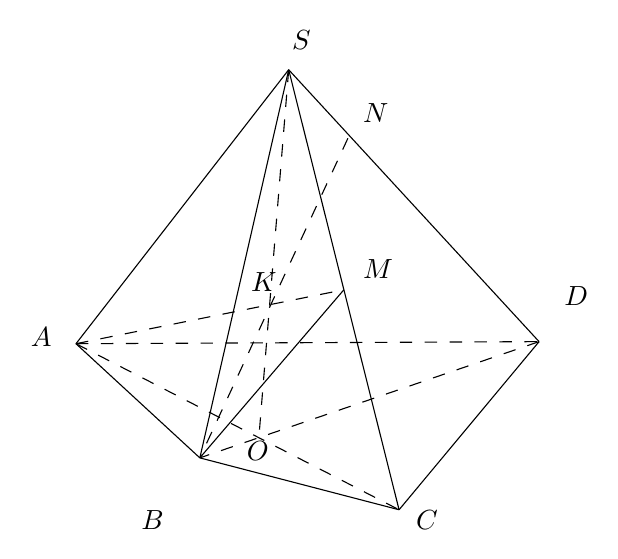
\begin{tikzpicture}[x=0.75pt,y=0.75pt,yscale=-1,xscale=1]
      \draw [color={rgb,255:red,0; green,0; blue,0},draw  opacity=1] [dash pattern={on 4.5pt off 4.5pt}] (157.94,176) -- (381.06,175);
      \draw [color={rgb,255:red,0; green,0; blue,0},draw  opacity=1] (157.94,176) -- (217.61,231);
      \draw [color={rgb,255:red,0; green,0; blue,0},draw opacity=1] (381.06,175) --  (313.6,256);
       \draw [color={rgb,255:red,0; green,0; blue,0},draw opacity=1] (217.61,231) -- (313.6,256);
      \draw [color={rgb,255:red,0;  green,0; blue,0},draw opacity=1] (260.42,44) -- (157.94,176);
      \draw [color={rgb,255:red,0; green,0;  blue,0},draw opacity=1] (260.42,44) -- (217.61,231);
      \draw [color={rgb,255:red,0; green,0; blue,0},draw opacity=1] (260.42,44) -- (313.6,256); 
      \draw [color={rgb,255:red,0; green,0; blue,0},draw opacity=1] (260.42,44)  -- (381.06,175);
      \draw [dash pattern={on 4.5pt off 4.5pt}] (381.06,175) -- (217.61,231); 
      \draw [dash pattern={on  4.5pt off 4.5pt}] (157.94,176) -- (313.6,256);
      \draw [dash pattern={on 4.5pt off 4.5pt}] (260.42,44) --  (246.15,220);
      \draw [dash  pattern={on 4.5pt off 4.5pt}] (157.94,176) -- (287.01,150);
      \draw [dash pattern={on 4.5pt off 4.5pt}]  (288.96,77) -- (217.61,231);
      \draw (287.01,150)  -- (217.61,231);
      \draw (260.76,24) node [anchor=north west][inner sep=0.75pt] [align=left] {$S$}; 
      \draw (134.93,167) node [anchor=north  west][inner sep=0.75pt] [align=left] {$A$};
      \draw  (391.92,147) node [anchor=north west][inner sep=0.75pt] [align=left] {$D$};
      \draw (188.12,255) node [anchor=north west][inner sep=0.75pt] [align=left] {$B$}; 
      \draw (320.58,255) node [anchor=north west][inner  sep=0.75pt] [align=left] {$C$};
      \draw (295,59) node [anchor=north west][inner sep=0.75pt] [align=left]  {$N$};
      \draw  (295,134) node [anchor=north west][inner sep=0.75pt] [align=left] {$M$};
      \draw (241.02,140.5) node [anchor=north west][inner sep=0.75pt]  [align=left] {$K$};
      \draw (239,222) node [anchor=north west][inner sep=0.75pt] [align=left] {$O$}; 
     \end{tikzpicture}
   \end{center}
   \itemch Sai. Tìm giao điểm của $SD$ và $ (ABM)$:\\ 
   Xét mặt  phẳng phụ $ (SBD)$ chứa $SD$.\\
   Dễ thấy $B$ là điểm  chung của hai mặt phẳng $(SBD)$ và $ (ABM)$.\\
   Ta  có $\heva{
   &{K\in AM,AM\subset (ABM)}\\ 
   &{K\in SO,SO\subset (SBD).} 
   }$ \\ 
   $\Rightarrow K\in  (SBD)\cap (ABM)$.\\
   Do  đó $ BK=(SBD)\cap (ABM)$.\\
   Trong mặt phẳng  $ (SBD)$, gọi $ N=BK\cap SD$.\\
    Vì $\heva{
   &{N\in SD}\\ 
   &{N\in  BK,BK\subset (ABM)}
   }\Rightarrow  N=SD\cap (ABM).$\\
  \end{itemchoice}
  }
\end{ex}

% nguồn: Ok_dungsai_lop11_Lan1
\begin{ex}%[1H4H1-3]%[ma:c714339b]
 Cho tứ diện $ABCD$ với $I$  và $J$ lần lượt là trung điểm các cạnh $AB$ và $CD$.
 \choiceTF 
  {\True $IJ$ là giao tuyến của mặt phẳng  $(ABJ)$ và $(CID)$}
  {\True$CD$ là giao tuyến của mặt phẳng $(ACD)$  và $(BCD)$ }
  {Bốn điểm $I$, $J$, $B$, $D$ đồng  phẳng}
  {\True Bốn điểm $I$, $J$, $C$, $D$  đồng phẳng}
 \loigiai{\immini{ 
  \begin{itemchoice}
   \itemch Ta  có\\
   $\heva{&I\in (ICD)\\&I\in AB \subset (ABJ)}\Rightarrow  I\in (ABJ)\cap (ICD)$.\\
   $\heva{&J\in (ABJ)\\&J\in CD\subset (ICD)}\Rightarrow J\in  (ABJ)\cap (ICD)$.\\
    Từ đó suy ra $IJ=(ABJ)\cap (ICD)$.
   \itemch $(ACD)\cap (BCD)=CD$. 
   \itemch Vì $J\in (BCD)$ và  $I\notin (BCD)$ nên bốn điểm $I$, $J$, $B$, $D$ không đồng phẳng.
   \itemch Ta  có $J \in CD \subset (CID) \Rightarrow J \in (CID)$.\\
   Vậy bốn điểm $I$, $J$,  $C$, $D$ đồng phẳng.
  \end{itemchoice}
   }
  {\begin{tikzpicture}[scale=.5,font=\footnotesize,line join=round,line cap=round,>=stealth]
   \path
   (-1,0)  coordinate (B)
    (2,-2) coordinate (C)
   (6,0) coordinate  (D)
    ($(B)+(2,6)$) coordinate (A)
    ($(A)!1/2!(B)$) coordinate (I)
   ($(C)!1/2!(D)$) coordinate  (J);
  \draw[dashed] (D)--(B) 
    (D)--(I)
   (I)--(J); 
  \draw  (C)--(I)
    (C)--(A)
    (A)--(B)--(C)--(D)--cycle;
  \foreach \p/\g in {A/90,C/-90,B/180,D/0,J/-45,I/135} 
   \draw[fill=black] (\p) circle (.5pt) +(\g:.3) node{$\p$};
 \end{tikzpicture}
  } 
 } 
\end{ex}

% nguồn: Ok_dungsai_lop11_Lan1
\begin{ex}%[1H4H1-3]%[ma:7c019b6d]
 Cho tứ diện $ABCD$. Gọi $M$ là điểm trên cạnh $AB, N$ là điểm thuộc cạnh $AC$ sao cho $MN$ không song  song với $BC$. Gọi $P$ là điểm nằm trong $\triangle BCD$. Khi đó:
  \choiceTF
  {\True  $MN=(MNP)\cap (ABC)$}
  {\True Giao tuyến của hai mặt phẳng $(MNP), (BCD)$ là đường  thẳng cắt $BC$}
  {Giao tuyến  của hai mặt phẳng $(MNP), (ABD)$ là đường thẳng cắt $AB$ và $DC$}
  {Giao tuyến của hai mặt phẳng  $(MNP), (ACD)$ là đường thẳng cắt $AB$ và $DC$}
  \loigiai{
  \begin{itemchoice}
   \itemch Đúng. $MN=(MNP)\cap  (ABC)$.
   \itemch Đúng. Trong $(ABC)$  gọi $H=MN \cap BC$.\\
    Ta có
    $\heva{
   & H\in MN\subset (MNP)\\ 
   &  H\in BC\subset (BCD)
   } 
   \Rightarrow  H\in (MNP) \cap (BCD)\quad (1)$.\\
   Lại có: 
    $\heva{
   & P\in  (MNP)\\
   & P\in (BCD) 
   } 
   \Rightarrow P\in (MNP)\cap (BCD)  \quad (2)$.\\
   Từ $(1)$  và $(2)$ suy ra $HP=(MNP)\cap (BCD)$.\\
   \begin{center}
    \begin{tikzpicture}[scale=1,font=\footnotesize,line join=round,line cap=round,>=stealth]
      \path 
      (-2,0)  coordinate (B)
      (1,-2) coordinate (D) 
      (3,0) coordinate  (C)
       ($(B)+(2,3)$) coordinate (A)
      (0.5,-0.5)  coordinate (P)
      ($(A)!0.4!(B)$) coordinate  (M)
      ($(A)!0.6!(C)$) coordinate (N) 
      ($(M)!2!(N)$) coordinate (x) 
      ($(B)!2!(C)$)  coordinate (y);
       \coordinate (H) at (intersection of M--x and B--y);
      \path  ($(H)!2!(P)$) coordinate (z);
      \coordinate (F) at (intersection of H--P  and C--D);
      \coordinate (K) at (intersection of H--z and  B--D);
      \draw (A)--(B) 
      (A)--(D) 
      (A)--(C) 
      (B)--(D)--(C) 
      (N)--(H)--(F) 
      (M)--(K) 
       (N)--(F);
       \draw [dashed] (N)--(B)--(C)--(H)
       (F)--(K)
      (M)--(P)--(N)--cycle; 
       \foreach \x/\g in {A/90,B/180,D/-90,C/50,M/150,N/50,P/-90,H/0,F/-90,K/-90} \draw[fill=black](\x) circle (.5pt)
      ($(\x)+(\g:3mm)$)  node[scale=1]{$\x$};
     \end{tikzpicture}
   \end{center}
   \itemch Sai. Trong $(BCD)$ gọi  $K=HP\cap BD$.\\
    Ta có
    $\heva{
    & K\in BD \subset (ABD)\\
   & K\in HP \subset  (MNP)
    }
   \Rightarrow K\in (MNP) \cap  (ABD) \quad (1)$.\\
    Lại có
   $\heva{ 
    & M\in (MNP)\\
   & M\in AB  \subset (ABD)
   } 
   \Rightarrow M\in (MNP)\cap  (ABD) \quad (2)$.\\
   Từ $(1)$ và $(2)$ suy ra $MK\in (MNP) \cap  (ABD)$.
   \itemch Sai. Trong  $(BCD)$ gọi $F=HK\cap DC$.\\
   Trình bày tương tự như hai câu trên ta  được $NF=(MNP) \cap (ACD)$.
  \end{itemchoice}
 } 
\end{ex}

% nguồn: Ok_dungsai_lop11_Lan1
\begin{ex}%[1H4H1-3]%[ma:7d057437]
 Cho hình chóp $S.ABCD$ có $ABCD$ là hình thang với hai cạnh đáy là $AD$ và $BC$, đáy lớn là $AD$. Gọi $M$,  $N$ lần lượt là trung điểm của $SA$ và $SD$.
 \choiceTF 
  {\True  $MN$ song song $BC$}
  {\True Giao tuyến của $(SAD)$ và $(SBC)$ là đường  thẳng qua $S$ và song song với $AD$}
  {\True Giao điểm của $SB$ và $(MCD)$  là $F=SB\cap ME$}
  {Giao tuyến của $(SAB)$ và $(SCD)$  là đường thẳng qua $S$ và song song với $AB$}
  \loigiai{
  \begin{center}
   \begin{tikzpicture}[scale=1,font=\footnotesize,line join=round,line cap=round,>=stealth]
     \path  (0,0) coordinate (B)
       (3,0) coordinate (C)
      (1,1)  coordinate (A)
      ($(A)+(C)-(B)+(1.5,0)$) coordinate (D) 
      (0.3,2.7) coordinate  (h)
      ($(A)+(h)$) coordinate (S) 
      ($(S)!0.5!(A)$) coordinate (M) 
      ($(S)!0.5!(D)$)  coordinate (N)
      (intersection of A--B and C--D)  coordinate (E)
      (intersection of S--B and M--E) coordinate  (F);
      \draw (S)--(F)--(C)--(D)--cycle (S)--(C)--(F)--(E)--(C);
     \draw[shorten <=-1cm,shorten >=-1cm] (S)--+(2.5,0)  node[pos=1.2,above]{$x$};
      \draw[dashed] (S)--(A)--(B)--(F)--(M)--(D)--(A)
       (E)--(B)--(C)--(M)--(N);
     \foreach \p/\g in {A/150,B/-60,C/-60,D/0,S/90,M/45,N/30,E/-90,F/150} \fill[black]  (\p) circle (1pt)+(\g:0.3) node{$\p$};
    \end{tikzpicture}
  \end{center}
  \begin{itemchoice}
   \itemch{\bf Đúng.}\\ 
    Ta có $MN$ là đường trung bình của tam giác $SAD$ nên $MN\parallel AD$.\\
   Vì $ABCD$ là hình thang  nên $BC\parallel AD$.\\
   Suy  ra $MN\parallel BC$.
   \itemch{\bf  Đúng.}\\
   Ta có $\heva{&S\in (SAD)\cap (SBC)\\ & AD\parallel  BC \\ & AD\subset (SAD)\\ & BC\subset (SBC) }\Rightarrow (SAD)\cap (SBC)=Sx$, trong đó $Sx\parallel AD\parallel BC$
    \itemch{\bf Đúng.}\\
   Ta  có $SB\subset (SAB)$.\\
   Trong $(ABCD)$  gọi $E=AB\cap CD$.\\
   Khi đó $\heva{& E\in  AB, AB\subset (SAB) \\ & E\in CD, CD\subset (MCD)}\Rightarrow E\in (SAB)\cap (MCD)$.\\
    Dễ thấy $M\in (SAB)\cap (MCD)$.\\
   Do đó, $(SAB)\cap (MCD)=ME$.\\ 
   Trong $(SAB)$, gọi $F=SB\cap ME$.\\ 
   Vậy  $F=SB\cap (MCD)$.
   \itemch{\bf Sai.}\\ 
   Ta có $S\in (SAB)\cap  (SCD)$.\\
   $\heva{&E\in AB\\&AB\subset  (SAB)}\Rightarrow E\in (SAB)$.\\
    $\heva{&E\in CD\\&CD\subset (SCD)}\Rightarrow E\in (SCD)$.\\
   Suy  ra $E\in (SAB)\cap (SCD)$.\\
    Vậy $(SAB)\cap (SCD)=SE$.
  \end{itemchoice}
 } 
\end{ex}

% nguồn: Ok_dungsai_lop11_Lan2
\begin{ex}%[1H4H1-3]%[ma:29cf60d3]
	Cho hình chóp ${S.ABCD}$, biết $AB$ cắt $CD$ tại $E$, $AC$ cắt  $BD$ tại $F$ trong mặt phẳng đáy. Xét tính đúng sai của các khẳng định sau
	 \choiceTF
		{\True Đường thẳng $EF$ nằm trong mặt phẳng $(ABCD)$} 
		{\True $A B$ là  giao tuyến của hai mặt phẳng $\left( SAB \right)$ và $(ABCD)$}
		{$SF$ là giao tuyến của hai mặt phẳng $\left( SAB \right)$ và $\left( SCD \right)$, $SE$ là giao tuyến của hai mặt phẳng $\left(  SAC \right)$ và ${(S B D)}$}
		{\True Gọi $G=E F  \cap A D$ khi đó, $SG$ giao tuyến của mặt phẳng $(S E F)$ và mặt phẳng $(S A D)$}
	\loigiai{ 
		\begin{center}
			\begin{tikzpicture}[scale=1.4,font=\small,line join=round,line cap=round,>=stealth]
					 \path
						(0,0) coordinate (A) 
						($(A)+(1.1,-2)$) coordinate (B) 
						($(B)+(2,0.9)$) coordinate (C) 
						 ($(A)+(4,0)$) coordinate (D)
						 ($(A)+(2,2)$) coordinate (S)
						(intersection of  A--C and B--D) coordinate (F)
						 (intersection of A--B and C--D) coordinate (E)
						(intersection of E--F and A--D) coordinate (G) 
						(intersection of E--F and  B--C) coordinate (a);
					\draw  (A)--(B)
						 (C)--(D)--(S)--(A)
						 (B)--(S)--(C)
						 (D)--(E)--(C)
						 (B)--(E)
						(S)--(E); 
					\draw [dashed]  (D)--(A)--(C)--(B)
						 (B)--(D)
						(a)--(G) 
						(S)--(F) 
						(S)--(G) 
						 (a)--(E);
					\foreach \x/\g in {A/180,B/180,C/-30,D/50,S/90,F/-90,G/20,E/-60} 
					\fill[black] (\x) circle  (1pt)
						($(\g:2mm)+(\x)$) node {$\x$}; 
				\end{tikzpicture}
		\end{center}
		\begin{itemchoice}
			\itemch Ta có $E\in AB\subset (ABCD)$. Tương tự $F\in (ABCD)$. Vậy $EF\subset (ABCD)$. 
			\itemch Dễ thấy $A$ là điểm chung của  hai mặt phẳng $\left( SAB \right)$ và $(ABCD)$, $B$ cũng là điểm chung của hai mặt phẳng $\left( SAB \right)$ và ${(ABCD)}$. Suy ra $AB=\left( SAB \right)\cap \left( ABCD \right)$.
			\itemch Tìm giao tuyến của $\left(  SAB \right)$ và $\left( SCD \right)$.
			Dễ thấy ${S}$ là điểm chung của hai mặt phẳng $\left( SAB \right)$  và $\left( SCD \right)$.
			Ta có $\heva{&E\in AB\subset(SAB)\\&E\in CD\subset(SCD)}\Rightarrow E\in \left( SAB  \right)\cap \left( SCD \right)$.\\
			Vậy $SE=\left( SAB  \right)\cap \left( SCD \right)$.\\
			 Tìm giao tuyến của $\left( SAC \right)$ và ${(S B D)}$.
			Dễ thấy ${S}$  là điểm chung của hai mặt phẳng ${(S A C)}$ và ${(S B D)}$.
			Ta có $\heva{&F\in AC\subset(SAC)\\&F\in BD\subset(SBD)}\Rightarrow F\in \left( SAC  \right)\cap \left( SBD \right) $.\\
			 Vậy $SF=\left( SAC \right)\cap \left( SBD \right)$.
			\itemch Tìm giao  tuyến của ${(S E F)}$ với ${(S A D)}$.
			Dễ thấy ${S}$ là điểm  chung của hai mặt phẳng ${(S E F)}$ và ${(S A D)}$.
			Trong mặt phẳng $\left( ABCD \right)$, gọi ${G=E F \cap  A D}$.\\
			Ta có: $\heva{&G\in EF\subset(SEF)\\&G\in AD\subset(SAD)}\Rightarrow G\in  \left( SEF \right)\cap \left( SAD \right)$.\\
			Vậy ${S G=(S E  F) \cap(S A D)}$.
		\end{itemchoice}
	 }
\end{ex}

% nguồn: Ok_dungsai_lop11_Lan2
\begin{ex}%[1H4H1-3]%[ma:a21675db]
	Cho tứ diện $A B C D$. Gọi $M$ là điểm trên cạnh $A B$, $N$ là điểm thuộc cạnh $AC$ sao cho $MN$ không song song với $BC$.  Gọi $P$ là điểm nằm trong $\triangle BCD$. Xét tính đúng sai của các khẳng định sau
	\choiceTF 
		{\True $MN=\left( MNP  \right)\cap \left( ABC \right)$}
		{\True Giao  tuyến của hai mặt phẳng $\left( MNP \right)$, $\left( BCD \right)$ là đường thẳng cắt $BC$}
		{Giao tuyến của hai mặt phẳng $\left( MNP \right)$, $\left( ABD \right)$ là đường thẳng  cắt $AB$ và $DC$}
		{Giao tuyến của hai mặt phẳng $\left(  MNP \right)$, $\left( ACD \right)$ là đường thẳng cắt $AB$ và $DC$}
	 \loigiai{
		\begin{center}
			\begin{tikzpicture}[scale=1.7,font=\small,line join=round,line cap=round,>=stealth]
					\path 
						(0,0) coordinate (B) 
						($(B)+(1,-1.5)$) coordinate (D) 
						 ($(B)+(3,0)$) coordinate (C)
						($(B)+(1,2)$) coordinate (A) 
						($(A)!0.3!(B)$)  coordinate (M)
						 ($(B)!0.45!(D)$) coordinate (K)
						 ($(A)!0.6!(C)$) coordinate (N)
						 (intersection of M--N and B--C) coordinate (H)
						(intersection of K--H and D--C)  coordinate (F)
						($(K)!0.4!(F)$) coordinate  (P);
					 \draw (A)--(B)--(D)--(F)
						 (N)--(A)--(D)
						(K)--(M) 
						 (N)--(F)--(H)--(N);
					\draw  [dashed] (M)--(N)--(P)--(M)
						(K)--(F) 
						 (B)--(H)
						(F)--(C)--(N); 
					 \foreach \x/\g in {A/90,B/180,D/-90,C/45,H/0,F/-45,P/-50,K/-135,N/45,M/135}
					\fill[black] (\x)  circle (1pt)
						($(\g:2mm)+(\x)$) node  {$\x$};
				\end{tikzpicture}
		\end{center}
		\begin{itemchoice}
			\itemch $MN=\left( MNP  \right)\cap \left( ABC \right)$.
			\itemch  Trong ${(A B C)}$ gọi ${H=M N \cap B C}$.\\
			Ta có $\heva{&H\in MB\subset(MNP)\\&H\in BC\subset(BCD)}\Rightarrow  H\in \left( MNP \right)\cap \left( BCD \right) \left( 1 \right)$.\\
			Lại có $\heva{&P\in (MPN)\\&P\in(BCD)}\Rightarrow P\in \left( MNP \right)\cap \left( BCD \right)\left( 2  \right)$.\\
			Từ $\left( 1 \right)$ và $\left( 2 \right)$  suy ra ${H P=(M N P) \cap(B C D)}$.
			\itemch Trong $(BCD)$  gọi $K=HP\cap BD$.\\
			Ta có $\heva{&K\in BD\subset(ABD)\\&K\in HP\subset(MNP)}\Rightarrow K\in \left( MNP \right)\cap  \left( ABD \right)\left( 1 \right)$.\\
			 Lại có $\heva{&M\in(MNP)\\&M\in AB\subset(ABD)}\Rightarrow M\in \left( MNP \right)\cap \left( ABD \right)\left( 2 \right)$.\\
			 Từ $\left( 1 \right)$ và $\left( 2 \right)$ suy ra $MK\in \left( MNP \right)\cap \left( ABD \right)$.
			\itemch  Trong ${(B C D)}$ gọi ${F=H K \cap D C}$.\\
			Trình bày tương tự như hai câu trên ta được $NF=(M  N P) \cap(A C D)$.
		\end{itemchoice}
	 }
\end{ex}

% nguồn: Ok_dungsai_lop11_Lan2
\begin{ex}%[1H4H1-3]%[ma:16eba254]
	Cho hình chóp $S.ABCD$ có đáy là hình thang $ABCD\left( AB\parallel CD \right).$ Xét tính đúng sai của các khẳng định  sau
	\begin{center}
		\begin{tikzpicture}[scale=1.4,font=\small,line join=round,line cap=round,>=stealth]
				 \path
					(0,0) coordinate  (A)
					($(A)+(0.5,-1.5)$) coordinate (D) 
					($(D)+(2,0)$) coordinate  (C)
					($(A)+(4,0)$) coordinate (B) 
					($(A)+(2,2)$)  coordinate (S)
					(intersection of A--C and B--D)  coordinate (O)
					(intersection of A--D and C--B) coordinate (I); 
				 \draw (B)--(C)
					 (D)--(S)--(A)--(D)
					(B)--(S)--(C) 
					(D)--(I)--(C) 
					 (S)--(I);
				\draw [dashed]  (A)--(B)--(D)
					 (A)--(C)
					(S)--(O) 
					(D)--(C); 
				 \foreach \x/\g in {A/180,B/0,C/0,D/180,S/90,O/-90,I/-90}
				\fill[black] (\x) circle  (1pt)
					($(\g:3mm)+(\x)$) node  {$\x$};
			\end{tikzpicture}
	\end{center}
	\choiceTF 
		{\True Hình chóp $S.ABCD$ có 4 mặt bên} 
		{\True Giao tuyến của hai mặt phẳng $\left( SAC \right)$ và $\left( SBD \right)$ là $SO$ $(O$  là giao điểm của $AC$ và $BD)$}
		{\True  Giao tuyến của hai mặt phẳng $\left( SAD \right)$ và $\left( SBC \right)$ là $SI$ $(I$ là giao điểm của $AD$ và $BC)$}
		{Giao tuyến của  hai mặt phẳng $\left( SAB \right)$ và $\left( SAD \right)$ là đường trung bình của $ABCD$}
	\loigiai{ 
		\begin{itemchoice}
			\itemch  Hình chóp $S.ABCD$ có 4 mặt bên: $\left( SAB \right),\ \left( SBC \right),\ \left( SCD \right),\ \left( SAD \right)$.
			\itemch $S$ là điểm chung thứ nhất của hai mặt phẳng $\left( SAC \right)$ và $\left( SBD \right)$.\\ 
			$\heva{&O\in AC\subset(SAC)\Rightarrow O\in (SAC)\\&O\in BD\subset(SBD)\Rightarrow O\in (SBD)}\Rightarrow O$ là điểm chung thứ hai của hai mặt phẳng $\left( SAC \right)$ và $\left( SBD \right)$ $\Rightarrow\left( SAC \right)\cap \left( SBD  \right)=SO$.
			\itemch Tương tự, ta có $\left( SAD \right)\cap \left(  SBC \right)=SI$.
			\itemch $\left( SAB \right)\cap \left( SAD \right)=SA$ mà  $SA$ không phải là đường trung bình của hình thang $ABCD$.
		\end{itemchoice}
	} 
\end{ex}

% nguồn: Ok_dungsai_lop11_Lan2
\begin{ex}%[1H4H1-3]%[ma:68651a09]
	Cho hình chóp $S.ABCD$ có đáy $ABCD$  là hình bình hành. Khi đó
	 \choiceTF
		{\True Giao tuyến của $(SAB)$ và $(SCD)$ là đường thẳng đi  qua $S$ và song song với $AB$}
		{Giao  tuyến $(SCD);(SAD)$ và $(SBC)$ là đường thẳng đi qua $S$ và song song với $AB$}
		{\True  Gọi $M\in SC$ giao tuyến của $(ABM)$ và $(SCD)$ là đường thẳng đi qua $M$ và song song với $AB$}
		{\True Gọi $N\in SB$ giao tuyến của $(SAB)$ và $(NCD)$ là đường thẳng đi qua $N$  và song song với $AB$}
	\loigiai{ 
		\begin{center}
			\begin{tikzpicture}[font=\footnotesize]
					 \def\a{4}
					\path 
						(0:0) coordinate  (A)
						 (0:4) coordinate (B)
						 ++(220:2.5) coordinate (C)
						($(A)+(C)-(B)$) coordinate  (D)
						($(A)+(75:3.5)$) coordinate (S) 
						($(S)+(B)-(A)$)  coordinate (Sx)
						 ($(S)+(D)-(A)$) coordinate (Sy)
						 ($(S)!.5!(C)$) coordinate (M)
						($(M)+(A)-(B)$) coordinate (Mt) 
						($(S)!.35!(B)$) coordinate (N) 
						($(N)+(A)-(B)$)  coordinate (Nz)
						(intersection  of N--Nz and S--D) coordinate (nz);
					\draw[dashed] (B)--(A)--(D) 
						(A)--(S) 
						(M)--(D)--(N) 
						(N)--(nz); 
					 \draw[] (S)--(B)--(C)--(D)--(S)--(C)
						 (C)--(N)
						 (B)--(M)
						 ($(S)!-2cm!(Sx)$) --(S)--(Sx) node[above]{$x$}
						 ($(S)!-2cm!(Sy)$) node[left]{$y$}--(S)--(Sy)
						 ($(M)!-2.75cm!(Mt)$) node[above]{$t$}--(M)--(Mt)
						 ($(N)!-2.5cm!(Nz)$) node[above]{$z$}--(N)
						(nz)--(Nz); 
					 \foreach \x/\y in {A/150,B/0,C/-90,D/-90,S/90,M/60,N/60}
					\fill[black]  (\x) circle (1pt)
						($(\y:3mm)+(\x)$) node {$\x$}; 
				\end{tikzpicture}
		\end{center}
		\begin{itemchoice}
			\itemch  Đúng.\\
			Ta  có $\heva{
			&AB\parallel CD  \\
			&AB\subset (SAB)  \\
			&CD\subset (SCD) \\ 
			&S\in (SAB)\cap (SCD) }$ $\Rightarrow 
			\heva{ 
			 &Sx=(SAB)\cap (SCD) \\
			&Sx\parallel AB\parallel CD. }$ 
			\itemch Sai.\\ 
			 Ta có $\heva{
			&AD\parallel  BC \\
			&AD\subset (SAD) \\ 
			&BC\subset (SBC)  \\
			&S\in (SAD)\cap (SBC) }$ $\Rightarrow 
			 \heva{
			&Sy=(SAD)\cap (SCD) \\ 
			&Sy\parallel AD\parallel BC. }$ 
			\itemch  Đúng.\\
			Ta có:  $\heva{
			&AB\parallel  CD \\
			&AB\subset  (MAB) \\
			&CD\subset (SCD) \\ 
			&M\in  (MAB)\cap (SCD) }$ $\Rightarrow
			\heva{ 
			&Mt=(MAB)\cap (SCD)  \\
			&Mt\parallel  AB\parallel CD.}$.
			\itemch Đúng.\\ 
			Ta  có $\heva{
			 &AB\parallel CD\\
			 &AB\subset (SAB)\\
			&CD\subset  (NCD)\\
			&N\in  (SAB)\cap (NCD)}$ $\Rightarrow
			\heva{ 
			 &Nz=(SAB)\cap (NCD)\\
			 &Nz\parallel AB\parallel CD.}$
		\end{itemchoice}
	} 
\end{ex}

% nguồn: Ok_dungsai_lop11_Lan2
\begin{ex}%[1H4H1-3]%[ma:fe7d9306]
	Cho tứ diện $ABCD$. Gọi $I$, $J$ lần  lượt là trung điểm của $AD$, $BC$, $M$ là một điểm trên cạnh $AB$, $N$ là một điểm trên cạnh $AC$. Khi đó:
	\choiceTF 
		{\True $IJ$ là giao tuyến của hai mặt phẳng $\left( IBC \right)$, $\left(  JAD \right)$}
		{\True $ND$ là giao tuyến của  hai mặt phẳng $\left( MND \right)$, $\left( ADC \right)$}
		{\True $BI$ là giao tuyến của hai  mặt phẳng $\left( BCI \right)$, $\left( ABD \right)$}
		{Giao tuyến của hai mặt phẳng $\left( IBC \right)$, $\left( DMN  \right)$ song song với đường thẳng $IJ$}
	\loigiai{ 
		\begin{center}
			\begin{tikzpicture}[scale=1.7,font=\small,line join=round,line cap=round,>=stealth]
					\path 
						(0,0) coordinate (B) 
						($(B)+(1,-1.5)$)  coordinate (C)
						 ($(B)+(3,0)$) coordinate (D)
						 ($(B)+(1,2)$) coordinate (A)
						($(A)!0.5!(D)$)  coordinate (I)
						($(B)!0.5!(C)$) coordinate (J) 
						($(A)!0.4!(B)$)  coordinate (M)
						 ($(A)!0.55!(C)$) coordinate (N)
						(intersection of M--D and B--I) coordinate  (F)
						 (intersection of C--I and D--N) coordinate (E);
					\draw (A)--(B)--(C)--(D)--(A)--(C) 
						 (M)--(N)--(D)
						(A)--(J) 
						 (C)--(I);
					 \draw [dashed] (B)--(I)
						(B)--(D) 
						(M)--(D)--(J)--(I) 
						 (F)--(E);
					\foreach \x/\g in  {A/90,I/45,D/0,C/-90,J/-135,B/180,M/135,N/-155,E/-60,F/90}
					 \fill[black] (\x) circle (1pt)
						 ($(\g:2mm)+(\x)$) node {$\x$};
				\end{tikzpicture}
		\end{center}
		\begin{itemchoice}
			\itemch Ta có: $I \in A D\subset(J A D) \Rightarrow I \in(J A D) \Rightarrow  I J \subset(J A D)$;\\
			$J \in B C \subset(I B  C) \Rightarrow J \in(I B C) \Rightarrow I J \subset(I B C)$.\\
			Vậy ${(I B C)  \cap(J A D)=I J}$.
			\itemch $ND$ là  giao tuyến của hai mặt phẳng $\left( MND \right)$, $\left( ADC \right)$.
			\itemch $BI$ là giao tuyến của  hai mặt phẳng $\left( BCI \right)$, $\left( ABD \right)$.
			 \itemch Gọi $E=DN\cap CI$ (trong $\left( ACD \right)$) và $F=DM\cap BI$ (trong $\left( ABD \right)$).\\
			Ta  có $\heva{&E\in DN\subset(DMN)\\&E\in IC\subset (IBC)}\Rightarrow E\in (DMN)\cap(IBC) (1)$.\\
			Tương tự $\heva{&F\in DM\subset(DMN)\\&F\in BI\subset(IBC)}\Rightarrow F\in (DMN)\cap(IBC) (2)$.\\ 
			Từ $\left( 1 \right)$ và $\left( 2 \right)$ suy ra ${(D M N)  \cap(I B C)=E F}$. Khi đó $EF$ cắt $IJ$.
		\end{itemchoice}
	} 
\end{ex}

% nguồn: Ok_dungsai_lop11_Lan1
\begin{ex}%[1H4V1-3]%[ma:80d30a42]
 Cho  tứ diện $ ABCD$. Gọi $ I,J$ lần lượt là trung điểm của $ AD,BC$, $ M$ là một điểm trên cạnh $ AB,N$ là một điểm trên cạnh $ AC$. Khi đó:
  \choiceTF
  {\True $IJ$ là giao tuyến của  hai mặt phẳng $ (IBC),(JAD)$}
  {\True  $ ND$ là giao tuyến của hai mặt phẳng $ (MND),(ADC)$}
  {\True $ BI$ là giao tuyến của hai mặt phẳng  $ (BCI),(ABD)$}
  { Giao  tuyến của hai mặt phẳng $ (IBC),(DMN)$ song song với đường thẳng $IJ$}
  \loigiai{
  \begin{center}
    \tikzset{every picture/.style={line width=0.75pt}}
   \begin{tikzpicture}[x=0.75pt,y=0.75pt,yscale=-1,xscale=1]
     \draw [dash pattern={on 4.5pt off  4.5pt}] (234.65,198.26) -- (460.31,197.32);
      \draw (234.65,198.26) -- (325.67,260.69);
     \draw  (460.31,197.32) -- (325.67,260.69);
     \draw (336.02,51.57) -- (460.31,197.32); 
     \draw (336.02,51.57) --  (325.67,260.69);
     \draw (336.02,51.57)  -- (234.65,198.26);
     \draw  (336.02,51.57) -- (280.16,229.48);
     \draw [dash  pattern={on 4.5pt off 4.5pt}] (460.31,197.32) -- (280.16,229.48);
     \draw [dash pattern={on 4.5pt off 4.5pt}] (398.17,124.44)  -- (280.16,229.48);
     \draw (303.87,96.17)  -- (331.48,150.51);
     \draw [dash pattern={on 4.5pt off  4.5pt}] (303.87,96.17) -- (460.31,197.32);
     \draw (460.31,197.32) -- (331.48,150.51); 
     \draw (398.17,124.44)  -- (325.67,260.69);
     \draw [dash pattern={on 4.5pt  off 4.5pt}] (398.17,124.44) -- (234.65,198.26);
     \draw [dash  pattern={on 4.5pt off 4.5pt}] (366.93,136.24) -- (376.91,166.98);
     \draw (204.19,189.74) node [anchor=north west][inner sep=0.75pt]  {$B$};
     \draw  (474.06,179.61) node [anchor=north west][inner sep=0.75pt] {$D$};
     \draw (321.65,266.98) node [anchor=north west][inner sep=0.75pt] {$C$}; 
     \draw (330.49,30.21) node [anchor=north west][inner sep=0.75pt] {$A$}; 
     \draw (286.35,68.21) node  [anchor=north west][inner sep=0.75pt] [align=left] {$M$};
     \draw (311.62,138.6) node [anchor=north west][inner sep=0.75pt] [align=left] {$N$}; 
     \draw (364,117) node [anchor=north west][inner sep=0.75pt]  [align=left] {$F$};
      \draw (378.91,169.98) node [anchor=north west][inner sep=0.75pt] [align=left] {$E$};
     \draw (266,234)  node [anchor=north west][inner sep=0.75pt] [align=left] {$J$};
     \draw  (402,102) node [anchor=north west][inner sep=0.75pt] [align=left] {$I$};
    \end{tikzpicture}
  \end{center}
  \begin{itemchoice}
   \itemch Đúng. Ta có $  I\in AD,AD\subset (JAD)\Rightarrow I\in (JAD)\Rightarrow IJ\subset (JAD)$; $ J\in BC$,\\
   $BC\subset  (IBC)\Rightarrow J\in (IBC)\Rightarrow IJ\subset (IBC)$. Vậy $ (IBC)\cap (JAD)=IJ$.
   \itemch Đúng. $ ND$ là giao tuyến của hai mặt phẳng $  (MND),(ADC)$.
   \itemch Đúng. $ BI$ là giao tuyến của hai mặt phẳng $  (BCI),(ABD)$.
   \itemch Sai. Gọi $ E=DN\cap CI$ trong $ mp(ACD)$  và $ F=DM\cap BI$ trong $ mp(ABD)$.\\
   $\heva{ 
    &{E\in DN,DN\subset (DMN)}\\
   &{E\in  IC,IC\subset (IBC)}.
   }$\\ 
   $\Rightarrow E\in  (DMN)\cap (IBC).\,(1)$ \\
    Tương tự:
   $\heva{  &F\in DM,DM\subset (DMN)\\&F\in BI,BI\subset (IBC)
   .}$  \\
    $\Rightarrow F\in (DMN)\cap (IBC).$\\
   Từ $(1)$ và $(2)$ suy ra  $ (DMN)\cap (IBC)=EF$.\\
   Khi đó $EF$ cắt $IJ$. 
  \end{itemchoice}
 } 
\end{ex}

% nguồn: Ok_dungsai_lop11_Lan1
\begin{ex}%[1H4V1-3]%[ma:ba71ca1c]
 Cho chóp tứ giác $S.ABCD$. Gọi $M$ trung điểm của $SD$, $O$ là giao điểm của $AC$ và  $BD$.
  \choiceTF
  {\True $SK$ là giao tuyến của  $(SAD)$ và $(SBC)$ với $K$ là giao điểm của đường thẳng $AD$ và đường thẳng $BC$}
  {Điểm $M$ nằm trên giao tuyến  của hai mặt phẳng $(SAC)$ và $(ABM)$}
  {\True Nếu $ABCD$ là hình bình hành  thì $OM$ song song với $SB$}
  {\True Giao tuyến của hai mặt phẳng $(SAC)$ và $(ABM)$ là đường thẳng $AI$  với $I$ là giao điểm của đường thẳng $SO$ và đường thẳng $BM$}
 \loigiai{ 
  \begin{center}
   \begin{tikzpicture}[scale=1,font=\footnotesize,line join=round,line cap=round,>=stealth]
      \def\a{4}
      \path (0:0) coordinate (A)
       ++(0:\a) coordinate (D)
      ++(-130:\a/2)  coordinate (C)
      ++(-165:2*\a/3)  coordinate (B)
       ($(A)+(70:\a)$) coordinate (S)
      (intersection of A--C and B--D) coordinate  (O)
      ($(S)!0.5!(D)$)  coordinate (M)
      (intersection of S--O  and B--M) coordinate (I)
      (intersection of B--C and A--D) coordinate (K); 
     \draw[dashed]  (A)--(D)
      (B)--(M)--(A)--(C)--(D) 
       (B)--(D)--(K)
      (D)--(S)--(O); 
     \draw (A)--(B)--(C)--(K) 
      (A)--(S) 
      (B)--(S) 
       (C)--(S)
       (S)--(K);
      \foreach \x/\g in {A/180,B/-135,C/-45,D/45,S/90,O/-90,M/45,I/135,K/0}
     \fill (\x)  circle (1pt)
      ($(\g:3mm)+(\x)$) node  {$\x$};
    \end{tikzpicture}
  \end{center}
  \begin{itemchoice}
   \itemch  {\bf Đúng}. \\
    Ta có $\heva{&K=AD\cap BC\\&AD\subset (SAD)\\&BC\subset (SBC)}\Rightarrow (SAC)\cap (SBD)=SK$.
   \itemch  {\bf Sai}. \\
   Ta có $\heva{&M \in  (ABM)\\&M \notin (SAC)}\Rightarrow M \notin (SAC)\cap (ABM)$.
    \itemch {\bf Đúng}. \\
   Nếu $ABCD$ là hình bình hành, ta có $O$ là trung điểm của $AC$ và  $BD$.\\
   Mặt  khác, $M$ là trung điểm $SD$.\\
   Do  đó, $MO$ là đường trung bình $\triangle SBD$.\\
   Suy ra, $MO\parallel SB$. 
   \itemch  {\bf Đúng}. \\
   Ta có $\heva{&I=SO\cap BM\\&SO=(SAC)\cap(SBD)\\&BM  \subset (SBD)} \Rightarrow AI=(SAC)\cap (ABM)$.
  \end{itemchoice}
 } 
\end{ex}

% nguồn: Ok_dungsai_lop11_Lan2
\begin{ex}%[1H4V1-3]%[ma:28f6bdab]
	Cho hình bình hành $ABCD$ và một điểm $S$ không thuộc mặt phẳng $(ABCD)$, các điểm $M$, $N$ lần lượt là trung điểm của đoạn thẳng $AB$, $SC$. Gọi $O=AC\cap  BD$
	\choiceTF 
		{\True $S O$ là  giao tuyến của hai mặt phẳng $(SAC)$ và $(SBD)$}
		{\True Giao điểm của $I$ của đường thẳng $AN$ và mặt phẳng $(SBD)$ là điểm nằm trên đường  thẳng SO}
		{Giao điểm của $J$ của  đường thẳng $MN$ và mặt phẳng $(SBD)$ là điểm nằm trên đường thẳng $SD$}
		 {\True Ba điểm $I$, $J$, $B$ thẳng hàng}
	 \loigiai{
		\begin{center}
			\begin{tikzpicture}[scale=1,font=\footnotesize,line join=round,line cap=round,>=stealth]
					\coordinate (A) at (0,0); 
					\coordinate (B) at (2.5,-2); 
					\coordinate (C) at  (8.5,-2);
					\coordinate (D) at  (6,0);
					\coordinate (S) at  (4,4);
					\coordinate (M) at  ($(A)!0.5!(B)$);
					\coordinate  (N) at ($(S)!0.5!(C)$);
					\path[name  path=AC] (A)--(C);
					\path[name  path=BD] (B)--(D);
					\path[name intersections={of=AC and BD,by=O}]; 
					 \coordinate (P) at ($(B)!2/3!(O)$);
					\path[name  path=AN] (A)--(N);
					\path[name  path=SO] (S)--(O);
					\path[name intersections={of=AN and SO,by=I}]; 
					\path[name path=MN]  (M)--(N);
					 \path[name path=SP] (S)--(P);
					 \path[name intersections={of=MN and SP,by=J}];
					 \draw (A)--(B)--(C);
					 \draw[dashed] (C)--(D)--(A);
					 \draw[dashed] (A)--(C)
						(B)--(D); 
					\draw (S)--(A) 
						(S)--(B) 
						 (S)--(C);
					\draw[dashed] (S)--(D) 
						 (S)--(O)
						(S)--(P) 
						 (A)--(N)
						(M)--(D) 
						 (M)--(N)
						 (N)--(D)
						 (O)--(C)
						 (M)--(C);
					\foreach \p  in {A,B,C,D,S,M,N,O,I,J,P}
					\fill (\p) circle  (1pt);
					\node[below left] at (A)  {$A$};
					 \node[below right] at (B) {$B$};
					\node[below right] at  (C) {$C$};
					\node[below]  at (D) {$D$};
					\node[above] at (S)  {$S$};
					\node[below left] at (M)  {$M$};
					 \node[above right] at (N) {$N$};
					\node[below] at  (O) {$O$};
					\node[above right] at (I) {$I$}; 
					 \node[above left] at (J) {$J$};
					\node[below] at (P)  {$P$};
				\end{tikzpicture}
		\end{center}
		\begin{itemchoice}
			\itemch Ta có $O\in AC  \cap BD$, nên $S O$ giao tuyến của hai mặt phẳng $(S A C)$ và $(S B D)$.
			\itemch  Tìm giao điểm $I$ của $A N$ và mặt phẳng $(S B D)$:\\
			Trong mặt  phẳng $(A B C D)$ gọi $O=A C \cap B D$;\\
			Trong mặt phẳng $(SAC)$ gọi $I=S O  \cap A N$.\\
			Ta có $\heva{&I \in A N \\  &I \in S O, S O \subset(S B D)} \Rightarrow I=A N \cap(S B D)$.
			\itemch Tìm giao  điểm $J$ của $M N$ và mặt phẳng $(S B D)$:\\
			Trong mặt phẳng $(A B C D)$ gọi $P = C M \cap B D$;\\ 
			Trong  mặt phẳng $(S C M)$ gọi $J = M N \cap S P$;\\
			 Ta có $\heva{
			 &J\in MN \\
			&J\in SP,\quad  SP\subset (SBD)
			} \Rightarrow J=MN\cap (SBD)$. 
			 \itemch Chứng minh $I$, $J$, $B$ thẳng hàng.\\
			 Dễ thấy $B\in(ABN) \cap(SBD)$ (1).\\
			Ta  có $\heva{&I\in AN,\,AN\subset(ABN)\\ &I\in SO,\,SO\subset(SBD)}\Rightarrow I\in(ABN) \cap(SBD)$ (2).\\
			Tương tự $\heva{&J \in MN,\,MN \subset(ABN)\\ &J \in SP,\,SP\subset(SBD)} \Rightarrow J \in(ABN)  \cap(SBD)$.\\
			Từ (1); (2); (3) suy ra $B$, $I$, $J$ cùng thuộc giao tuyến của hai mặt phẳng $(ABN)$  và $(SBD)$ nên ba điểm này thẳng hàng.
		\end{itemchoice}
	} 
\end{ex}

% nguồn: Ok_dungsai_lop11_Lan2
\begin{ex}%[1H4V1-3]%[ma:9b095564]
	Cho tứ diện $SABC$.  Gọi $M$ và $N$ lần lượt là hai điểm trên hai cạnh $A B$ và $BC$ sao cho $M N$ không song song với $AC$. Khi đó
	\choiceTF 
		{\True Đường thẳng  $MN$ cắt đường thẳng $AC$}
		{\True Giao điểm của đường thẳng $M N$ và mặt  phẳng $(SAC)$ là giao điểm của $MN$ và $AC$}
		{\True Giao tuyến của hai mặt phẳng $(SMN)$ và $(SAC)$ là đường thẳng đi qua giao điểm của  $MN$ và $AC$}
		{\True Giao tuyến của hai mặt phẳng $(SAN)$ và $(SCM)$ là  đường thẳng đi qua giao điểm của $AN$ và $MC$}
	\loigiai{\begin{center}
		\begin{tikzpicture}[scale=1,font=\footnotesize,line join=round,line cap=round,>=stealth]
				\coordinate (A) at (0,0); 
				\coordinate  (B) at (2.5,-2);
				\coordinate (C) at (4.4,0); 
				\coordinate (E)  at ($(A)!2!(C)$);
				\coordinate (N)  at ($(B)!0.5!(C)$);
				\coordinate (M) at  ($(A)!2/3!(B)$);
				 \coordinate (S) at (1,4);
				\coordinate (F) at (intersection cs:  first line={(A)--(N)},second line={(C)--(M)});
				\draw (A)--(B) 
					(B)--(N) 
					(N)--(E) 
					(S)--(A) 
					(S)--(M) 
					(S)--(B) 
					(S)--(E) 
					 (S)--(N);
				\draw[dashed] (A)--(C) 
					(C)--(E) 
					 (N)--(M)
					 (A)--(N)
					(C)--(M) 
					 (C)--(N)
					 (S)--(C)
					 (S)--(F);
				 \foreach \p in {A,B,C,E,N,M,S,F}
				\fill (\p) circle (1pt); 
				\node[left] at  (A) {$A$};
				\node[below] at (B) {$B$}; 
				 \node[below] at (C) {$C$};
				\node[right] at (E)  {$E$};
				\node[below] at (N) {$N$}; 
				\node[left] at  (M) {$M$};
				\node[above] at  (S) {$S$};
				\node[above left] at  (F) {$F$};
			\end{tikzpicture}
	\end{center}
	\begin{itemchoice}
		\itemch Ta có $MN$ không song song $AC$. Do đó  đường thẳng $MN$ cắt đường thẳng $AC$.
		\itemch Trong mặt phẳng $(ABC)$ gọi $E$ là giao điểm của $MN$ và $AC$.\\ 
		Ta có $E\in AC$ suy ra $E \in (SAC)$. Mà  $E\in MN$. \\
		Vậy $E$ là giao điểm của đường thẳng $MN$ và mặt phẳng $(SAC)$. 
		\itemch Ta có $S \in (SMN)$, $S\in (SAC)$, do đó $S\in  (SMN)\cap(SAC)$.\\
		Ta có  $E\in MN\subset (SMN)$, $E\in AC\subset (SAC)$, do đó $E\in (SMN)\cap(SAC)$.\\
		Suy ra $S$,  $E$ là hai điểm chung của hai mặt phẳng $(SMN)$ và $(SAC)$. \\
		 Vậy $(SMN) \cap (SAC)=SE$.
		\itemch Trong mặt phẳng $(ABC)$, gọi $F$ là giao điểm của $AN$ và $MC$.\\ 
		Ta có $F\in AN\subset (SAN)$, $F\in  CM\subset (SCM)$.\\
		Suy ra $(SAN)  \cap (SCM)=SF$.
	\end{itemchoice}
} 
\end{ex}

% nguồn: Ok_dungsai_lop11_Lan1
\begin{ex}%[1H4B1-3]%[1H4B1-4]%[ma:b50ad9b0]
 \immini{ 
 Cho hình chóp $S.ABCD$, đáy là tứ giác $ABCD$ có hai cạnh đối diện $AB$ và $CD$  không song song. Điểm $O$ là giao điểm của $AC$ và $BD$, $I$ là giao điểm của $AB$ và $CD$ (Hình vẽ bên). Xét tính đúng sai của các phát biểu sau:
  \choiceTF
   {Hình chóp $S.ABCD$ có 5 mặt bên}
  {\True Hai điểm $O$ và $I$ đều thuộc mặt phẳng  $(ABCD)$}
  {\True  $SO$ là giao tuyến của hai mặt phẳng $(SAC)$ và $(SBD)$}
  {\True $I$ là giao điểm của $AB$  và $(SCD)$}
  }{ 
  \begin{tikzpicture}[scale=1,font=\footnotesize,line join=round,line cap=round,>=stealth]
     \path
     (0,0) coordinate (A) 
      (1,-1.5) coordinate (B)
     (3,-2) coordinate (C) 
     (5,0.5) coordinate (D) 
      (2,3) coordinate (S)
     (intersection  of A--B and C--D) coordinate (I)
     (intersection of A--C and  B--D) coordinate (O);
    \draw[dashed] (B)--(C) 
     (A)--(D) 
      (A)--(C)
     (B)--(D); 
    \draw  (S)--(A)--(B)--(C)--(D)--cycle (S)--(B)
     (S)--(C) 
     (B)--(I)--(C); 
    \foreach \p/\g in {S/135,A/135,B/-135,C/-45,D/45,O/90,I/-90} 
    \fill[black](\p) circle (1pt) 
     ($(\p)+(\g:3mm)$) node{$\p$}; 
   \end{tikzpicture}
  } 
 \loigiai{ 
 \begin{center}
  \begin{tikzpicture}[scale=1,font=\footnotesize,line join=round,line cap=round,>=stealth]
     \path
     (0,0)  coordinate (A)
      (1,-1.5) coordinate (B)
     (3,-2) coordinate  (C)
      (5,0.5) coordinate (D)
     (2,3)  coordinate (S)
     (intersection of A--B and C--D)  coordinate (I)
     (intersection of A--C and B--D)  coordinate (O);
    \draw[dashed] (B)--(C) 
      (A)--(D)
      (A)--(C)
      (B)--(D)
      (S)--(O);
    \draw (S)--(A)--(B)--(C)--(D)--cycle (S)--(B) 
     (S)--(C) 
      (B)--(I)--(C);
    \foreach  \p/\g in {S/135,A/135,B/-135,C/-45,D/45,O/0,I/-90}
    \fill[black](\p) circle (1pt) 
     ($(\p)+(\g:3mm)$) node{$\p$}; 
   \end{tikzpicture}
 \end{center}
 \begin{itemchoice}
  \itemch Dễ thấy hình chóp $S.ABCD$ có 4 mặt bên  lần lượt là $(SAB), (SBC), (SCD)$ và $(SAD)$.
  \itemch Ta có $\heva{& O\in AC \subset (ABCD)\\& I\in AB\subset (ABCD).}$\\ 
  Do đó, cả  $O$ và $I$ đều thuộc $ABCD$.
  \itemch Dễ thấy $S \in (SAC)\cap (SBD)$.\hfill  (1)\\
  Lại có $O=AC\cap  BD \Rightarrow \heva{& O\in AC\subset (SAC)\\& O\in BD\subset (SBD).}$ \hfill (2)\\
  Từ (1) và (2), suy  ra $SO=(SAC)\cap (SBD)$.
   \itemch Ta có $I=AB\cap CD \Rightarrow \heva{& O\in AB\\& I\in CD\subset (SCD).}$\\
  Suy ra  $I=AB\cap (SCD)$.
 \end{itemchoice}
 } 
\end{ex}


%%%%%%%%%%%%%%%% TRẢ LỜI NGẮN %%%%%%%%%%%%%%%%

% nguồn: Ok_TraLoiNgan_Lop11_Lan1
\begin{ex}%[1H4N1-3]%[ma:95108323]
	Cho điểm $S$ nằm ngoài mặt phẳng chứa hình thang $ABCD$, biết $AB\parallel CD$, đáy lớn $AB$, gọi $E=AD\cap  BC$. Tìm giao tuyến của hai mặt phẳng $(SBC)$ và $(SAD)$.
	Độ dài giao tuyển cần tìm so với độ dài đoạn $SD$ như thế nào dài hơn chọn $1$, ngắn hơn chọn $2$, bằng nhau chọn $3$,  Không so sánh được chọn $4$, không nằm ở trường hợp nào của các lựa chọn trước thì chọn $5$.
	 \shortans{1}
	 \loigiai{
	\immini 
		{ 
		Trong $(ABCD)$,  gọi $E=AD\cap BC$.\\
		Ta có $\heva{& E\in AD\subset (SAD) \\ & E\in BC\subset (SBC)} \Rightarrow E\in (SAD)\cap  (SBC)$.\\
		Mà  $S\in (SAD)\cap (SBC)$\\
		$\Rightarrow  SE=(SAD)\cap (SBC)$.
		 }
		{ 
		\begin{tikzpicture}[line join = round,line cap = round,>=stealth,font=\footnotesize,scale=0.7]
				\path (0,0)  coordinate (A)
					(2,3) coordinate (S) 
					 (-110:3) coordinate (B)
					(4,0) coordinate (D) 
					+(-110:1) coordinate  (C)
					 (6,0) coordinate (E);
				\draw  [dashed] (A)--(E)
					 (S)--(D)--(C);
				 \draw (S)--(A)--(B)--(E)--(S)--(C)
					 (S)--(B);
				\foreach \x/\g  in {A/180,S/90,C/-45,D/45,B/-135,E/0}\draw[fill=white] (\x) circle (1pt)+(\g:4mm) node{$\x$};
			\end{tikzpicture}
		 }
	} 
\end{ex}

% nguồn: Ok_TraLoiNgan_Lop11_Lan1
\begin{ex}%[1H4H1-3]%[ma:b645a5d8]
	Cho hình chóp $S.ABCD$. Gọi $I$ là trung điểm của $SD$, $J$ là điểm trên $SC$ và không trùng trung điểm $SC$, gọi $F=IJ\cap CD$. Tìm giao tuyến của hai mặt phẳng $(ABCD)$ và $(AIJ)$. So sánh chiều dài đoạn giao tuyến cần tìm với $AI$ nếu dài hơn $AI$ chọn $1$, Ngắn  hơn $AI$ chọn $2$, Bằng $AI$ chọn $3$, không so sánh được chọn $4$, không nằm ở trường hợp nào của các lựa chọn trước thì chọn $5$.
	\shortans{1} 
	 \loigiai{
	 \immini
		{Trong  $(ABCD)$ gọi $F=IJ\cap CD$.\\
		Ta có $\heva{& F\in IJ\subset  (AIJ)\\ & F\in CD\subset (ABCD)} \Rightarrow F\in (AIJ)\cap (ABCD)$.\\
		Mà $A\in  (AIJ)\cap (ABCD)$\\
		$\Rightarrow  AF=(ACD)\cap (AEF)$.
		 }
		{\begin{tikzpicture}[line join = round,line cap = round,>=stealth,font=\footnotesize,scale=0.7]
		 \path (0,0) coordinate (A)
			(2,3) coordinate  (S)
			(-70:2) coordinate  (B)
			(5,0) coordinate (D)+(-120:3)  coordinate (C)
			($(S)!1/2!(D)$) coordinate (I) 
			 ($(S)!3/4!(C)$) coordinate (J);
		\coordinate  (F) at (intersection cs:first line={(I)--(J)},second line={(D)--(C)});
		\coordinate (M) at (intersection  cs:first line={(A)--(F)},second line={(B)--(C)});
		\draw  [dashed] (A)--(D)
			(I)--(A) 
			 (A)--(J)
			 (A)--(M)
			(M)--(C); 
		\draw (S)--(A)--(B)--(M)--(F)--(D)--(S)--(C) 
			(S)--(B) 
			(F)--(I); 
		\foreach \x/\g in  {B/180,A/180,C/-30,D/0,J/0,I/30,S/90,F/-90}\draw[fill=white] (\x) circle (1pt)+(\g:4mm) node{$\x$};
	\end{tikzpicture}
		} 
	} 
\end{ex}


%%%%%%%%%%%%%%%% TỰ LUẬN %%%%%%%%%%%%%%%%

% nguồn: Ok_TuanLuan_Toan11_Lan2
\begin{ex}%[1H4N1-3]%[ma:ade58284]
	Cho tứ diện $ABCD$. $G$ là trọng tâm tam giác $BCD$. Tìm giao  tuyến của hai mặt phẳng $\left( ACD \right)$ và $\left( GAB \right)$.
	\loigiai{ 
		\begin{center}
			\begin{tikzpicture}[scale=1.2,font=\small,line join=round,line cap=round,>=stealth]
					\def\a{4} 
					\path  (0:0) coordinate (B)
						++(0:\a) coordinate  (D)
						++(-120:\a/2)  coordinate (C)
						($(B)+(70:3)$) coordinate  (A)
						($0.3*(D)+0.3*(B)+0.3*(C)$)  coordinate (G)
						(intersection of B--G and C--D) coordinate  (N)
						($(C)!0.5!(N)$) coordinate (H) 
						($(B)!0.2!(D)$) coordinate (K) 
						($(A)!0.5!(B)$) coordinate (M); 
					\draw[dashed]  (B)--(N)
						 (B)--(H)
						(C)--(K) 
						 (A)--(G)
						 (B)--(D);
					\draw  (B)--(A)--(D)
						 (A)--(C)
						(B)--(C)--(D); 
					\foreach \x/\g  in {A/90,B/180,C/-45,D/0,H/-30,N/-30,G/30,K/90,M/-150}
					\fill (\x)  circle (1pt)
						($(\g:3mm)+(\x)$)  node {$\x$};
				\end{tikzpicture}
		\end{center}
		Ta có $A$ là điểm chung thứ nhất  của $\left( ACD \right)$ và $\left( GAB \right)$.\\
		Mặt khác $G$ là trọng tâm tam giác $BCD$, $N$ là trung  điểm $CD$ nên $N\in BG$ nên $N$ là điểm chung thứ hai của $\left( ACD \right)$ và $\left( GAB \right)$.\\
		Vậy giao tuyến của hai mặt phẳng $\left( ACD  \right)$ và $\left( GAB \right)$ là $AN$.
	} 
\end{ex}

% nguồn: Ok_TuanLuan_Toan11_Lan2
\begin{ex}%[1H4N1-3]%[ma:ec87560b]
	 Cho tứ diện $ABCD.$ Gọi $M$, $N$ lần lượt là trung điểm của $AC$, $CD$. Tìm giao tuyến của hai mặt phẳng $\left( MBD \right)$ và $\left( ABN \right)$.
	 \loigiai{
		\begin{center}
			\begin{tikzpicture}[scale=1.5,font=\small,line join=round,line cap=round,>=stealth]
					 \path
						(0,0) coordinate  (B)
						($(B)+(1,-1)$)  coordinate (C)
						 ($(B)+(3,0)$) coordinate (D)
						($(B)+(1,2)$) coordinate  (A)
						 ($(C)!0.5!(D)$) coordinate (N)
						($(A)!0.5!(C)$)  coordinate (M)
						(intersection of A--N and D--M)  coordinate (G);
					\draw  (B)--(C)--(D)--(A)--(B)
						 (A)--(C)
						(B)--(M)--(D) 
						 (A)--(N);
					\draw[dashed] (B)--(D) 
						 (B)--(N)
						(B)--(G); 
					\foreach  \x/\g in {A/90,B/180,D/0,C/-90,M/45,G/45,N/-30}
					\fill  (\x) circle (1pt)
						($(\g:3mm)+(\x)$) node {$\x$}; 
				\end{tikzpicture}
		\end{center}
		$B$ là điểm chung thứ nhất giữa hai mặt phẳng $\left( MBD  \right)$ và $\left( ABN \right)$.\\
		Vì $M,N$ lần lượt là trung điểm của $AC$, $CD$ nên suy ra $AN$, $DM$ là hai trung tuyến của tam giác $ACD$. Gọi $G=AN\cap  DM$
		$\Rightarrow \heva{&G\in AN\subset(ABN)\Rightarrow G\in(ABN)\\&G\in DN\subset(MBD)\Rightarrow G\in(MBD)}\Rightarrow G$ là điểm chung  thứ hai giữa hai mặt phẳng $\left( MBD \right)$ và $\left( ABN \right)$.\\ Vậy $\left( ABN \right)\cap \left( MBD \right)=BG.$
	 }
\end{ex}

% nguồn: Ok_TuanLuan_Toan11_Lan2
\begin{ex}%[1H4N1-3]%[ma:f337c44b]
	Cho hình chóp $S.ABCD$ có $AC \cap BD=M$ và $AB  \cap CD=N$. Tìm giao tuyến của mặt phẳng $(SAC)$ và mặt phẳng $(SBD)$.
	 \loigiai{
		\begin{center}
			\begin{tikzpicture}[scale=0.8,font=\footnotesize,line join=round,line cap=round,>=stealth]
					\path (0,0) coordinate  (A)
						(2,-2) coordinate  (B)
						(4,-1.75) coordinate (C) 
						 (6,0) coordinate (D)
						(3,4)  coordinate (S)
						(intersection of  A--C and B--D) coordinate (M)
						(intersection of A--B and C--D)  coordinate (N);
					\draw  (S)--(A)--(B)
						(B)--(S)--(C) 
						(S)--(C)--(D)--cycle (B)--(N)--(C) 
						(S)--(N); 
					\draw[dashed]  (A)--(D)
						(A)--(C) 
						(B)--(D) 
						 (S)--(M)
						 (B)--(C);
					\foreach  \x/\g in {S/90,A/180,B/200,C/-10,D/0,M/-90,N/-90}
					\fill (\x)  circle (1pt)
						($(\g:2.5mm)+(\x)$) node  {$\x$};
				\end{tikzpicture}
		\end{center}
		Ta có  $(SAC) \cap(SBD)=SM$.
	} 
\end{ex}

% nguồn: Ok_TuanLuan_Toan11_Lan2
\begin{ex}%[1H4N1-3]%[ma:687ef004]
	Cho hình chóp $S.ABCD$ có đáy $ABCD$ là hình bình hành. Gọi $M$, $N$ lần lượt là trung điểm $AD$ và $BC$. Tìm giao tuyến của  hai mặt phẳng $\left( SMN \right)$ và $\left( SAC \right)$.
	\loigiai{ 
		\begin{center}
			\begin{tikzpicture}[scale=1.2,font=\small,line join=round,line cap=round,>=stealth]
					 \def\a{4}
					\path (0:0) coordinate  (A)
						 ++(0:\a) coordinate (D)
						++(-130:\a/2)  coordinate (C)
						($(A)+(C)-(D)$) coordinate  (B)
						($(A)+(80:\a)$) coordinate  (S)
						(intersection of A--C and B--D)  coordinate (O)
						($(A)!0.5!(D)$)  coordinate (M)
						($(B)!0.5!(C)$) coordinate  (N);
					\draw[dashed]  (S)--(M)--(N)
						 (S)--(O)
						(A)--(C) 
						(B)--(A)--(D) 
						(A)--(S); 
					\draw (B)--  (C)--(D)
						 (B)--(S)
						(C)--(S) 
						(D)--(S); 
					 \foreach \x/\g in {A/135,B/-135,C/-45,D/45,S/90,M/150,N/-90,O/-45}
					\fill  (\x) circle (1pt)
						($(\g:3mm)+(\x)$) node  {$\x$};
				\end{tikzpicture}
		\end{center}
		Ta  có $S$ là điểm chung thứ nhất của $\left( SMN \right)$ và $\left( SAC \right)$.\\
		Mặt khác $O$ là giao điểm của $AC$ và $MN$ nên $O\in AC$, $O\in MN$ do đó $O$ là điểm chung thứ hai của $\left( SMN \right)$  và $\left( SAC \right)$.\\
		Vậy giao tuyến của hai mặt phẳng $\left( SMN \right)$ và  $\left( SAC \right)$ là $SO$.
	 }
\end{ex}

% nguồn: Ok_TuanLuan_Toan11_Lan2
\begin{ex}%[1H4H1-3]%[ma:b1681174]
	Cho hình chóp $S.ABCD$, đáy $ABCD$ là tứ giác có các cặp cạnh đối không song  song, điểm $M$ thuộc cạnh $SA$. Tìm giao tuyến của các cặp mặt phẳng sau:
	\begin{enumEX}{2}
		\item $(SAC)$ và $(SBD)$; 
		\item $(SAC)$ và $(MBD)$; 
		\item $(MBC)$ và $(SAD)$; 
		\item  $(SAB)$ và $(SCD)$.
	\end{enumEX}
	 \loigiai{
		\begin{center}
			\begin{tikzpicture}[scale=0.8,font=\footnotesize,line join=round,line cap=round,>=stealth]
					\path (0,0) coordinate (A) 
						(2,-1.5)  coordinate (B)
						(4,-1)  coordinate (C)
						(5,0) coordinate  (D)
						(intersection of A--C and  B--D) coordinate (O)
						++(0,5) coordinate (S) 
						 ($(A)!0.6!(S)$) coordinate (M)
						(intersection of A--D and B--C) coordinate (F) 
						(intersection of S--D  and M--F) coordinate (N)
						(intersection of A--B and  C--D) coordinate (E);
					\draw  (S)--(A)--(E)--cycle (M)--(B)--(F)--cycle
						 (S)--(B)--(C)--cycle (E)--(C)
						(S)--(N); 
					\draw[dashed]  (A)--(C)
						(B)--(D) 
						 (C)--(D)
						 (S)--(O)
						 (A)--(F)
						(D)--(N) 
						(M)--(C); 
					\foreach \x/\g  in {S/90,A/180,B/200,C/-45,D/45,E/-90,F/0,M/135,O/130}
					 \fill (\x) circle (1pt)
						($(\g:3mm)+(\x)$)  node {$\x$};
				\end{tikzpicture}
		\end{center}
		\begin{enumEX}{1}
			\item 
			Trong mặt phẳng $(ABCD)$, gọi $O$ là giao  điểm của $AC$ và $BD$.\\
			Ta có: $O \in AC$ và $AC \subset (SAC)$; $O \in BD$ và $BD \subset (SBD)$. Suy  ra $O \in (SAC) \cap (SBD)$.\\
			Ta lại có $S  \in (SAC) \cap (SBD)$.\\
			Vậy $SO$ là giao tuyến của hai mặt phẳng $(SAC)$  và $(SBD)$.
			 \item
			Ta có: $O \in AC$ và $AC \subset (SAC)$; $O  \in BD$ và $BD \subset (MBD)$.\\
			Suy ra $O \in (SAC) \cap (MBD)$. Tương tự, ta có $M \in (SAC) \cap  (MBD)$.\\
			Vậy $OM$  là giao tuyến của hai mặt phẳng $(SAC)$ và $(MBD)$.
			\item 
			Trong mặt phẳng $(ABCD)$, gọi $F$ là  giao điểm của $BC$ và $AD$.\\
			Ta có:  $F \in BC$ và $BC \subset (MBC)$; $F \in AD$ và $AD \subset (SAD)$.\\
			Suy  ra $F \in (MBC) \cap (SAD)$. Tương tự, ta có $M \in (MBC) \cap (SAD)$.\\
			Vậy  $FM$ là giao tuyến của hai mặt phẳng $(MBC)$ và $(SAD)$.
			\item 
			Trong mặt phẳng $(ABCD)$, gọi $E$ là giao điểm của $AB$ và  $CD$.\\
			Ta có:  $E \in AB$ và $AB \subset (SAB)$; $E \in CD$ và $CD \subset (SCD)$. Suy ra $E \in (SAB) \cap (SCD)$.\\
			Mặt khác, $S \in (SAB) \cap (SCD)$. Vậy $SE$ là giao tuyến của  hai mặt phẳng $(SAB)$ và $(SCD)$.
		\end{enumEX}
	} 
\end{ex}

% nguồn: Ok_TuanLuan_Toan11_Lan2
\begin{ex}%[1H4H1-3]%[ma:cb972930]
	Cho hình chóp $S.ABCD$. Gọi $I$  là trung điểm của $SD$, $J$ là điểm trên $SC$ và không trùng trung điểm $SC$. Tìm giao tuyến của hai mặt phẳng $(ABCD)$ và $(AIJ)$.
	\loigiai{ 
		\begin{center}
			\begin{tikzpicture}[scale=0.8,font=\footnotesize,line join=round,line cap=round,>=stealth]
					\path (0,0)  coordinate (A)
						(2,-1.5)  coordinate (B)
						(4,-1) coordinate (C) 
						(5,0) coordinate (D) 
						(intersection of A--C and B--D)  coordinate (O)
						++(0,5) coordinate (S) 
						($(S)!0.5!(D)$) coordinate (I) 
						($(S)!2.2/3!(C)$)  coordinate (J)
						 (intersection of I--J and C--D) coordinate (F)
						 (intersection of A--F and B--C) coordinate (G);
					 \draw (S)--(A)--(B)
						 (B)--(S)--(C)
						 (C)--(D)--(S)
						 (I)--(F)
						(G)--(F)--(C); 
					 \draw[dashed] (B)--(C)
						(A)--(D) 
						 (I)--(A)--(G)
						 (A)--(J);
					 \foreach \x/\g in {S/90,A/180,B/-90,C/-45,D/0,I/45,J/0,F/-90}
					\fill (\x) circle  (1pt)
						($(\g:3mm)+(\x)$) node {$\x$}; 
				\end{tikzpicture}
		\end{center}
		$A$ là  điểm chung thứ nhất của $(ABCD)$ và $(AIJ)$.\\
		$IJ$ và $CD$ cắt nhau tại $F$, còn $IJ$ không cắt $BC$, $AD$, $AB$ nên $F$ là điểm chung thứ hai của $(ABCD)$  và $(AIJ)$.\\
		Vậy giao tuyến của $(ABCD)$ và  $(AIJ)$ là $AF$.
	 }
\end{ex}

% nguồn: Ok_TuanLuan_Toan11_Lan2
\begin{ex}%[1H4H1-3]%[ma:39f32c03]
	Cho hình chóp $O.PQRS$, có đáy $PQRS$ là hình thang, đáy lớn $PQ$. Gọi $E,F,G$ lần  lượt là các điểm trên các cạnh $OP$, $PQ$, $QR$. Tìm giao tuyến của hai mặt phẳng $(EFG)$ với mặt phẳng $(OPQ)$.
	\loigiai{ 
		\begin{center}
			\begin{tikzpicture}
					 \def\a{5}
					\def\h{4} 
					\path (0:0) coordinate  (P)
						++(0:\a) coordinate (Q) 
						($(P)+(-30:\a/2)$) coordinate (S) 
						 ($(S)+(Q)-(P)$) coordinate (Ct)
						($(S)!1/2!(Ct)$) coordinate (R) 
						($(P)+(70:\h)$) coordinate (O) 
						($(O)!1/3!(P)$) coordinate  (E)
						 ($(P)!1/2!(Q)$) coordinate (F)
						($(Q)!1/3!(R)$)  coordinate (G)
						(intersection of F--G and  S--Q) coordinate (J)
						(intersection of E--G and O--J) coordinate (I); 
					\draw[dashed]  (P)--(Q)--(S)
						 (O)--(J)
						(E)--(F)--(G)--(E); 
					 \draw (P)--(S)--(R)--(Q)
						 (P)--(O)
						 (S)--(O)
						 (R)--(O)
						 (Q)--(O);
					\foreach \x/\g  in {P/135,Q/45,R/-45,S/-135,O/90,F/35,G/-45,E/135,I/0}
					\fill (\x)  circle (1pt)
						($(\g:3mm)+(\x)$)  node {$\x$};
				\end{tikzpicture}
		\end{center}
		Ta có $\left\{\begin{array}{l}E \in(E F G) \\ E \in O P \subset(O P Q)
	\end{array} \Rightarrow E \in(E F G) \cap(O P Q).\right.$ \\
	Tương tự $\left\{\begin{array}{l}F \in(E F G) \\ F \in P Q \subset(O P Q)
	\end{array} \Rightarrow F \in(E F G) \cap(O P Q).\right.$\\
	Vậy $(E F G) \cap(O P Q)=E  F$.
	} 
\end{ex}

% nguồn: Ok_TuanLuan_Toan11_Lan2
\begin{ex}%[1H4H1-3]%[ma:4308ab59]
	Cho tứ diện $ABCD$ có các cạnh bằng nhau và bằng $a$. Gọi $E$ là trung điểm $AB$,  $F$ là điểm thuộc cạnh $BC$ sao cho $BF=2FC$, $G$ là điểm thuộc cạnh $CD$ sao cho $CG=2GD$. Gọi $N$ là giao điểm của $AD$ với mặt phẳng $(EFG)$. Tính độ dài đoạn giao tuyến $NG$ của mặt phẳng $(EFG)$ với mặt phẳng $(ACD)$ theo $a$.
	 \loigiai{
		\begin{center}
			\begin{tikzpicture}
					\def\a{4} 
					\path (0:0)  coordinate (B)
						 ++(0:\a) coordinate (D)
						++(-120:\a/2) coordinate (C) 
						($(B)+(70:\a)$)  coordinate (A)
						 ($(A)!1/2!(B)$) coordinate (E)
						($(B)!2/3!(C)$)  coordinate (F)
						($(C)!2/3!(D)$)  coordinate (G)
						($(A)!4/5!(D)$)  coordinate (N)
						(intersection of E--N  and F--G) coordinate (I);
					\draw[dashed] 
						 (F)--(G)--(D)--(I)
						(B)--(D)--(N)--(E); 
					 \draw
						 (E)--(B)--(F)
						 (N)--(I)--(G)
						 (C)--(A)--(E)--(F)--(C)--(G)--(N)--(A);
					\foreach \x/\g in  {A/90,B/180,C/-45,D/30,E/120,F/220,G/-30,N/30,I/0}
					\fill (\x) circle (1pt) 
						($(\g:3mm)+(\x)$) node  {$\x$};
				\end{tikzpicture}
		\end{center}
		Trong mặt phẳng ($B C D$) ta gọi $I=F G \cap B  D$, trong mặt phẳng ($A D B$) ta gọi $N=I E \cap A D$.\\
		Khi đó $N G=(E F G) \cap(A C D)$.\\ 
		Áp dụng định lý Menelaus cho tam giác $B C  D$ với ba điểm $I, G, F$ thẳng hàng ta có\\
		$\dfrac{I D}{I B} \cdot \dfrac{F B}{F C} \cdot \dfrac{G C}{G D}=1 \Rightarrow \dfrac{I D}{I B}=\dfrac{1}{4}.$ 
		 \\
		Áp dụng định lý  Menelaus cho tam giác $A B D$ với ba điểm $I, N, E$ thẳng hàng ta có
		$\dfrac{N D}{N A} \cdot \dfrac{E A}{E B}  \cdot \dfrac{I B}{I D}=1 \Rightarrow \dfrac{N D}{N A}=\dfrac{1}{4} \Rightarrow N D=\dfrac{a}{5}.$\\
		Áp dụng định lý Cosin vào tam giác $N D  G$ ta có\\ $N G^2=N D^2+D G^2-2 \cdot D N \cdot D G \cdot \cos 60^{\circ}
		=\dfrac{a^2}{25}+\dfrac{a^2}{9}-\dfrac{a^2}{15}=\dfrac{19 a^2}{225}  \Rightarrow N G=\dfrac{\sqrt{19} a}{15}.$
	 }
\end{ex}

% nguồn: Ok_TuanLuan_Toan11_Lan2
\begin{ex}%[1H4H1-3]%[ma:37bfec82]
	Cho hình chóp $S.ABCD$, đáy $ABCD$ là tứ  giác có các cặp cạnh đối không song song. Gọi $O=AC \cap BD$, $F=BC \cap AD$. Điểm $M$ thuộc cạnh $SA$, tìm giao tuyến $(d)$ của cặp mặt phẳng $(MBC)$ và $(SAD)$.
	\loigiai{ 
		\begin{center}
			\begin{tikzpicture}
					 \def\a{6}
					\path (0:0) coordinate (A) 
						++(0:\a) coordinate (B) 
						++(-120:\a/2) coordinate (F) 
						 ($(A)+(70:\a)$) coordinate (S)
						($(B)!2/3!(F)$) coordinate (C) 
						($(A)!1/2!(F)$)  coordinate (D)
						($(S)!1/3!(A)$)  coordinate (M)
						(intersection of A--C and B--D) coordinate (O); 
					\draw[dashed] (B)--(A)--(C)--(D)--(B) 
						 (F)--(M)--(C)
						(M)--(B); 
					 \draw (A)--(S)--(B)
						 (S)--(F)
						(D)--(S)--(C) 
						 (A)--(F)--(B);
					\foreach \x/\g in  {S/90,A/180,F/-45,B/0,C/0,D/-90,M/130,O/90}
					\fill (\x)  circle (1pt)
						($(\g:3mm)+(\x)$) node  {$\x$};
				\end{tikzpicture}
		\end{center}
		Gọi $F$ là giao điểm của $AD$  và $BC$.\\
		Ta có $\left\{\begin{array}{l}M \in(S A D) \cap(M B C) \\ F \in(S A D) \cap(M B C)
	\end{array} \Rightarrow F M=(S A D) \cap(M B C)\right.$.
	} 
\end{ex}

% nguồn: Ok_TuanLuan_Toan11_Lan2
\begin{ex}%[1H4H1-3]%[ma:14fdfc51]
	Cho hình chóp $S.ABCD$ có đáy $ABCD$ là hình bình hành. Gọi $M$, $N$ lần lượt là trung điểm $AD$ và $BC$. Tìm giao tuyến của hai  mặt phẳng $(SMN)$ và $(SAC)$.
	\loigiai{ 
		\begin{center}
			\begin{tikzpicture}[scale=0.9,font=\footnotesize,line join=round,line cap=round,>=stealth]
					\path (0,0) coordinate (A) 
						(4,0)  coordinate (B)
						 (6,2) coordinate (C)
						 (2,2) coordinate (D)
						(intersection  of A--C and B--D) coordinate (O)
						++(0,4) coordinate  (S)
						 ($(A)!0.5!(D)$) coordinate (M)
						($(B)!0.5!(C)$) coordinate  (N);
					 \draw (S)--(A)--(B)
						 (S)--(B)--(C)--cycle (S)--(N);
					 \draw[dashed] (S)--(M)--(N)
						 (S)--(O)
						(S)--(D)--(C) 
						 (D)--(A)--(C);
					\foreach \x/\g in  {S/90,A/225,B/-90,C/0,D/-60,O/-90,M/-70,N/-15}
					 \fill (\x) circle (1pt)
						($(\g:3mm)+(\x)$) node  {$\x$};
				\end{tikzpicture}
		\end{center}
		$S$ là điểm  chung thứ nhất của $(SMN)$ và $(SAC)$.\\
		$O$ là giao điểm của $AC$ và $MN$ nên $O  \in AC$, $O \in MN$ do đó $O$ là điểm chung thứ hai của $(SMN)$ và $(SAC)$.\\
		Vậy giao tuyến của hai mặt  phẳng $(SMN)$ và $(SAC)$ là $SO$.
	} 
\end{ex}

% nguồn: Ok_TuanLuan_Toan11_Lan2
\begin{ex}%[1H4H1-3]%[ma:3b7437f9]
	Cho tứ diện $ABCD$. Gọi $M, N$ lần lượt là trung điểm của các cạnh $AB$  và $AD$. Số điểm chung của hai mặt phẳng $(BCD)$ và $(CMN)$ là bao nhiêu?
	 \loigiai{
		\begin{center}
			\begin{tikzpicture}[scale=1.5]
					 \coordinate (C) at (0,0);
					\coordinate (x_line_start) at (-1.5,0); 
				\coordinate (x_line_end) at (2.5,0);
				 \coordinate (B) at (-1,1.5);
				 \coordinate (D) at (2,1.5);
				\coordinate (A) at (-0.5,3.5); 
				 \coordinate (M) at ($(A)!0.5!(B)$);
				\coordinate (N)  at ($(A)!0.5!(D)$);
				\draw (A) -- (B) -- (C) --  (D) -- (A);
				\draw (A)  -- (C);
				 \draw (C) -- (M);
				\draw (C) --  (N);
				 \draw[dashed] (B) -- (D);
				 \draw[dashed] (M) -- (N);
			\draw (x_line_start) -- (x_line_end) node[right] {$x$};
			\fill (A) circle  (.8pt) node[above] {$A$};
			\fill (B) circle (.8pt) node[left] {$B$}; 
			\fill  (C) circle (.8pt) node[below] {$C$};
			\fill (D) circle (.8pt)  node[right] {$D$};
			 \fill (M) circle (.8pt) node[left] {$M$};
			\fill (N) circle (.8pt)  node[right] {$N$};
			\end{tikzpicture}
		\end{center}
		Ta có $M, N$ lần lượt là trung điểm các cạnh $A B, A D$. Nên  $M N$ là đường trung bình tam giác $A B D$ suy ra $M N \parallel B D$ (1).\\
		Mặt khác  $C \in(B C D) \cap(C M N)$ (2).\\
		Từ (1) và (2) suy ra $(B C D) \cap(C M N)=C  x$ với $C x$ là đường thẳng qua $C$ và song song với các đường thẳng $B D, M N$.\\
		Vậy có vô số điểm chung của hai  mặt phẳng $(B C D)$ và $(C M N)$.
	} 
\end{ex}

% nguồn: Ok_TuanLuan_Toan11_Lan2
\begin{ex}%[1H4H1-3]%[ma:77897a06]
	Trong mặt phẳng $(\alpha)$ cho hình bình hành $ABCD$ tâm $O$, $S$ là một điểm  không thuộc $(\alpha)$. Gọi $M,N,P$ lần lượt là trung điểm của $BC, CD, SO$. Đường thẳng $MN$ cắt $AB, AD, AC$ lần lượt tại $M_1, N_1, O_1$. Nối $O_1P$ cắt $SA$ tại $P_1$, nối $M_1P_1$ cắt $SB$ tại $M_2$, nối $N_1P_1$ cắt $SD$ tại $N_2$. Xác định giao tuyến của hai mặt phẳng $(MNP)$ với $(SAD)$.
	 \loigiai{
		\begin{center}
			\begin{tikzpicture}
					 \def\a{5}
					\path (0:0) coordinate  (A)
						++(0:\a) coordinate (D) 
						++(-130:\a/2) coordinate  (C)
						 ($(A)+(C)-(D)$) coordinate (B)
						($(A)+(90:\a)$) coordinate  (S)
						($(B)!1/2!(C)$) coordinate  (M)
						($(C)!1/2!(D)$) coordinate (N) 
						($(A)!1/2!(C)$)  coordinate (O)
						($(S)!1/2!(O)$) coordinate (P) 
						 (intersection of M--N and A--B) coordinate ({M_1})
						 (intersection of M--N and A--D) coordinate ({N_1})
						(intersection  of M--N and A--C) coordinate ({O_1})
						 (intersection of {O_1}--P and S--A) coordinate ({P_1})
						(intersection  of {M_1}--{P_1} and S--B) coordinate ({M_2})
						(intersection of {N_1}--{P_1} and S--D) coordinate ({N_2}); 
					 \draw[dashed]
						(S)--({P_1})--({M_2})--(B)--({M_1}) 
						({P_1})--({N_2})--(D)--({N_1}) 
						 ({P_1})--(A)--(B)--(M)--(N)--(D)--(B)
						(C)--(A)--(D) 
						 (M)--(P)--(N)
						(S)--(O) 
						({O_1})--({P_1}); 
					 \draw
						 (S)--({M_2})--({M_1})--(M)--(C)--(N)--({N_1})--({N_2})--(S);;
					\foreach  \x/\g in {A/135,B/135,C/-45,D/45,S/90,M/-45,N/-45,P/0,{M_1}/-135,{N_1}/0,{P_1}/45,{O_1}/45,{M_2}/135,{N_2}/0}
					\fill (\x) circle  (1pt)
						($(\g:3mm)+(\x)$) node {$\x$}; 
				\end{tikzpicture}
		\end{center}
		Ta có 
		$\left\{\begin{array}{l}N_2 \in S D \subset(S A D) \\ N_2 \in P_1 N_1 \subset(M N P)
	\end{array} \Rightarrow N_2 \in(S A D) \cap(M N P).\right.$\\
	Và $\left\{\begin{array}{l}P_1 \in S A \subset(S A D) \\ P_1 \in P O \subset(M N P)
	\end{array} \Rightarrow P_1 \in(S A D) \cap(M N P).\right.$\\
	Vậy giao tuyến của hai mặt phẳng $(S A D)$ và $(M N P)$ là đường thẳng $N_2  P_1$.
	 }
\end{ex}

% nguồn: Ok_TuanLuan_Toan11_Lan2
\begin{ex}%[1H4H1-3]%[ma:022083e8]
	Cho hình chóp $S.ABCD$. Gọi $I$ là trung điểm của $SD$, $J$ là điểm trên $SC$ và không trùng trung điểm $SC$.  Tìm giao tuyến của hai mặt phẳng $\left( ABCD \right)$ và $\left( AIJ \right)$.
	 \loigiai{
		\begin{center}
			\begin{tikzpicture}[scale=1.2,font=\small,line join=round,line cap=round,>=stealth]
					 \path
						(0,0) coordinate  (A)
						 ($(A)+(1,-1.5)$) coordinate (B)
						($(B)+(3.5,-0.5)$)  coordinate (C)
						($(A)+(5,0)$)  coordinate (D)
						($(A)+(2,2)$) coordinate (S) 
						($(S)!0.5!(D)$) coordinate  (I)
						($(C)!0.33!(S)$) coordinate  (J)
						(intersection of  I--J and C--D) coordinate (F)
						 (intersection of A--F and C--B) coordinate (a);
					\draw (S)--(A)--(B)--(S)--(C)--(D)--(S) 
						 (B)--(a)--(F)--(I)
						 (F)--(C);
					\draw [dashed] (a)--(A)--(D) 
						 (a)--(C)
						 (I)--(A)--(J);
					\foreach \x/\g in {A/-180,B/180,C/0,D/0,S/90,I/45,J/0,F/0} 
					\fill (\x) circle  (1pt)
						($(\g:3mm)+(\x)$) node  {$\x$};
				\end{tikzpicture}
		\end{center}
		Ta có $A$ là điểm chung thứ nhất của $\left( ABCD  \right)$ và $\left( AIJ \right)$.\\
		Hai đường thẳng $IJ$ và $CD$ cắt nhau tại $F$, còn $IJ$ không cắt $BC$, $AD$, $AB$  nên $F$ là điểm chung thứ hai của $\left( ABCD \right)$ và $\left( AIJ \right)$.\\
		Vậy giao tuyến của $\left( ABCD \right)$ và $\left(  AIJ \right)$ là $AF$.
	} 
\end{ex}

% nguồn: Ok_TuanLuan_Toan11_Lan2
\begin{ex}%[1H4H1-3]%[ma:871b74ec]
	Cho tứ diện $ABCD$. $G$ là trọng tâm  tam giác $BCD$. Tìm giao tuyến của hai mặt phẳng $(ACD)$ và $(GAB)$.
	 \loigiai{
		\begin{center}
			\begin{tikzpicture}[scale=0.8,font=\footnotesize,line join=round,line cap=round,>=stealth]
					\path (1,3)  coordinate (A)
						 (0,0) coordinate (B)
						 (2,-2) coordinate (C)
						 (5,0) coordinate (D)
						($(C)!0.5!(D)$) coordinate  (N)
						 ($(B)!2/3!(N)$) coordinate (G);
					\draw (A)--(B)--(C) 
						 (A)--(C)--(D)--cycle (A)--(N);
					\draw[dashed] (N)--(B)--(D) 
						(A)--(G); 
					\foreach  \x/\g in {A/90,B/180,C/-90,D/0,G/-90,N/-45}
					\fill  (\x) circle (1pt)
						 ($(\g:3mm)+(\x)$) node {$\x$};
				\end{tikzpicture}
		\end{center}
		$A$ là điểm chung thứ nhất  của $(ACD)$ và $(GAB)$.\\
		$G$ là trọng tâm tam giác $BCD$, $N$ là trung điểm $CD$ nên $N \in BG$ nên $N$ là  điểm chung thứ hai của $(ACD)$ và $(GAB)$.\\
		Vậy giao tuyến của hai mặt phẳng $(ACD)$ và $(GAB)$ là  $AN$.
	 }
\end{ex}

% nguồn: Ok_TuanLuan_Toan11_Lan2
\begin{ex}%[1H4H1-3]%[ma:d277d428]
	 Cho tứ diện $ABCD$ có $I$, $J$ lần lượt là trung điểm của $AC$, $BC$. $K$ là điểm thuộc $BD$ sao cho $KD<KB$. Tìm giao tuyến của các cặp mặt phẳng sau:
	\begin{enumEX}{2}
		\item $(IJK)$ và  $(ACD)$;
		\item $(IJK)$  và $(ABD)$.
	\end{enumEX}
	\loigiai{ 
		\begin{center}
			\begin{tikzpicture}[scale=0.8,font=\footnotesize,line join=round,line cap=round,>=stealth]
					\path (3,4) coordinate (A) 
						 (0,0) coordinate (B)
						(2,-2) coordinate (C) 
						(6,0)  coordinate (D)
						($(A)!0.5!(C)$)  coordinate (I)
						($(B)!0.5!(C)$) coordinate  (J)
						($(B)!0.73!(D)$) coordinate (K) 
						(intersection  of C--D and J--K) coordinate (E)
						(intersection of A--D and  I--E) coordinate (F)
						(intersection of J--E and  A--D) coordinate (G);
					\draw  (A)--(B)--(C)
						 (A)--(D)--(C)--cycle (J)--(I)--(E)--(D)
						(G)--(E); 
					\draw[dashed] (B)--(D) 
						(I)--(K)--(F) 
						 (J)--(G);
					\foreach \x/\g  in {A/90,B/180,C/-90,D/-45,E/0,I/170,J/200,K/-90,F/45}
					\fill  (\x) circle (1pt)
						($(\g:3mm)+(\x)$) node  {$\x$};
				\end{tikzpicture}
		\end{center}
		\begin{enumEX}{1}
			\item 
			Ta có: $E \in  JK$ và $JK \subset (IJK)$; $E \in CD$ và $CD \subset (ACD)$.\\
			Suy  ra $E \in (IJK) \cap (ACD)$. \quad $(1)$\\
			Mặt  khác, $I \in AC$ và $AC \subset (ACD)$; $I \in (IJK)$.\\
			Suy ra $I \in (IJK)  \cap (ACD)$. \quad $(2)$\\
			Từ $(1)$ và $(2)$ suy ra $IE$ là giao tuyến  của hai mặt phẳng $(IJK)$ và $(ACD)$.
			\item 
			Từ câu a ta suy ra: $IE \subset (ACD)$. Gọi $F$ là giao điểm  của $AD$ và $IE$.\\
			Ta có: $F \in IE$ và  $IE \subset (IJK)$; $F \in AD$ và $AD \subset (ABD)$. Suy ra $F \in (IJK) \cap (ABD)$. \quad $(3)$\\
			Mặt khác, ta có: $K \in BD$ và $BD \subset (ABD)$; $K \in (IJK)$. Suy ra $K \in (IJK) \cap (ABD)$. \quad $(4)$\\ 
			Từ $(3)$ và $(4)$ suy ra $KF$ là giao tuyến của hai mặt phẳng $(IJK)$ và  $(ABD)$.
		\end{enumEX}
	} 
\end{ex}

% nguồn: Ok_TuanLuan_Toan11_Lan2
\begin{ex}%[1H4H1-3]%[ma:9ae26a9c]
	Cho hình chóp $S.ABCD$, đáy $ABCD$  là tứ giác có các cặp cạnh đối không song song, điểm $M$ thuộc cạnh $SA$. Tìm giao tuyến của các cặp mặt phẳng sau đây:
	\begin{listEX}[2]
		\item  $\left( SAC \right)$ và $\left( SBD \right)$.
		\item $\left( SAC \right)$  và $\left( MBD \right)$.
		\item $\left( MBC \right)$ và  $\left( SAD \right)$.
		\item $\left( SAB  \right)$ và $\left( SCD \right)$.
	\end{listEX}
	\loigiai{ 
		\begin{center}
			\begin{tikzpicture}[scale=1.2,font=\small,line join=round,line cap=round,>=stealth]
					 \path
						 (0,0) coordinate (B)
						($(B)+(1,2)$)  coordinate (A)
						($(A)+(2,-0.4)$) coordinate  (D)
						($(B)+(4,0)$)  coordinate (C)
						($(B)+(0.5,4)$)  coordinate (S)
						($(S)!0.6!(A)$) coordinate (M) 
						(intersection of A--C and  B--D) coordinate (O);
					\draw (S)--(B)--(C)--(D)--(S)--(C); 
					\draw  [dashed] (A)--(C)
						(B)--(A)--(D)--(B) 
						 (S)--(A);
					\foreach\p/\r in{A/180,D/0,C/0,B/180,S/90,M/180,O/-90} 
					 \fill (\p) circle (1pt) node [shift={(\r:3mm)}]{\p};
				\end{tikzpicture}
		\end{center}
		\begin{listEX}
			\item Gọi $O=AC\cap BD$ $\Rightarrow \heva{&O\in AC\subset (SAC)\\&O\in BD\subset(SBD)}\Rightarrow  O\in \left( SAC \right)\cap \left( SBD \right)$.\\
			Lại có $S\in \left( SAC \right)\cap  \left( SBD \right)$ $\Rightarrow SO=\left( SAC \right)\cap \left( SBD \right)$.
			\item $O=AC\cap BD$ $\Rightarrow \heva{&O\in AC\subset  (SAC)\\&O\in BD\subset(MBD)}\Rightarrow O\in(SAC)\cap(MBD)$.\\
			Và $M\in \left(  SAC \right)\cap \left( MBD \right)\Rightarrow OM=\left( SAC \right)\cap \left( MBD \right)$.
			\item Trong $\left( ABCD \right)$ gọi $F=BC\cap AD\Rightarrow \heva{&F\in BC\subset(MBC)\\&F\in AD\subset (SAD)}\Rightarrow F\in  \left( MBC \right)\cap \left( SAD \right)$.\\
			Và $M\in \left( MBC \right)\cap \left( SAD \right)\Rightarrow  FM=\left( MBC \right)\cap \left( SAD \right)$.
			\item Trong  $\left( ABCD \right)$ gọi $E=AB\cap CD$ ta có $SE=\left( SAB \right)\cap \left( SCD \right)$.
		\end{listEX}
	} 
\end{ex}

% nguồn: Ok_TuanLuan_Toan11_Lan2
\begin{ex}%[1H4H1-3]%[ma:73b82745]
	Cho tứ  diện $ABCD$. Trên các cạnh $AB$, $AC$, $BD$ lần lượt lấy các điểm $E$, $F$, $G$ sao cho $EB>AE$, $AF>FC$, $BG>GD$. Tìm giao tuyến của các cặp mặt phẳng $(EFG)$ và $(ACD)$, $(EFG)$ và $(BCD)$, $(EFG)$ và $(ABD)$.
	 \loigiai{
		\begin{center}
			\begin{tikzpicture}[scale=0.8,font=\footnotesize,line join=round,line cap=round,>=stealth]
					\path  (2.5,4) coordinate (A)
						(0,0) coordinate (B) 
						 (2,-2) coordinate (C)
						 (5,0) coordinate (D)
						($(A)!0.4!(B)$) coordinate (E) 
						 ($(A)!0.75!(C)$) coordinate (F)
						($(B)!0.75!(D)$) coordinate (G) 
						(intersection of  B--C and E--F) coordinate (I)
						(intersection of  I--G and C--D) coordinate (H);
					\draw  (A)--(B)--(C)--cycle (E)--(I)
						(C)--(I)--(H)--(F)--cycle  (H)--(D)--(A);
					 \draw[dashed] (B)--(D)
						 (C)--(H)
						(E)--(G) 
						(F)--(G) 
						 (H)--(G);
					\foreach \x/\g  in {A/90,B/180,C/-135,D/0,E/135,F/180,G/45,H/-45,I/-90}
					\fill (\x) circle  (1pt)
						($(\g:3mm)+(\x)$) node  {$\x$};
				\end{tikzpicture}
		\end{center}
		Ta  có $(EFG) \cap (ABC)=EF$.\\
		 Trong mặt phẳng $(ABC)$, gọi $I=EF \cap BC$.\\
		Trong mặt  phẳng $(BCD)$, gọi $H=IG \cap CD$.\\
		$\Rightarrow(EFG) \cap  (ACD)=FH$, $(EFG) \cap (BCD)=HG$, $(EFG) \cap (ABD)=GE$.
	 }
\end{ex}

% nguồn: Ok_TuanLuan_Toan11_Lan2
\begin{ex}%[1H4H1-3]%[ma:66f03897]
	Cho hình chóp $S.ABCD$ có đáy $ABCD$ là hình thang ($AB \parallel CD$). Gọi $I, J$ lần lượt là trung điểm của $AD$ và $BC$, $G$ là trọng tâm $\triangle SAD$. Tìm giao tuyến của hai mặt phẳng $(SAD)$  và $(IJG)$.
	 \loigiai{
		\begin{center}
			\begin{tikzpicture}
					\def\a{5} 
					 \def\h{4}
					\path (0:0) coordinate (A) 
						++(0:\a) coordinate (D) 
						 ($(A)+(-30:\a/2)$) coordinate (B)
						($(B)+(D)-(A)$) coordinate (Ct) 
						($(B)!1/2!(Ct)$) coordinate (C) 
						($(A)+(70:\h)$) coordinate  (S)
						($(S)!2/3!(A)$)  coordinate (A')
						($(A)!1/2!(B)$) coordinate (I) 
						($(D)!1/2!(C)$) coordinate  (J)
						($(S)!2/3!(D)$) coordinate (D') 
						($(A')!1/2!(D')$) coordinate  (G);
					\draw[dashed] (A)--(D) 
						 (I)--(G)--(J)--(I)
						 (A')--(G)--(D');
					\draw (A)--(B)--(C)--(D) 
						 (A)--(S)
						 (B)--(S)
						 (C)--(S)
						 (D)--(S);
					\foreach \x/\g in  {A/135,D/45,C/-45,B/-135,S/90,G/90,I/-135,J/-45}
					\fill (\x)  circle (1pt)
						($(\g:3mm)+(\x)$)  node {$\x$};
					\draw  (3.4,1.8) node [below left] {$d$};
				\end{tikzpicture}
		\end{center}
		Ta có $G$ là điểm chung của hai mặt phẳng ($SAD$) và ($I J G$).\\ Mặt khác $AD  \subset(SAD)$, $I J \subset(I J G)$ và $I J \parallel A B \parallel D C$.\\
		Do đó $(S AD) \cap (I J G)=d$ đi qua $G$ và song song với $B  C$.
	} 
\end{ex}

% nguồn: Ok_TuanLuan_Toan11_Lan2
\begin{ex}%[1H4H1-3]%[ma:a5948fa8]
	Cho hình chóp $S.ABC$. Gọi $M$, $N$ lần lượt là hai điểm trên hai cạnh $SA$, $SC$ sao cho $MN$ không song song với $AC$. Gọi $O$ là điểm nằm trong tam giác $ABC$. Tìm giao điểm của  các đường thẳng $AC$, $BC$ và $AB$ với mặt phẳng $(OMN)$.
	\loigiai{ 
		\begin{center}
			\begin{tikzpicture}[scale=0.8,font=\footnotesize,line join=round,line cap=round,>=stealth]
					\path (0,0) coordinate (A) 
						(2,-2) coordinate  (B)
						 (5,0) coordinate (C)
						(2.5,4) coordinate (S) 
						(2.5,-1) coordinate (O) 
						 ($(S)!1/3!(A)$) coordinate (M)
						($(S)!2/3!(C)$) coordinate (N) 
						(intersection of M--N and A--C)  coordinate (D)
						(intersection of D--O  and B--C) coordinate (E)
						(intersection  of D--O and A--B) coordinate (F);
					\draw (S)--(A)--(B) 
						(S)--(B)--(E)--(D)--(N)--cycle; 
					\draw[dashed]  (O)--(M)--(N)--cycle (F)--(E)
						(A)--(D) 
						(E)--(C)--(N); 
					\foreach  \x/\g in {S/90,A/180,B/-90,C/45,D/0,O/-90,M/135,N/45,E/-70,F/200}
					\fill (\x) circle  (1pt)
						($(\g:3mm)+(\x)$)  node {$\x$};
				\end{tikzpicture}
		\end{center}
		Trong mặt phẳng $(SAC)$, gọi $D$ là giao điểm  của $MN$ và $AC$.\\
		Ta có $D \in MN$ và $MN \subset(OMN)$, suy ra  $D \in (OMN)$.\\
		Vậy $D$ là giao điểm  của đường thẳng $AC$ và mặt phẳng $(OMN)$.\\
		Trong mặt phẳng $(ABC)$, gọi $E$ là giao điểm của $OD$ và  $BC$. Ta có $E \in OD$ và $OD \subset (OMN)$, suy ra $E \in (OMN)$.\\
		Vậy $E$ là giao điểm của đường thẳng $BC$ và  mặt phẳng $(OMN)$.\\
		Trong mặt phẳng $(ABC)$, gọi $F$  là giao điểm của $OD$ và $ B$. Ta có $F \in OD$ và $OD \subset(OMN)$, suy ra $F \in(OMN)$.\\
		Vậy $F$ là giao điểm của đường  thẳng $AB$ và mặt phẳng $(OMN)$.
	 }
\end{ex}
